\listfiles
%% ----------------------------------------------------------------
%% Thesis.tex -- MAIN FILE (the one that you compile with LaTeX)
%% ---------------------------------------------------------------- 

% Set up the document
\documentclass[logos]{orsay-thesis}  % Use the "Thesis" style, based on the ECS Thesis style by Steve Gunn
\usepackage{natbib}
\usepackage{times}
\usepackage{url}
\usepackage[hyphenbreaks]{breakurl}
\usepackage{latexsym}
\usepackage{amsmath,amsfonts,amssymb}
\usepackage{stmaryrd}
%added by li
\usepackage{graphicx}
\usepackage{caption}
\usepackage{subcaption}
\usepackage[draft,nomargin,footnote,marginclue]{fixme}
\usepackage{multirow}
\usepackage{algorithm, algorithmic}
\usepackage{xspace}
\usepackage[table]{xcolor}
\usepackage{CJKutf8}
\usepackage{multicol}
\usepackage[titletoc]{appendix}

% What I added
\usepackage{minitoc}
\setcounter{secnumdepth}{3}
\setcounter{tocdepth}{3}

\newcommand{\needcorrect}[1]{\textbf{\textcolor{red}{#1}}}
% For the figure
\newcommand{\colhead}[1]{\multicolumn{1}{c}{#1}}
\newcommand{\rb}[1]{\multicolumn{1}{@{}c@{ }|@{ }}{#1}}
\newcommand{\nrb}[1]{\multicolumn{1}{c}{#1}}
\newcommand{\e}{$\epsilon$}
\newcommand{\be}{$\mbox{\boldmath$\epsilon$}$}
%\setlength\titlebox{5cm}

% You can expand the titlebox if you need extra space
% to show all the authors. Please do not make the titlebox
% smaller than 5cm (the original size); we will check this
% in the camera-ready version and ask you to change it back.

\newcommand{\argmax}{\operatornamewithlimits{argmax}}
\newcommand{\argmin}{\operatornamewithlimits{argmin}}


%%%% Translation text
\newcommand{\corpus}{\ensuremath{\mathbf{C}\xspace}}
\newcommand{\scorpus}{\ensuremath{\mathbf{C_{|s}}}\xspace}
\newcommand{\tcorpus}{\ensuremath{\mathbf{C_{|t}}}\xspace}
\newcommand{\sentset}{\ensuremath{\mathbf{c}\xspace}}
\newcommand{\corpusAlign}{\ensuremath{\mathbf{A}\xspace}}

\newcommand{\aseq}{\ensuremath{\mathbf{a}\xspace}} % alignment sentence
\newcommand{\sseq}{\ensuremath{\mathbf{s}\xspace}} % source sentence
\newcommand{\tseq}{\ensuremath{\mathbf{t}\xspace}} % target sentence
\newcommand{\sentpair}{\ensuremath{\sseq ,\tseq}} % target sentence
\newcommand{\ls}{\ensuremath{I}} % source sentence length 
\newcommand{\lt}{\ensuremath{J}} % target sentence length 

%\newcommand{\sseg}{\ensuremath{\boldsymbol{\sigma}\xspace}} % source phrase
%\newcommand{\tseg}{\ensuremath{\boldsymbol{\tau}\xspace}} % target phrase
\newcommand{\sseg}{\ensuremath{\bar{s}\xspace}} % source phrase
\newcommand{\tseg}{\ensuremath{\bar{t}\xspace}} % target phrase
\newcommand{\phrasepair}{\ensuremath{\sseg ,\tseg}} % target sentence
\newcommand{\params}{\ensuremath{\boldsymbol{\theta}\xspace}} %parameters, models

\newcommand{\substr}{\ensuremath{{\sqsubset}}}

\newcommand{\ssymb}{\ensuremath{s}} % symbol of *one* element of the source
\newcommand{\tsymb}{\ensuremath{t}} % symbol of *one* element of the target
\newcommand{\ssymbindex}{\ensuremath{i}} % source sentence length 
\newcommand{\tsymbindex}{\ensuremath{j}} % target sentence length 
\newcommand{\symbpair}{\ensuremath{\ssymb ,\tsymb}} % target sentence
\newcommand{\asymb}{\ensuremath{a}} % symbol of *one* element of the align

%\newcommand{\tuple}{\ensuremath{u}} % symbol of *one* tuple%
\newcommand{\tuple}{\ensuremath{(\stuple, \ttuple)}} % full tuple
%\newcommand{\stuple}{\ensuremath{\overline{\ssymb}}} % source side of a tuple
%\newcommand{\ttuple}{\ensuremath{\overline{\tsymb} }} %  targetside of a tuple 
%\newcommand{\atuple}{\ensuremath{\overline{\asymb} }} %  align of a tuple 

\newcommand{\lentuple}[1]{\ensuremath{|#1|}} 

\newcommand{\sample}{\ensuremath{\mathbf{S}\xspace}}
\newcommand{\ssample}{\ensuremath{\mathbf{S_{|s}}}\xspace}
\newcommand{\tsample}{\ensuremath{\mathbf{S_{|t}}}\xspace}


\newcommand{\cache}{\ensuremath{\mathbf{K}\xspace}}
\newcommand{\doc}{\ensuremath{\mathbf{d}}\xspace}


\newcommand{\tvoc}{\ensuremath{\mathcal{V}_{tsymb}}} % Target vocab
\newcommand{\svoc}{\ensuremath{\mathcal{V}_{ssymb}}} % Source vocab

\newcommand{\samplesize}{\ensuremath{M}\xspace}

\newcommand{\maincorpusenfr}{\texttt{WMT}}
\newcommand{\cochrane}{\texttt{Cochrane}}
\newcommand{\newstest}{\texttt{Newstest}}
\newcommand{\wmtmedic}{\texttt{WMT'14-med}}
%\newcommand{\sbaiteration}{\ensuremath{A}\xspace}

%%%% Names
\newcommand{\moses}{\texttt{moses}}
\newcommand{\mert}{\texttt{MERT}}
\newcommand{\kbmira}{\texttt{KBMIRA}}
\newcommand{\anymalign}{\texttt{Anymalign}}
\newcommand{\giza}{\texttt{giza++}}
\newcommand{\mgiza}{\texttt{mgiza++}}
\newcommand{\fastalign}{\texttt{FastAlign}}
\newcommand{\otf}{\texttt{owa}}
\newcommand{\rnd}{\texttt{rnd}}
\newcommand{\tfidf}{\texttt{TF-IDF}}
\newcommand{\ppl}{\texttt{perplexity}}
\newcommand{\ngp}{\texttt{NGP}}
\newcommand{\ctx}{\texttt{ctx}}
\newcommand{\ngram}{\ensuremath{n\textnormal{-gram}}\xspace}
\newcommand{\bleu}{\textnormal{BLEU}}
\newcommand{\ter}{\textnormal{TER}}
\newcommand{\hter}{\textnormal{HTER}}

\newcommand{\sota}{state-of-the-art}
\newcommand{\Sota}{State-of-the-art}

\newcommand{\HRule}{\rule{\linewidth}{0.5mm}}

%\subtitle{Ph.D. dissertation submitted to reviewers}

\author{Weiya Chen}

%Title for main language (french)
%\title[french]{Bayesian Multi-Energy Computed Tomography reconstruction approaches based on decomposition models}
%Titles for other languages
%\title[english]{Tomographie par rayons X multi-énergétiques pour l'analyse de la structure interne de l'objet}

%Keywords for main language (french)
% \keywords[french]{Bayesian Multi-Energy Computed Tomography reconstruction approaches based on decomposition models}
%Keywords for other languages languages
% \keywords[english]{X-ray, Multi-Energy Computed Tomography (MECT), Bayesian estimation, Basis material decomposition, Energy Selective Computed Tomography, Spectral Computed Tomography}

%Order number of the thesis
\ordernumber{}

%Date of defense
%\date{23 octobre 2013}

%You define the commission member list using \addcommissionmember (mandatory) with an optional role (eg: president, supervisor, etc...)

%\addcommissionmember[Rapporteur]{M.}{DEFRISE}{Michel}
%\addcommissionmember[Rapporteur]{Mme.}{PEYRIN}{Françoise}
%\addcommissionmember[Rapporteur]{M.}{SAUER}{Ken}
%\addcommissionmember[Directeur de thèse]{M.}{MOHAMMAD-DJAFARI}{Ali}
%\addcommissionmember[Président]{Mme.}{NGUYEN-VERGER}{Mai}
%\addcommissionmember[Co-encadrant]{M.}{LEGOUPIL}{Samuel}%Pr\'esident du jury
%\addcommissionmember[Co-encadrant]{M.}{RODET}{Thomas}%Pr\'esident du jury
%\addcommissionmember[Invité]{M.}{VABRE}{Alexandre}%Pr\'esident du jury
%
%\ecoledoctorale{Sciences et Technologies de l'Information, des T\'el\'ecommunications et des Syst\`emes (STITS)}
%\specialty{Traitement du Signal et des Images}
%\def\LSS{Laboratoire des Signaux et Syst\'emes}
%\def\UMR{UMR8506: Univ Paris-Sud -- CNRS -- SUPELEC}
%\def\LSSadr{3, rue Joliot curie }
%\def\LSSadc{91191, GIF SUR YVETTE, France }
%\def\LITT{Laboratoire Images, Tomographie \& Traitement}
%\def\DISC{D\'epartement Imagerie Simulation pour le Contr\^ole}
%\def\LIST{Laboratoire d’Int\'egration des Syst\`emes et des Technologies}
%\def\CEA{Commisrriat \`A l'Energie Atomique}
%\def\CEAadr{CEA Saclay}
%\def\CEAadc{91191, GIF-SUR-YVETTE, France }
%\def\DGA{Direction Générale de l'Armement}
%\def\MRES{Mission pour la Recherche et l'Innovation Scientifique}
%\def\DP{Département Photonique}
%\affil{\LIST}{CEA/LIST/DISC/LITT}{\CEAadr}{\CEAadc}
%\affiladd{\LSS}{\UMR}{\LSSadr}{\LSSadc}
%\affiladdd{\MRES}{\DGA}
%\affiladd{\LSS}{\UMR}{\LSSadr}{\LSSadc}



% define fixed table cell with centered text
\newcolumntype{C}[1]{>{\centering}m{#1}}

%% ----------------------------------------------------------------
\begin{document}
\begin{titlepage}


\includegraphics[height=2.cm]{./logos/logo_saclay}\hfill

\includegraphics[height=3cm]{./logos/LogoLimsi2015}\hfill
\\
\\

\begin{center}
  \begin{Large}
    \textbf{THESE DE DOCTORAT DE\\ L'UNIVERSIT\'E PARIS-SACLAY\\}
  \end{Large}
  \vspace{\stretch{0.5}}
  Sp\'ecialit\'e\,:\\
  \textbf{Informatique}\\ 
  \vspace{\stretch{0.5}}
  Pr\'esent\'ee par\,:\\ 
  \vspace{\stretch{0.5}}
  \begin{LARGE}
    Weiya Chen\end{LARGE}\\
  \vspace{\stretch{1}}
  Pour obtenir le grade de\\
  \textbf{DOCTEUR DE L'UNIVERSIT\'E PARIS-SACLAY}
\end{center}

\vspace{\stretch{2}}
\noindent \underline{Sujet de la thèse\,:}\\
\begin{center}
  \begin{Large}
    {\textbf{Collaboration in Multi-user Immersive Virtual Environment}}
  \end{Large}
\end{center}

\vspace{\stretch{3}}
Thèse présentée et soutenue à Orsay, le mercredi 09 décembre 2015\\

\begin{center}
  \begin{tabular}{p{0cm} p{3.6cm} p{4.5cm} l }
    & \footnotesize\bf\underline{Composition du jury :}& &\\
    & \footnotesize{Pr\'esident du jury} : & Michel Beaudouin-Lafon & \footnotesize{Professeur (LRI, Universit\'e Paris-Saclay)} \\
    & \footnotesize{Rapporteurs} : 	& Thierry Duval	& \footnotesize{Professeur (Télécom Bretagne)} \\	
    &							&  Betty Mohler		& \footnotesize{Chercheur (Max Planck Institut)} \\
    & \footnotesize{Examinateurs} : 	& Doug Bowman & \footnotesize{Professeur (Virginia Tech)} \\
    &             &  Roland Blach   & \footnotesize{Chercheur (Fraunhofer IAO)} \\
    & \footnotesize{Directeur} :	& Patrick Bourdot & \footnotesize{Directeur de Recherche (LIMSI-CNRS)} \\
  \end{tabular}
\end{center}

\clearpage
\newpage
\thispagestyle{empty}   

\mbox{~} % ou tout simplement l'espace insécable ~ mais on risque de l'oublier.

\vfill 

\setlength{\columnsep}{7mm}
\setlength{\columnseprule}{0pt}

\begin{multicols}{2} 
\small 
\noindent Groupe RV\&A VENISE 	\\	
\noindent LIMSI-CNRS					\\
\noindent B.P. 133				\\
\noindent 91403 Orsay Cedex, France \\	

\columnbreak

\raggedleft STIC - ED427 \\
\noindent UFR Sciences - Université Paris-Saclay \\
\noindent Bat 650 PCRI bureau 417 - Rue Noetzlin  \\
\noindent 91403 Orsay Cedex, France
\end{multicols}

\end{titlepage}
%Print title NOW
%\maketitle
%Disable page numbering
\pagestyle{empty}
% Reset page style into roman numbers
\pagenumbering{Roman}
%\pagebreak

%########################################################################
% Acknowledgments
%########################################################################

\pagebreak\strut
 \newpage
\chapter*{Acknowledgement}
TODO.
\clearpage

\chapter*{}
\thispagestyle{empty}
\textit{\hfill The spring silk worm \newline \null\hfill will weave its thread until it dies;\newline\newline \null\hfill The wax candle \newline \null\hfill will shed tears until it turns to ashes. \newline\newline \null\hfill - To my family}

%\phantomsection
%\addcontentsline{toc}{chapter}{Acknowledgements}
%\chapter*{Acknowledgements}
%\input{acknowledgements}

% \input{titlepage_english}

%########################################################################
% Multilingual abstracts
%########################################################################

%%French abstract:
%\begin{abstract}
%
%\end{abstract}
% \newpage

% \phantomsection
%\addcontentsline{toc}{chapter}{Abstract}
%\chapter*{Abstract}
% \begin{abstract}[english] %one page
% \addcontentsline{toc}{chapter}{\numberline{}Abstract}
%\centerline{\LARGE \textbf{Abstract}}

\vspace*{\baselineskip}
Virtual reality enables several users located in remote geogra- phical locations to meet themselves in a shared virtual environment to perform a collaborative work such as a simple ob- servation or a co-manipulation of some virtual objects. However, the technical constraints, the use of different material de- vices for each user and the fact of being in a virtual world in- crease the complexity and consequently the misunderstanding between users. This PhD work aims to improve the collabora- tion between users : we propose some new models for desi- gning collaborative virtual environments to deal with the distri- buted architecture, but also to integrate some new metaphors for the collaboration.

To improve the mutual understanding, we have first to ensure that all users have the same state of the virtual environment at the same time. We propose a new way to distribute the data of the virtual environment. This data distribution can be dynami- cally and independently adapted on the network for each virtual object. Thus, a good trade-off between consistency of the virtual environment and responsiveness during interaction can be rea- ched according to the technical constraints, the features of the application, the functions that objects fulfil in the virtual world, and the tasks that users are performing. In order to design a collaborative virtual environment independently from the data distribution and from how the data are displayed to the users (on several material devices), we propose a software architec- ture which clearly separates the data of the virtual environment from the network layer and from the systems for the graphical rendering, the sound rendering, etc. This software architecture is an extension of the PAC model (Presentation, Abstraction, Control) for collaboration applications.

For an efficient collaboration, we have to integrate with adapted metaphors for interaction and collaboration several users using different material devices. Moreover, each user must be able to understand how the others perceive the virtual world and what they can do in this virtual world. We describe a new model, cal- led Immersive Interactive Virtual Cabin, that makes possible to integrate the users in the virtual environment by taking account of their interaction workspaces. This model is based on a hierar- chical structure to organize the different interaction workspaces (visual, sound, haptic, etc.) and on a set of operators to ma- nage and integrate this structure in the virtual environment. In this way, the model can offer new functionalities adapted to the material devices for navigation, interaction and collaboration. It also proposes a structure for representing the interaction capa- bilities of each user in the virtual environment.

This PhD work is a part of the Digiscope project about collaboration for enabling remote experts to examine together some scientific data. In this context, we have run some experimentations to validate the proposed solutions.

\textbf{Keywords}: Virtual Reality, Collaboration, Navigation, Cohabitation

\pagebreak
% \end{abstract}

%########################################################################
% french resume one page
%########################################################################
%\addcontentsline{toc}{chapter}{Résumé}
%\chapter*{Résumé}
%\centerline{\LARGE \textbf{Résumé}}

\vspace*{\baselineskip}
Les Environnements Virtuels Immersifs (EVI) peuvent être utilisés pour amener des utilisateurs, répartis géographiquement ou co-localisés, à partager un même monde virtuel pour collaborer. Si l’on compare aux situations distantes, les utilisateurs d’une immersion co-localisée collaborent aussi  dans le monde virtuel, mais a contrario, partagent physiquement un même espace de travail. Cette co-localisation facilite le travail collaboratif en permettant des communications directes et des interactions sans médiation informatique entre les utilisateurs.

Avec le développement de l'affichage multi-utilisateur et de la technologie de tracking, les dispositifs immersifs classiques basés sur la rétroprojection (ex. CAVE) peuvent offrir maintenant l'immersion pour plusieurs utilisateurs co-localisés en affichant différentes vues stéréoscopiques sans distorsion visuelle pour chacun d’eux. Dans ce contexte, la coexistence de l'information du monde virtuel et réel, en particulier lorsque les utilisateurs ne partagent pas un référentiel spatial commun, offre aux utilisateurs une nouvelle expérience perceptive et cognitive. Dans cette thèse nous nous sommes intéressés à la façon dont les utilisateurs se perçoivent et communiquent entre eux pour atteindre un contexte commun pour la collaboration, et aux moyens permettant d’élargir des scénarios collaboratifs déjà pris en charge dans ce type de dispositifs, basés sur des techniques de contrôle plus flexible des points de vue des utilisateurs.
 
Cette thèse de doctorat traite donc principalement des problèmes perceptifs et de cohabitation que nous avons identifiés dans l’objectif d’assurer la sécurité et l’efficacité des colla\-borations co-localisées dans les environnements virtuels immersifs. Tout d'abord, nous avons mené une étude de cas pour examiner comment les conflits perceptifs modifieraient la communication entre les utilisateurs et leur performance. Deuxièmement, nous avons conçu et évalué des paradigmes de navigation appropriés pour permettre la navigation virtuelle individuelle tout en résolvant les problèmes de la cohabitation dans un espace de travail partagé physiquement limité. Enfin, sur la base des résultats de ces travaux, nous avons proposé un modèle dynamique générique qui intègre des contraintes de l'espace de travail physique et aussi ceux du monde virtuel pour gérer la collaboration co-localisée dans les systèmes immersifs multi-utilisateurs.


\textbf{Mots-clef}: Réalité Virtuelle, Collaboration Co-localisée, Navigation, Perception, Cohabitation

%########################################################################
% Contents
%########################################################################

%\strut\newpage
%\printglossaries

%% Glossary display styles
%%   type=\acronymtype  : dislay acronyms on separate page
%%   style=listdotted   : displayed in form <acronym> ------ description
%%         more styles see http://get-software.net/macros/latex/contrib/glossaries/glossaries-user.html#sec:styles
%\cleardoublepage
%\addcontentsline{toc}{chapter}{Acronyms}
%\printglossary[type=\acronymtype,style=altlist] %listdotted]
%\printglossary
%\cleardoublepage
%\addcontentsline{toc}{chapter}{Notations}
%\renewcommand{\nomname}{Notations}
%\printnomenclature[1.0in]
%% \addcontentsline{toc}{chapter}{\numberline{}Resume}%
\dominitoc % Initialization
\tableofcontents
 %\cleardoublepage
 %\addcontentsline{toc}{chapter}{\listfigurename}
\iffalse
\listoffigures
\listoftables
\fi
\pagenumbering{arabic}

%Enable page numbering
\pagestyle{fancy}

\renewcommand{\labelitemi}{$\bullet$}

\chapter*{Introduction}
\markboth{\MakeUppercase{Introduction}}{}
%\addcontentsline{toc}{chapter}{Introduction}
%\minitoc
\mtcaddchapter[Introduction]

\section*{Context}
Immersive projection technology, collaborative virtual environment

\section*{Issues and Motivation}

\section*{Approach}

\section*{Organization of Thesis}
This thesis contains five chapters and a general introduction and conclusion. The chapters are the following:

Chapter 1 gives a general description of the context and different topics related to using immersive virtual environment for collaborative work.

Chapter 2 introduces different multi-viewer display technology and its application for co-located collaboration, then describes a case study on the perceptual conflicts during co-located collaboration in a multi-stereoscopic immersive virtual environment.

Chapter 3 focuses on searching for solutions to allow independent navigation for co-located users and to manage cohabitation issues in multi-viewer immersive virtual environment. We designed an Altered Human Joystick model and conducted several user studies to evaluate its contributions in term of user cohabitation.

Chapter~\ref{chapter:user_cohab} presents the implementation of Altered Human Joystick along with metrics that we defined to evaluate cohabitation capacity in response to identified cohabitation problems. A series of experiments were carried out to test different alterations to see their influences on user distribution and to find an optimal combination.

Chapter 4 presents the theoretical concept and implementation of a kinematic model to support collaborative work in multi-viewer immersive virtual environment. This model allows both closely-coupled collaboration with spatial collocation between real and virtual worlds, and loosely-coupled collaboration with individual navigation control. The automatic or semi-automatic switch is also implemented to allow transitions between these two stages.

Then the general conclusion summarizes contributions and future work.
\chapter{Collaboration in Virtual Environment - A General State of the Art}
\label{chapter:context}
\minitoc

\section{Introduction}
This chapter presents a general state of the art of different topics related to using immersive virtual environment for collaborative task. Being the joint interest of Virtual Reality (VR) and Computer Supported Collaborative Work (CSCW).

With rapid increasing computation capacity and the development of computer network, multi-agent collaboration via computer-generated virtual space with new types of communication and interaction becomes available.

\section{Virtual Reality}
\subsection{Definition}
Virtual reality related devices appeared before the term itself was created. The \textit{Sensorama Machine} invented in 1957 and patented in 1962 by Morton Heiling believes to be the first multi-sensorial application (Figure~\ref{fig:1_earlyapp}-left). It is a simulator which provides the illusion of reality using a 3-D motion picture with smell, stereo sound, vibrations of the seat, and wind in the hair to create the illusion \footnote{http://www.mortonheilig.com/InventorVR.html}. Then in 1968, Ivan Sutherland with the help of his student Bob Sproull created the first virtual reality and augmented reality (partly see-through) headset named ``The Sword of Damocles" \citep{Sutherland1968Hmd} (Figure~\ref{fig:1_earlyapp}-right).

\begin{figure}[htb]
  \centering
  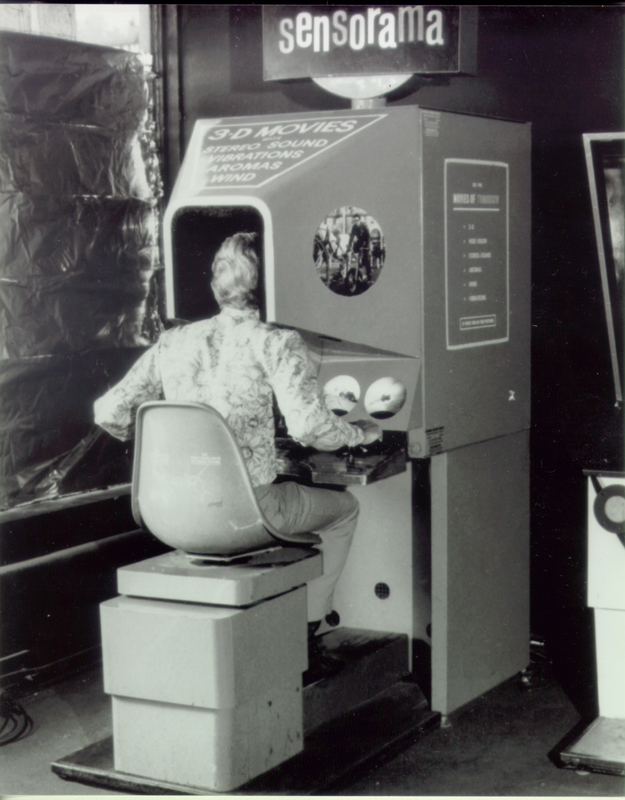
\includegraphics[height=7.5cm]{figures/ch1/sensorama}
  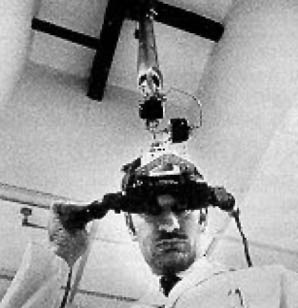
\includegraphics[height=7.5cm]{figures/ch1/ultimateHMD}
  \caption{\label{fig:1_earlyapp}First virtual reality applications: Sensorama Machine (left); The first head mounted display (right).}
\end{figure}

The term ``Virtual reality" in its modern usage was coined and popularized by Jaron Lanier \citep{Lanier1992VR} through his company VPL Research in 1980's. Early definitions of virtual reality are often device-oriented which refer to a certain type of sophisticated computer equipment serving as a medium to connect users to a digitally created space. In the meanwhile, researchers began to discuss and establish conceptual framework of virtual reality, switching from device-oriented definitions to user experience based understanding. Especially, the term ``presnece" or ``telepresence" was introduced to describe the generic perception of being in an artificial environment \citep{Sheridan1992MTV}, which is one of the key notions of VR and will be discussed more thoroughly later on. More elaborated discussions about the history and definition of virtual reality can be found in \citet{Rheingold1991VR}'s book and \citet{Steuer1995Defining}'s paper.

Nowadays, a relatively complete definition of virtual reality was given by another book of \citet{Fuchs2011Book}: ``Virtual reality is a scientific and technical domain that uses computer science and behavioral interfaces to simulate in a virtual world the behavior of 3D entities, which interact in real time with each other and with one or more users in pseudo-natural immersion via sensorimotor channels."

This definition covers three important aspects of virtual reality:

First, virtual reality is both a technical and scientific domain. On one hand, technological progress makes unthinkable experiences become available and provides a hardware platform on which theoretical research of virtual reality is based. For example, CAVE and Head-Mounted Display bring a higher level of visual immersion so that users can actually ``step in" the virtual world and have the sensation of ``being at another place". Real-time tracking devices like leap motion and kinect enable motion capture so that users can interact with computers using natural gestures and other types of body movement. On the other hand, researchers make further investigations of the cause and influencing factors of user's subjective feelings using existing devices, and in return, provide guidelines for the development of future virtual reality systems.

Virtual reality is an extension of human computer interaction (HCI) as we move from traditional desktop to 3D user interface, many of its research methods are inherited or inspired by HCI research work. However, unlike HCI which is design-oriented and tries to find efficient, ergonomic and aesthetic interfaces for interaction, virtual reality aims to ``remove" this interface and let users interact naturally with the virtual world. Virtual reality groups research efforts from various domains as it relies on different technical science domains (e.g. computer science, robotics and automatics etc.) and also on contributions from human and behavioral science (e.g. cognitive psychology, physiology, neurobiology, etc.).

Second, virtual reality possesses two key characteristics which distinguish itself with other existing technologies related to 3D virtual environment: sensorial immersion and real time interaction. In desktop or console based video games, players enjoy real time interaction in the virtual world alone or with other players. They use input devices like joystick, mouse and keyboard which offers very limited sensorial immersion. On the contrary, 3D movies projected on large screens in the cinema give the audience good visual immersion, but no interaction capability. The emergence of virtual reality technology brings great changes to the way we are connected to the virtual world. Having the feeling of being immersed in another world and being able to interact in real time in that world as naturally as in the real world is quite appealing and may change completely the game and movie industries. Of course, the application of virtual reality technology is not limited to these domains, it also has great impact on education, product design, training, etc. Here is a summary of virtual reality applications (ref TODO).

Last and the most important, it reveals three main components of virtual reality system: the virtual environment, the user, and the behavioral interface allowing them to interact. The ``perception, decision and action" loop \citep{Fuchs2011Book} describes how users interact with the surrounding virtual world, which is a transposition of the ``perception, cognition, action" loop demonstrating man's behavior in a real world. As shown in Figure~\ref{fig:1_loop}, the user acts (vocal commands, gestures and other body movements, etc.) on the virtual environment through motor interfaces, and these activities are captured and transferred to the computer system. Then the computer system makes corresponding changes to the virtual environment and generates sensorial reactions (images, sound, haptic, etc.) which are transferred to the user via sensorial interfaces.

\begin{figure}[htb]
  \centering
  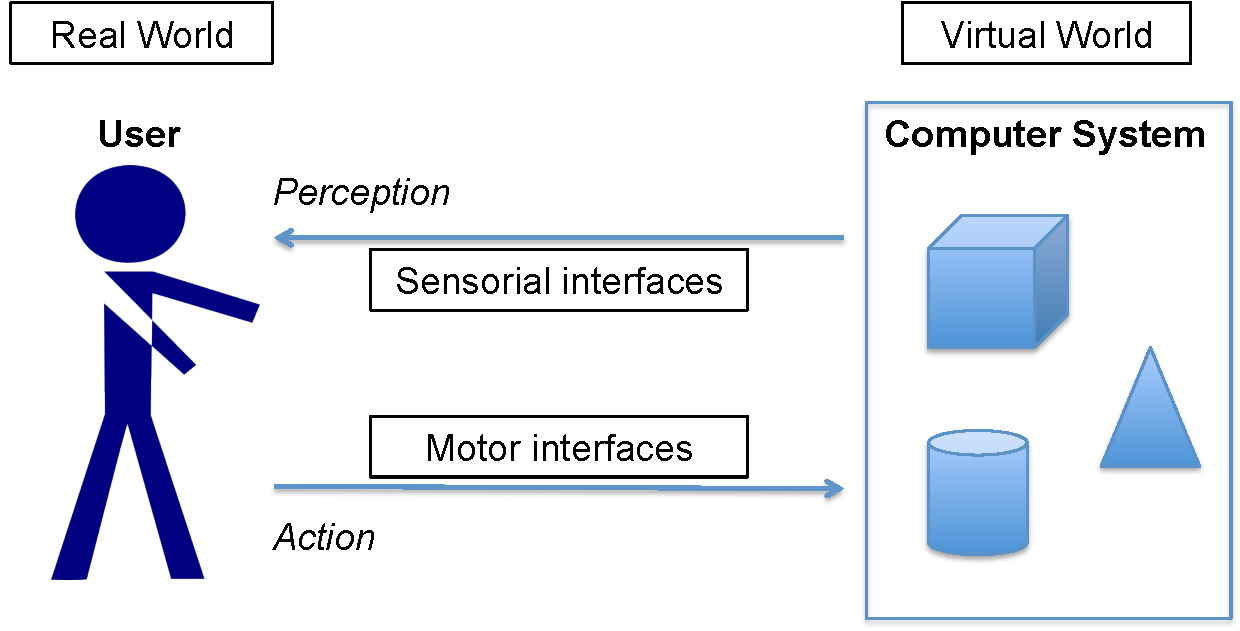
\includegraphics[width=0.9\textwidth]{figures/ch1/loop}
  \caption{\label{fig:1_loop}The ``perception, decision and action" loop in interactive virtual environment.}
\end{figure}

Since the virtual world is totally generated by the computer system, two inherent issues need to be solved: the latency and the sensorimotor discrepancies. The latency is the time lag between the user's action on motor interfaces and the perception of the consequences of this action on the virtual environment through sensorial interfaces. This artifact influences every virtual reality application and may be the source of many problems related to user comfort. The sensorimotor discrepancies is another problem for virtual reality applications. With technical progression, we can simulate more complex phenomenons and provide more interaction through sensorimotor interfaces in the virtual environment, but the real world offers way more information for us to simulate with current technology and the sensorimotor discrepancies will continue to exist.

Now we will discuss in more details about the three components of virtual reality system mentioned above: the virtual environment, the behavioral interfaces and the human inside.

\subsection{Virtual Environment}
Virtual environment is a term often used to describe computer-generated synthetic space, similar to virtual world. However, more strictly speaking, as \citet{Ellis1991VE} explained, an environment is the theater of human activity, so virtual environment is a human-centered notion, not only refers to the digital data that forms an artificial world. For example, according to \citet{Fox2009Guide}: ``A virtual environment is a digital space in which a user's movements are tracked and his or her surroundings rendered, or digitally composed and displayed to the senses, in accordance with those movements." This definition emphasizes that a virtual environment is a virtual space that can react to user's movements and change accordingly.

\citet{Ellis1991VE} summarized three parts which form a virtual environment: content, geometry and dynamics. The content is often organized as scene graph with clear hierarchical structure and inter relationship between objects. Each object possesses a state vector containing properties such as position, orientation, velocity and color, etc. The geometry is a description of an environmental field of action which has dimensionality, metrics and extent, and the dynamics of an environment are the rules of interaction among its contents describing their behavior, such as physical laws (gravity, object collision, etc.). More details on the description of virtual environment can be found in \citet{Ellis1991Pictorial}'s book.

In virtual reality applications, the diversity of origins of the worlds represented in the virtual environment makes virtual reality more than a simple copy of the ``reality" that we live in. As summarized by \citet{Fuchs2011Book}, the virtual world could be a simulation of certain aspects of the real world, but also a completely symbolic or imaginary world. The visual representation of of objects could vary depending on our need, and spatial, temporal and physical laws may or may not be applied in the virtual world. For example, we can visualize and interact with structure of molecules, flow of fluids under different scales \citep{Ferey2009Multisensory, Bryson1996Virtual}, we can also change the speed of light to better visualize and understand phenomenons of relativity \citep{Doat2011NRP}, or the entire world could just be a figment of imagination of an artist or a science-fiction writer.


\subsection{Behavioral Interfaces}
As mentioned in \citet{Fuchs2011Book}'s definition of virtual reality, behavioral interface is a term to describe a type of interfaces that connect the user to the virtual environment. Unlike traditional human computer interfaces which act as a communication tool (e.g. keyboard), behavioral interfaces use the motricity or perceptions of man resulting from his/her behavior in the real world to carry out activities in a virtual world. As shown in Figure~\ref{fig:1_loop}, two types of behavioral interface exist: sensorial interfaces are designed to transfer sensory stimuli from computer to the user while the motor interfaces transfer motor responses from the user to the computer, thus we can also call them sensorimotor interfaces. One of the current challenges of virtual reality is to build more efficient and transparent interfaces based on human sensory channels and motor activities.

\subsubsection{Visual Interface}
As the idiom ``Seeing is believing" states, the visual sense is nearly the most important sensory channel that humans use to discover the real world, which is also true in virtual reality applications. The software and hardware advancements in computer graphics constantly improve the quality of real time three-dimensional images, which allows more complex and photo-realistic rendering. The display used as visual interface should have the following characteristics:

\begin{itemize}
\item Large field of view (FoV) both in horizontal and vertical directions (``borderless");
\item Stereoscopic vision in the entire binocular field of vision;
\item High graphic resolution (pixel density), currently most widely used is 1080p FullHD display, but displays with higher resolution are on the way;
\item Head or eye tracking compatible. Since we can move our head and eyes to look into different directions, it is necessary to assure that user always has perspective-correct view of the virtual scene. This can be achieved by using tracking devices\footnote{see section \ref{sec:tracking}.}
\end{itemize}

A lot of display systems exist nowadays which satisfy all or part of the characteristics listed above, from large immersive rooms and wall displays to table-sized screen, and even portable screens mounted on user's head (see Figure~\ref{fig:1_vi}). They vary in size, form, display technology and aimed applications. Only CAVE (Figure~\ref{fig:1_vi:cave}) and HMD (Figure~\ref{fig:1_vi:hmd}) are designed to provide fully visual immersion. Other displays, on the contrary, can not assure a user to always stay visually inside the virtual world, but they can offer good visual immersion and are better suited for data visualization and 3D object interaction in certain cases. There are also some special display solutions not mentioned above that can provide individual stereoscopic views of 3D models such as the volumetric display \citep{Grossman2008Volum} and holographic display \citep{Lucente1997Holo}, but currently they can only be applied to non-immersive context with even smaller workspace.


\begin{figure}[htb]
  \begin{subfigure}{.3\textwidth}
    \centering
    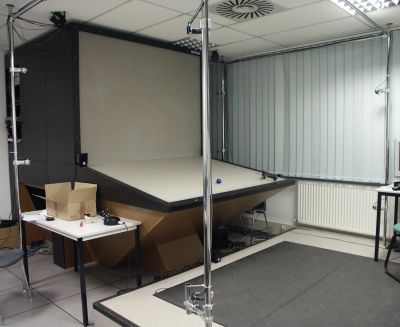
\includegraphics[height=3.5cm]{figures/ch1/workbench}
    \caption{Workbench formed by two separate screens (LIRIS-CNRS).}
    \label{fig:1_vi:bench}
  \end{subfigure}
  \begin{subfigure}{.3\textwidth}
    \centering
    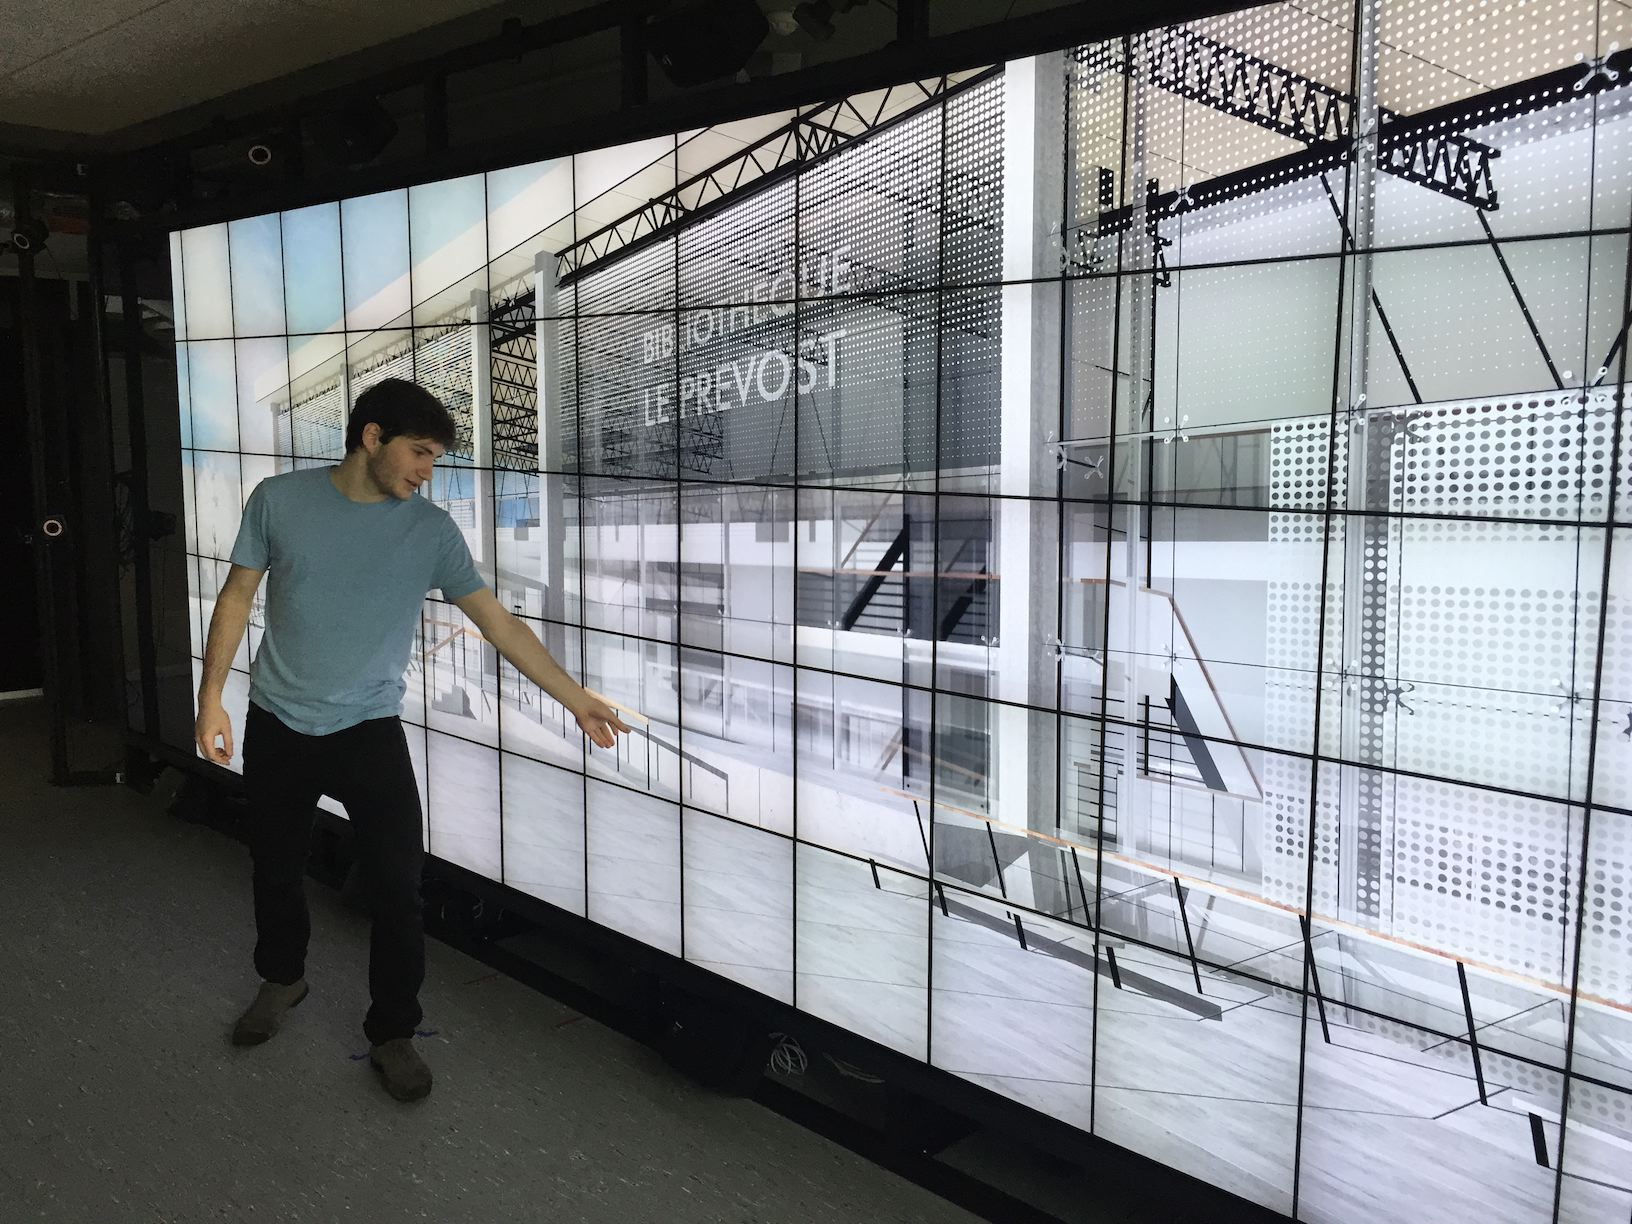
\includegraphics[height=3.3cm]{figures/ch1/wilder}
    \caption{Large image wall composed of high resolution touch screens (WILDER, in$\lvert$situ$\rvert$, LRI).}
    \label{fig:1_vi:wall}
  \end{subfigure}
  \begin{subfigure}{.3\textwidth}
    \centering
    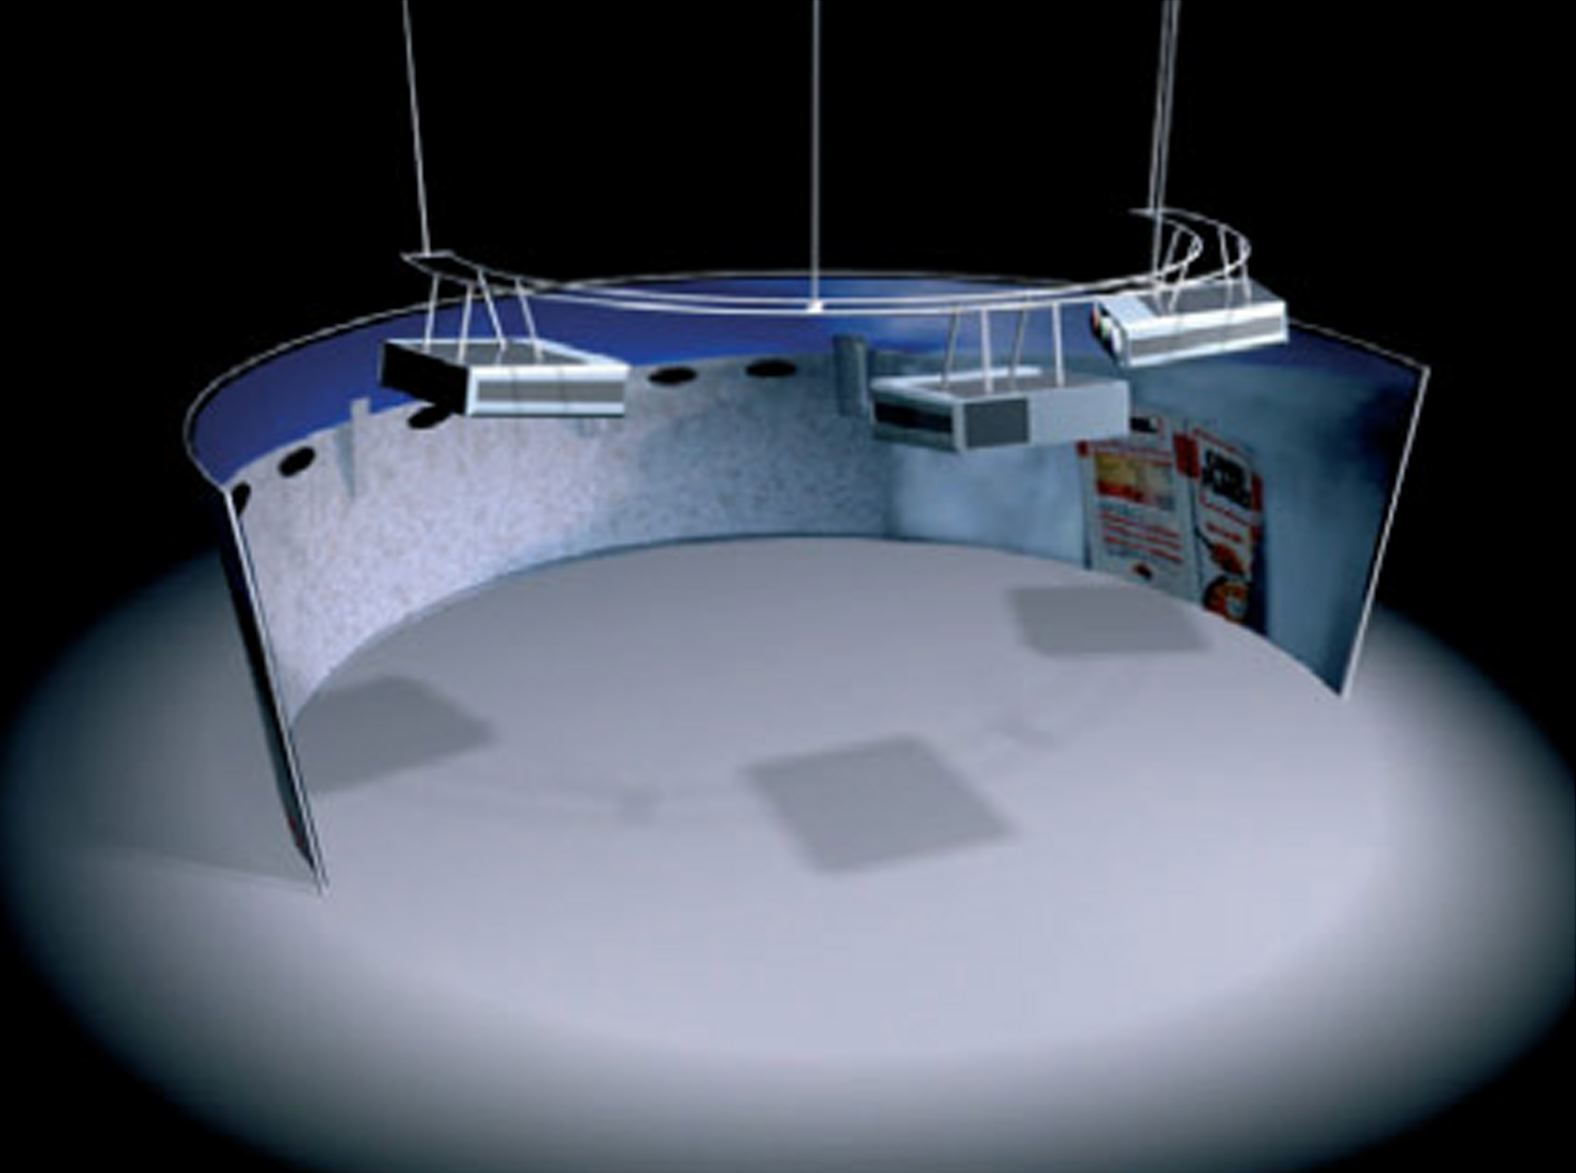
\includegraphics[height=3.5cm]{figures/ch1/icone}
    \caption{The curved panoramic projection screen i-Cone\texttrademark{} \citep{Simon2002Icone}.}
    \label{fig:1_vi:icone}
  \end{subfigure}
  \begin{subfigure}{.5\textwidth}
    \centering
    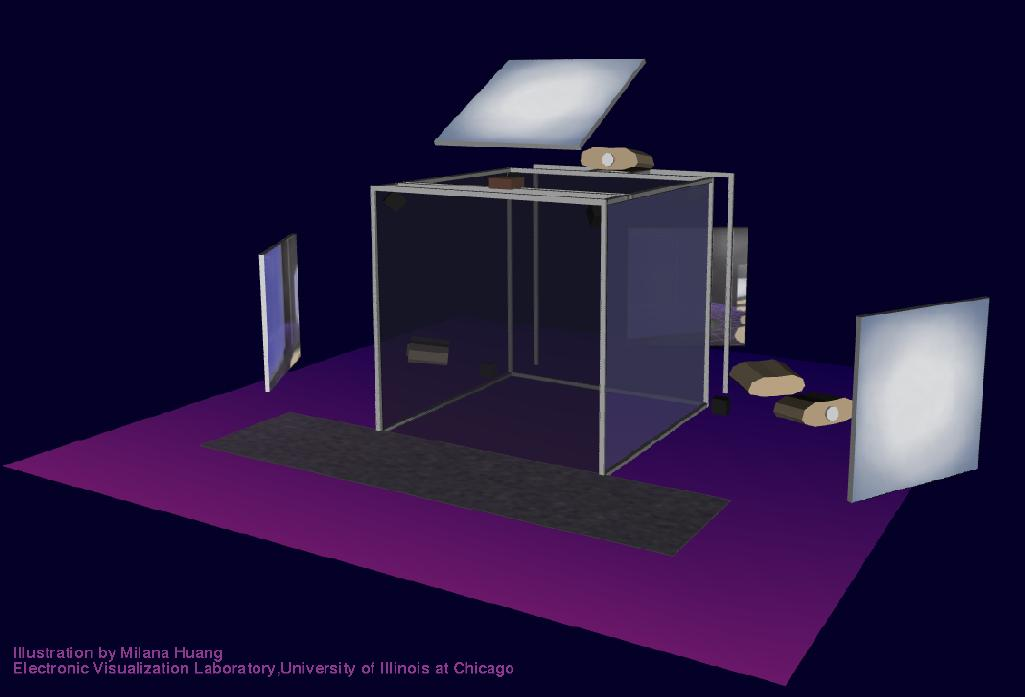
\includegraphics[width=0.9\linewidth]{figures/ch1/cave}
    \caption{CAVE\texttrademark{}: Cave Automatic Virtual Environment \citep{CruzNeira1992CAV}.}
    \label{fig:1_vi:cave}
  \end{subfigure}
  \begin{subfigure}{.45\textwidth}
    \centering
    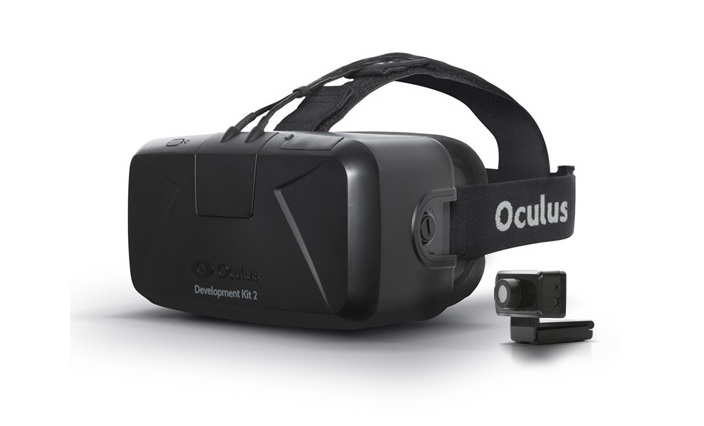
\includegraphics[width=\linewidth]{figures/ch1/oculus}
    \caption{Head-Mounted Display (HMD): Oculus DK2 \copyright{} Oculus VR LLC.}
    \label{fig:1_vi:hmd}
  \end{subfigure}
  
  \caption{\label{fig:1_vi}Different types of visual interfaces.}
\end{figure}


\subsubsection{Audio Interface}
Audio cues are very important for us to perceive events happen in the real world, similarly, the virtual world would be much less appealing if there is no sound. A virtual object would be more ``realistic" if there is a corresponding spatialized sound combined with its visual representation displayed in stereoscopy. For example, a virtual telephone displayed in front of a user with a ringtone coming exactly from that location would make the user believe that the telephone is ringing. A virtual environment filled with ambiance noises and spatialized sound coming from different virtual entities can enhance user's feeling of ``being in that world".

Audio interface has two types of roles: (1) to capture and transfer the sound made by the user (speech, hand clapping, etc.) to the computer system; (2) to transfer audio stimuli from the virtual environment (and from other users connected to the same VE) to the user. The implementation of binaural audio interface managing spatialized sound requires quite complex hardware and software setup which involves lots of research and engineering efforts \citep{Begault1994Sound}. Currently two solutions exist: first, based on Head-Related Transfer Function (HRTF) \citep{Kistler1992HRTF} which is a response that characterizes how an ear receives a sound from a point in space, a binaural sound can be reproduced using a stereo headphone combined with head tracking for one user; second, we can use a group of loudspeakers to reproduce physically the acoustic field based on Wave Field Synthesis \citep{Verheijen1998WFS}, which is independent with listener's position. The first solution is more portable and light-weight while the second is more suitable for large acoustic rooms or theaters.


\subsubsection{Haptic Interface}
The word \textit{haptic} coming from Greek means ``pertaining to the sense of touch". Haptic technology was first developed for tele-operation task so that users can enhance the remote control of machines and devices. Now more and more virtual reality applications integrate haptic interface so users can ``tele-operate" objects in the virtual world. With the help of haptic feedback, users can not only perceive virtual objects' different properties (shape and texture, etc.) by touch, but also interact physically with them (e.g. to push a virtual forklift \citep{Martin2012Forklift}). Being able to imply the sense of touch in the interaction within virtual environment is a huge step forward in aim of creating fully immersive experience in the virtual world, though lots of technical issues remain to be solved. 

Generally speaking, haptic technology aims to recreate the sense of touch by applying two kinds of stimuli to the user: tactile feedback and proprioception feedback. Tactile sensation is formed from several modalities including pressure, skin stretch, vibration and temperature, while proprioception feedback concerns the feeling of having physical contact between different parts of human body and the virtual environment. Many haptic devices on the market provide force feedback and vibration for part of the human body, especially the hands and arms, for example, electromechanical haptic arms shown from Figure~\ref{fig:1_hi:phantom} to \ref{fig:1_hi:scale1} have different workspace size and accessible force range to provide from desktop-based to room-sized haptic interaction. Some glove-shaped (Figure~\ref{fig:1_hi:dexmo}) or string-based (Figure~\ref{fig:1_hi:spidar}) devices equipped with finger-level motors can support even finer force feedback to the user for actions like object grasping and manipulating with fingers. However, there seems still no easy solution to provide full-body haptic feedback and tactile experience with relatively complex objects, so sometimes real objects (called props or tangible interfaces) are introduced into the virtual environment for passive haptic feedback in specific applications (Figure~\ref{fig:1_hi:prop}).

\begin{figure}[htb]
  \begin{subfigure}{.3\textwidth}
    \centering
    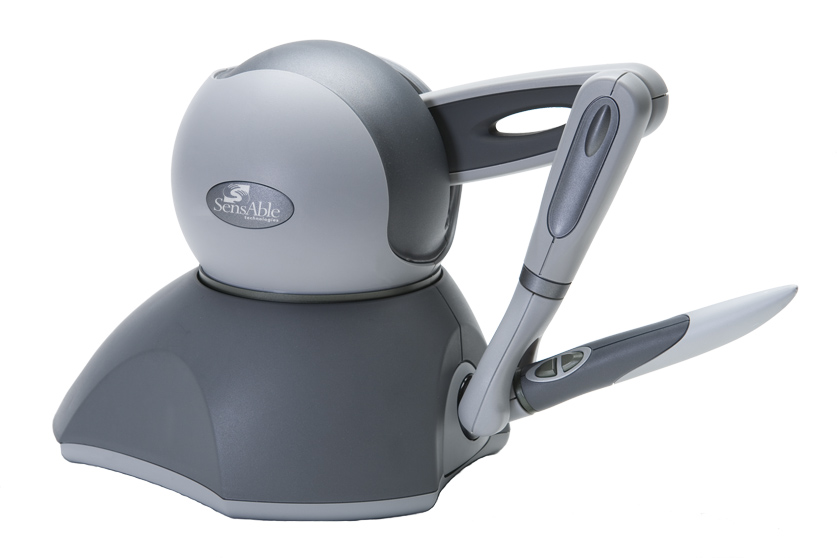
\includegraphics[width=0.8\linewidth]{figures/ch1/phantom}
    \caption{PHANTOM\textregistered{} Omni haptic arm \copyright{} Sensable.}
    \label{fig:1_hi:phantom}
  \end{subfigure}
  \begin{subfigure}{.3\textwidth}
    \centering
    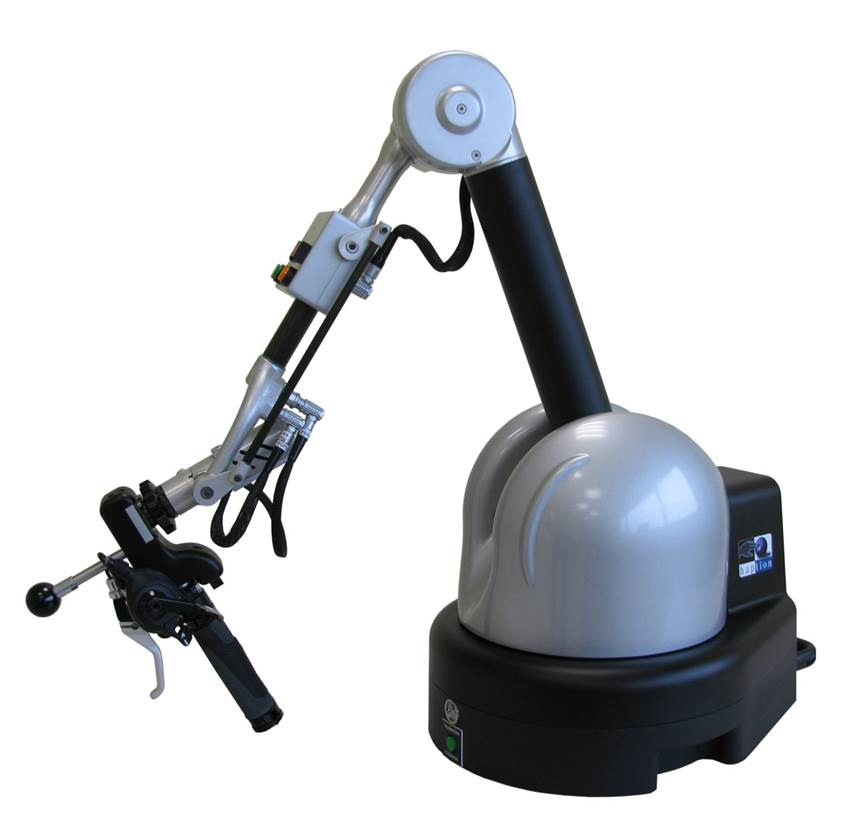
\includegraphics[width=0.8\linewidth]{figures/ch1/virtuose}
    \caption{The Virtuose 6D haptic arm \copyright{} Haption.}
    \label{fig:1_hi:virtuose}
  \end{subfigure}
  \begin{subfigure}{.35\textwidth}
    \centering
    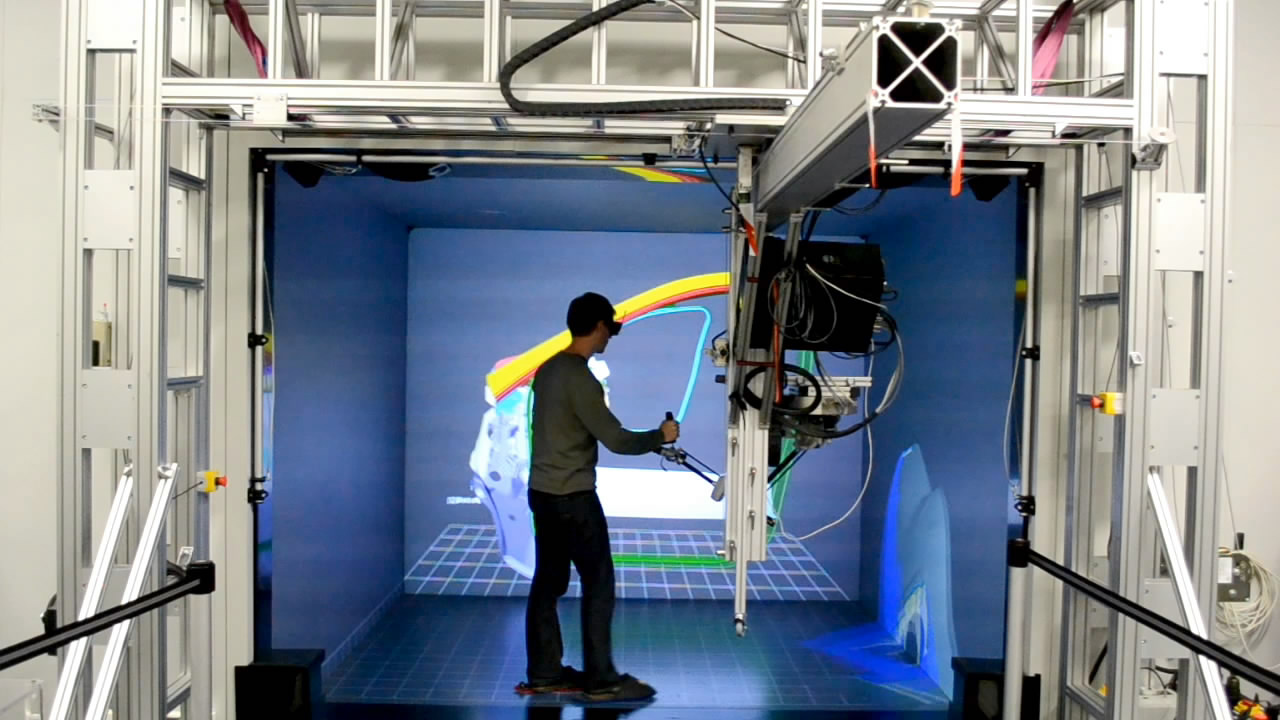
\includegraphics[width=0.9\linewidth]{figures/ch1/scale1}
    \caption{Scale one room-sized haptic solution \copyright{} Haption.}
    \label{fig:1_hi:scale1}
  \end{subfigure}
  \begin{subfigure}{.3\textwidth}
    \centering
    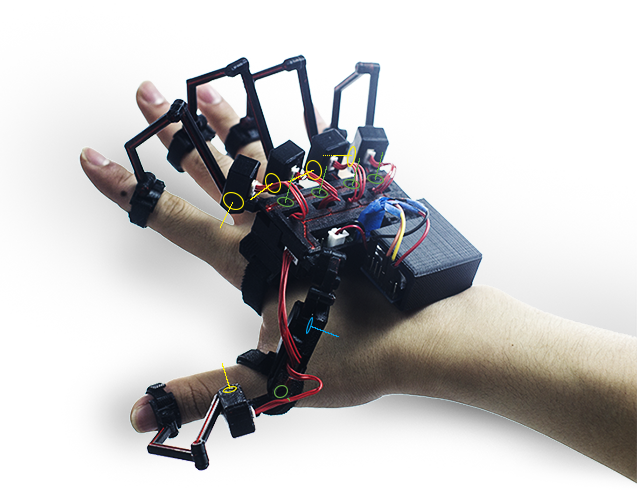
\includegraphics[width=\linewidth]{figures/ch1/dexmo}
    \caption{Dexmo\textregistered{} wearable mechanical exoskeleton \copyright{} Dexta Robotics.}
    \label{fig:1_hi:dexmo}
  \end{subfigure} 
  \begin{subfigure}{.35\textwidth}
    \centering
    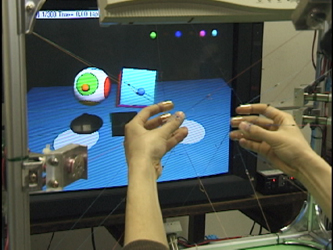
\includegraphics[width=0.9\linewidth]{figures/ch1/spidar}
    \caption{SPIDAR: string-based force feedback device \citep{Sato2002SPIDAR}.}
    \label{fig:1_hi:spidar}
  \end{subfigure}
  \begin{subfigure}{.32\textwidth}
    \centering
    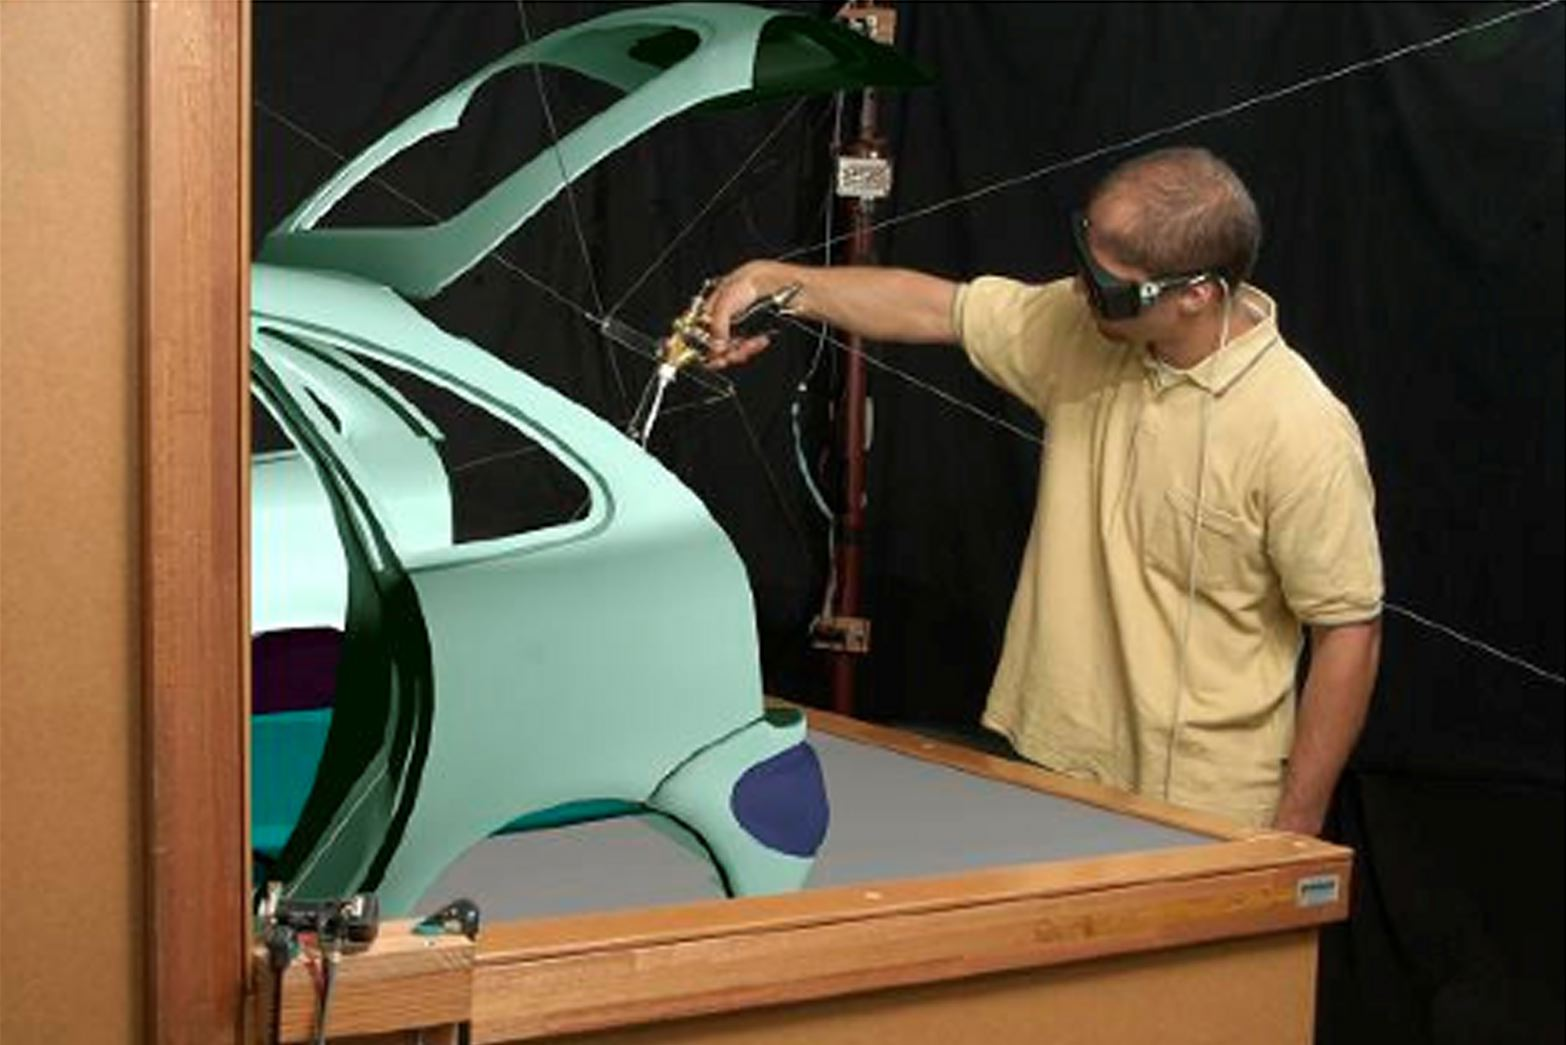
\includegraphics[width=0.9\linewidth]{figures/ch1/prop}
    \caption{The putty gun served as prop offering passive haptic feedback \citep{Ortega2005Prop}.}
    \label{fig:1_hi:prop}
  \end{subfigure}
  \caption{\label{fig:1_hi}Different types of haptic interfaces.}
\end{figure}

\subsubsection{Tracking Interface}
\label{sec:tracking}
The goal of tracking interface is to capture and transfer user's motor information as input for the computer system to update the virtual world and to generate proper sensorial stimuli (visual, audio, etc.) for the user. Tracking an entity in 3D space requires six degrees of freedom (DoF) information: three for position in form of a vector $(x, y, z)$ and three for orientation in form of Euler angle $(\theta{x},\theta{y},\theta{z})$.

In many virtual reality applications, it is sufficient to track user's head and dominant hand to respectively ensure correct visual rendering according to user's viewpoint and to allow basic interaction (e.g. object selection) in the virtual world. However, full-body movement tracking (motion capture) is increasingly demanded to enrich interaction scenarios and to enhance the level of immersion. Moreover, when multiple users are inside the same virtual environment, full-body tracking combined with decent avatar representations largely facilitate social human communication (which will be further discussed in section~\ref{sec:user-com}) by transferring subtle non-verbal cues (postures and gestures) among users. Recently, eye tracking technology has received a lot of attentions for its potential benefits in many domains \citep{Duchowski2007Eye} and it will become an important part of tracking interface for virtual reality systems.

Tracking interface can be implemented with different physical principals, including mechanical, electromagnetic, optical or acoustic methods \citep{Meyer1992Survey}. Although no single technology works for all purposes, certain methods work quite well for specific applications \citep{Welch2002Survey}. The new trend now is to combine different tracking technologies into one product to get better tracking quality, e.g. the hybrid suit from ART\footnote{http://www.ar-tracking.com/products/motion-capture/hybrid-suit} is a combination of optical, mechanical and magnetic trackers. Video based tracking devices using computer vision methods, such as kinect and leap motion (Figure~\ref{fig:1_video_tracking}), are also getting more popular because of their low cost and easy setup procedure.

\begin{figure}[htb]
  \begin{subfigure}{.5\textwidth}
    \centering
    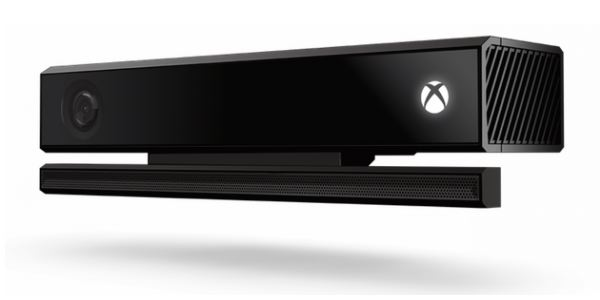
\includegraphics[height=3cm]{figures/ch1/kinect}
    \caption{The Kinect (version 2) \copyright{} Microsoft.}
    \label{fig:1_video_tracking:kinect}
  \end{subfigure}
  \begin{subfigure}{.5\textwidth}
    \centering
    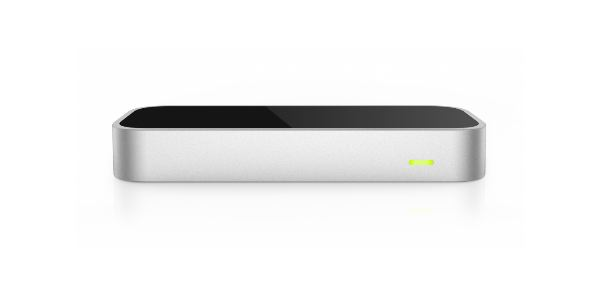
\includegraphics[height=3cm]{figures/ch1/leap}
    \caption{Leap motion controller \copyright{} Leap Motion.}
    \label{fig:1_video_tracking:leap}
  \end{subfigure}
  \caption{\label{fig:1_video_tracking}Video-based tracking interfaces.}
\end{figure}

\subsubsection{Other Interfaces}
Apart from major sensory channels like vision, audio and the sense of touch, the human sensorimotor system is way more complex and all senses could contribute to the feeling of presence in the virtual world. For example, \citet{Matsukura2011MSF} designed a multi-sensorial field (MSF) display which can generate air flow and odor vapors to simulate odor distribution in the virtual world, and \citet{Narumi2011Flavors} developed a ``Pseudo-gustation" method to change the perceived taste of food by changing its appearance and scent. However, integrating all types of behavioral interfaces into a single virtual environment remains a challenge because of the complexity and compatibility issues of different hardware and software solutions. 


\subsection{Human in Virtual Environment}
As we discussed before, virtual reality is a human-centered research domain. Technical advancement concerning the modeling of virtual world and the design of behavioral interfaces all serve to provide a better feeling of ``being in another world" (presence) for the human in virtual environment. So to understand human activity and sensation at perceptual and cognitive levels is a key to the success of virtual reality system.

\subsubsection{3D Interaction}
\label{sec:3D_inter}
The interaction between the user and 3D virtual world begins once he/she is inside the virtual environment, and these human activities can be divided into some basic behaviors named Virtual Behavioral Primitives (VBP) \citet{Fuchs2011Book}. VBPs can be grouped into five categories:

\begin{itemize}
  \item observation;
  \item moving;
  \item acting;
  \item communicating with others;
  \item application control.
\end{itemize}

In the list above, except for application control, these activities are very similar to what people practice in the real world. Observation is our first triggered action after we dived into a virtual environment, which is a relatively passive action. The only interaction part is that when user turns head or has ocular movements (captured with eye tracking), the system will adapt the visual and audio rendering accordingly. Moving or navigation in the virtual world is also a basic interaction for the user to accomplish various tasks like object searching or transporting, way finding, sightseeing, etc. Besides natural walking, many virtual navigation metaphors are developed to effectuate more efficient virtual viewpoint control under different specific conditions (more details to be presented in Chapter \ref{chapter:nav_cohab}). Regarding ``acting", which is a vague notion, is further broke into object selection, manipulation and symbolic input by \citet{Bowman2004UIT}. The way we interact with virtual object is still quite different than with real objects due to technical limitations (e.g. lack of detailed and robust haptic feedback), thus many interaction metaphors are proposed to enable other forms of interaction \citep{Hand1997Survey}.


\subsubsection{Presence}
Sensorial immersion offered by immersive virtual environment can give user the illusion of ``being there" or the feeling of presence \citep{Heeter1992Presence}, which is a central concept of virtual reality. Presence, or telepresence, is used to describe user's subjective feeling of being immersed in a virtual environment, while the term ``immersion" is a product of technology that facilitates the production of multimodal sensory stimuli to the user \citep{Slater1994DepthPre, Bystrom1999Model}. Presence in virtual reality is a psychological state relying on sensorimotor illusion, which is different than the presence feeling at cognitive level that we have in dreams or by reading a book.

This general definition of presence is shared by many researchers, but there are still nuances in the explanations and interpretations of the definition.

\citet{Slater1994DepthPre} suggest that presence is assessed by the subjects as their sense of ``being there", the extent to which they experienced the virtual environments as more the presenting reality than the real world in which the experiment was taking place, and the extent to which the subject experienced the virtual environments as places visited rather than images seen. Then \citet{Kim1997Telepresence} describe presence as the product of two factors: (1) ``the arrival" or the feeling of being ``there" in the virtual environment, and (2) ``the departure" or the feeling of not being there ``there" in the physical environment. ``The arrival" (or one's involvement in a virtual environment) occurs when an individual concentrates their energy and their attention onto a stimulus and the events happening in the virtual environment, thus permitting the augmentation of the degree of involvement or of presence. Similarly, \citet{Witmer1998MPV} relate presence in part to the concept of attention: presence may vary across a range of values that depends in part on the allocation of attentional resources. They think that both involvement and immersion are necessary for experiencing presence. \citet{Lombard1997Heart} have attempted to offer another explanation of the concept of presence as they define presence as the perceptual illusion of non-mediation, which focuses on the transparency of behavioral interfaces.

Studies have shown that the level of presence has not only a pronounced effect on user's task performance \citep{Dangelo2008Benefits}, but also an impact on the social relationship between collaborators \citep{Slater2000Small}. To step further towards a more complete virtual reality system which could invoke higher level of presence for the user, it is important to identify factors that contribute to the formation of presence and to establish related evaluation models. Being an ongoing research topic, existing models for presence measurement are restricted to subjective rating through questionnaires \citep{Usoh2000Using, Witmer1998MPV}. The use of physiological measures for presence evaluation has been attempted \citep{Meehan2002Physiological}, but we still need more follow-up studies to design a complete evaluation model based on physiological indicators. A detailed analysis of influencing factors of presence and a taxonomy for presence measurement methods are presented by \citet{Schuemie2001Pres}.


\subsubsection{Cybersickness}
Cybersickness is a polygenic \citep{Kennedy1992Simulator} and troublesome problem with current virtual reality technology. Cybersickness, or simulator sickness (they may be different according to \citet{Stanney1997Cybersickness}), is the tendency for some users to exhibit symptoms that parallel symptoms of classical motion sickness both during and after being immersed in virtual environments. Short-term symptoms of cybersickness have been identified after repeated studies \citep{Lawson2002Signs}, but currently we still know little about its long-term effects. It is essential to understand the causes for cybersickness and to find ways to eliminate it for better use of virtual reality technology.

Researchers have tried to identify factors that are susceptible to cause cybersickness when using a virtual environment. For example, \citet{Rich1996AICS} examined the relationship between sensory compatibility and cybersickness symptoms, while \citet{So2002Scene} emphasized that the visual complexity of the virtual scene should also be taken into consideration. Technical issues such as lags \citep{Pausch1992Literature}, flickers \citep{Harwood1987Temporal}, and individual factors like gender \citep{Biocca1992Will} and age \citep{Reason1975Motion}, all have some influences on the severity of cybersickness symptoms. A more complete list of primary factors that contribute to the cause of cybersickness was provided by \citet{LaViola2000DCV}. He also gave an interesting discussion on three conflicting theories that try to explain the occurrence of cybersickness.

Currently, to evaluate the severity of cybersickness, the Simulator Sickness Questionnaire (SSQ) \citep{Kennedy1993SSQ} remains the reference tool. SSQ groups all symptoms around three main factors: nausea (nausea, stomach awareness, etc.), oculomotor (eyestrain, blurred vision, etc.) and disorientation (dizziness, vertigo). The development of various physiological measurements also begins to show interesting correlation between cybersickness symptoms and various physiological indicators \citep{Kim2005Characteristic, Min2004Psycho, Sugita2008Quantitative}. However, further research efforts are required to establish a valid cybersickness evaluation model based on physiological indicators. The study of physiological responses of human body when exposed to virtual environment will also help us to better understand the cause of cybersickness.

\subsubsection{Workspace Management}
When interacting in an immersive virtual environment, user's sensory channels are partly blocked by the computer system. However, this does not change the fact that the user is still in the real world, thus he/she is constrained by limits of the physical workspace, for example, the user can not cross real walls or screen displays. The implication of these real world constrains on the use of immersive virtual environment is a major issue of this manuscript and will be discussed in Chapter \ref{chapter:nav_cohab}).


\subsection{Summary}
This first part of Chapter \ref{chapter:context} gives a brief introduction of virtual reality around its three main components: virtual environment, behavioral interface and the user. Key notions like presence and cybersickness, as well as different hardware implementations of virtual reality system are presented, so they can be used directly later on in this manuscript. 

% -------------------------------------------------------------------------------------------------
\newpage

\section{Computer Supported Collaboration}
The development of communicational technology changes the way people work together, for example, telephone and telegraph make the exchange of information much faster than paper-based media. Later on, with the boom of the Internet, emails, forums, video conferences create a tighter link among remote collaborators. However, networked collaboration still faces a lot of difficulties in terms of communication and coordination. For example, how a group of coders can contribute to the same project remains a non-trivial job despite using versioning tools like svn or git.

In 1984, Irene Greif of MIT and Paul M. Cashman of Digital Equipment Corporation organized a workshop attended by people from various domains interested in using technology to support people in their work. In this workshop the term Computer Supported Cooperative Work (CSCW) was first mentioned \citep{Grudin1994Computer}, then it becomes a research domain attracting world-wide interests. CSCW studies how computer systems could enable a group of people connected by network to work together efficiently, or as stated by \citet{Carstensen1999CSCW}: ``how collaborative activities and their coordination can be supported by means of computer systems". More details about the history, state of the art and research issues of CSCW can be found in the book by \citet{Beaudouin1999CSCW}.


\subsection{Characteristics of Collaborative Work}
We can learn many things from observation of people working and collaborating in the real world to get some insights into the nature of collaborative work \citep{Churchill1998CVE}. Here are some general points to summarize characteristics of collaborative work:

\paragraph{Collaboration is human-centered} The number and profile of people involved in the task define the general organization for collaboration. For example, small groups are likely to work together in real time with more flexible schedules, communicate informally and share information with minimal cost, while large groups need much more efforts for coordination and more adapted communication technology. The profile of collaborators also matters, if one person is way more experienced than others, it is better to have a leader-follower mode so everyone works around this leader. However, if working capacity is homogeneously distributed and especially, each one has his/her own expertise, it is better to work with equal responsibility for the task.

\paragraph{Collaboration is task-oriented} The nature of the task defines the spatial and temporal constrains for collaboration, or we can say that sometimes people need to collaborate because of some spatial or temporal issues and the task can not be done without combining efforts from different actors. For example, tasks like painting a wall or repairing a car together require people to be co-located, other tasks like operating a TV live show, or having a video conference need synchronous actions. Moreover, complex tasks often consist of different components with inherent logical links and the task can only be accomplished with a certain procedure.  

\paragraph{Awareness is the base of coordination} Awareness is one's knowledge of task related activities, especially activities of others. As stated by \citet{Dourish1992Awareness}, awareness is an ``understanding of the activities of others, which provides a context for your own activity". This ``context" allows an individual to evaluate his/her actions with respect to group goals and work progress. In addition, awareness may also refer to the knowledge of the state of a task related object (e.g. the history and current state of the shared document for group editing task) and the working atmosphere (whether there is an emergency, whether people are under pressure, etc.).


\paragraph{A shared context is essential} A shared context allows group members to ``stay on the same page" (shared understanding), which largely facilitates their communication and coordination. We can call it a \textit{common ground} \citep{Clark1991Grounding} or \textit{team situation awareness} \citep{Salas1995SA} which is based on the situation awareness of each individual. In conventional situations, a shared context is naturally established by a shared physical and social space. For example, two workers are in the same room, there will not be confusion when one points to a table and says ``Let's move it to the corner". When people are distributed and connected by computer network, it is essential for a successful collaborative system to maintain a shared context by sharing artifacts and activities.

\paragraph{Multiple viewpoints are helpful} A complex task should have multiple representations, each offering a different point of view of the problem or focusing on a specific subtask. In certain cases, one individual may require multiple representations to reflect different aspects of their task, whilst in other cases people with different profiles and skills may require tailored representations to provide information specific to their tasks. Taking an example from \citet{Churchill1998CVE}, people taking part in the architectural design review of a building might only want to see features relating to their specialty in detail. So an electrician might only want to see detailed wiring plans, but not necessarily the plans for the plumbing, except in cases where there was a potential conflict. There are more reasons to vary the representation of a task in a broader social context, for example, companies involved in a same project often need to keep their sensitive data or workflow from others. So when designing computer supported collaborative system, ``WYSIWIS" (What You See Is What I See) \citep{Stefik1987WYSIWIS} may not be a proper choice in many cases.

\paragraph{Transition between shared and individual activities is required} Collaborative scenarios usually contain different coupling stages \citep{Gutwin1998Design, Lissermann2014PMC}: \textit{closely-coupled stage} to solve problems in group and \textit{loosely-coupled stage} to tackle individual subtask. So collaborative work involves the interleaving of individual and group effort, which requires explicit communication and coordination between collaborators. For example, in a car assembly task, workers may need to go to storehouses and fetch a certain component for change from time to time, and then come back to the assembly work. This task contains both individual object-searching and closely coupled interactions for the assembly work. \citet{Isenberg2012Co} further identified a series of eight different collaboration styles and activities that participants adopted during a working session around an interactive table. So a collaborative system should manage group workspace as well as personal workspace and allow active transition between shared and individual activities.


These characteristics help us to understand the process of collaborative work and offer a guideline for the design of computer supported collaborative system. \citet{Okada2007Collab} proposed a multi-layered hierarchical framework which shows a clear picture of different elements contributing to the collaboration and a structural link between aforementioned characteristics. As shown by Figure~\ref{fig:1_collab_model}, the model consists of four layers and each layer is based on the layer below: spatial and temporal coexistence enables awareness of others' activities, which then allows the exchange of views and opinions, the sharing of knowledge and information, and the distribution of work and operations. At the highest level, the sharing of activities enable the final collaboration between multiple actors with the balance between assertions and cooperations (negotiation).

\begin{figure}[htb]
  \centering
  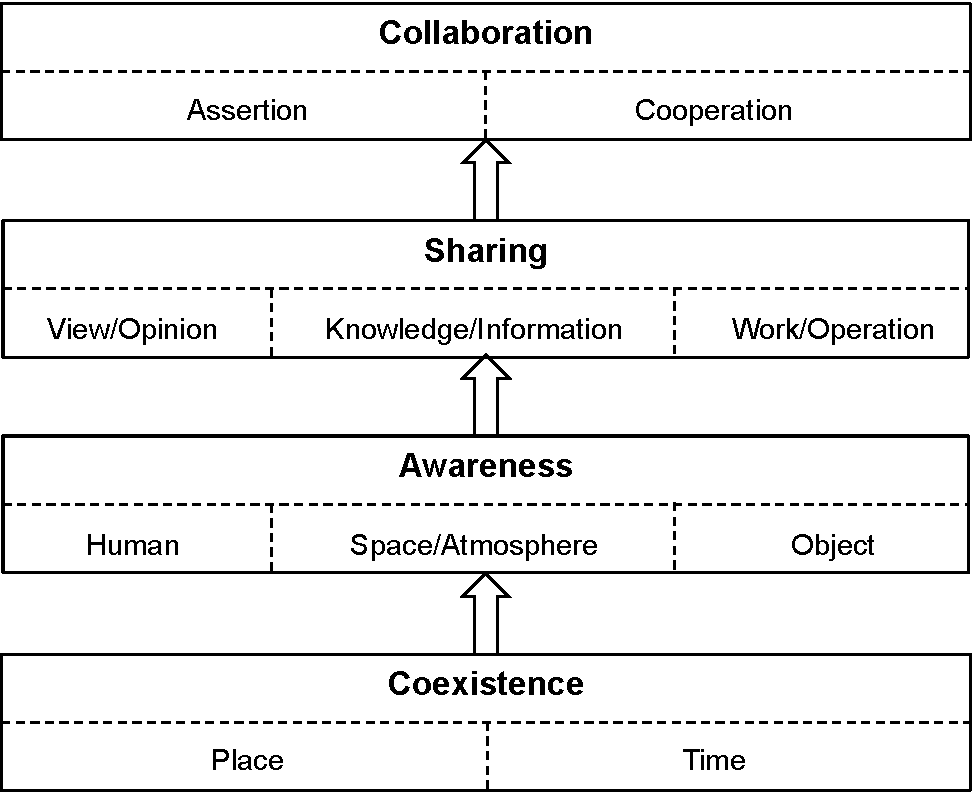
\includegraphics[width=0.6\textwidth]{figures/ch1/collab_model}
  \caption{\label{fig:1_collab_model}A hierarchical collaboration model from \citet{Okada2007Collab}.}
\end{figure}

\subsection{Groupware}
Being the central interest of CSCW, groupware is a type of computer-based systems designed to support a group of people to work together. \citet{Ellis1991Groupware} defined groupware as the following: ``computer-based systems that support groups of people engaged in a common task (or goal) and that provide an interface to a shared environment".

Groupware implementations can be grouped by a conceptual time-space matrix \citep{Johansen1988Groupware, Ellis1991Groupware} regardless of involved technology. As shown in Figure~\ref{fig:1_tsmatrix}, this matrix has a temporal dimension (whether users work the same time or asynchronously) and a spatial dimension (whether users are co-located or geographically distributed).

\begin{figure}[htb]
  \centering
  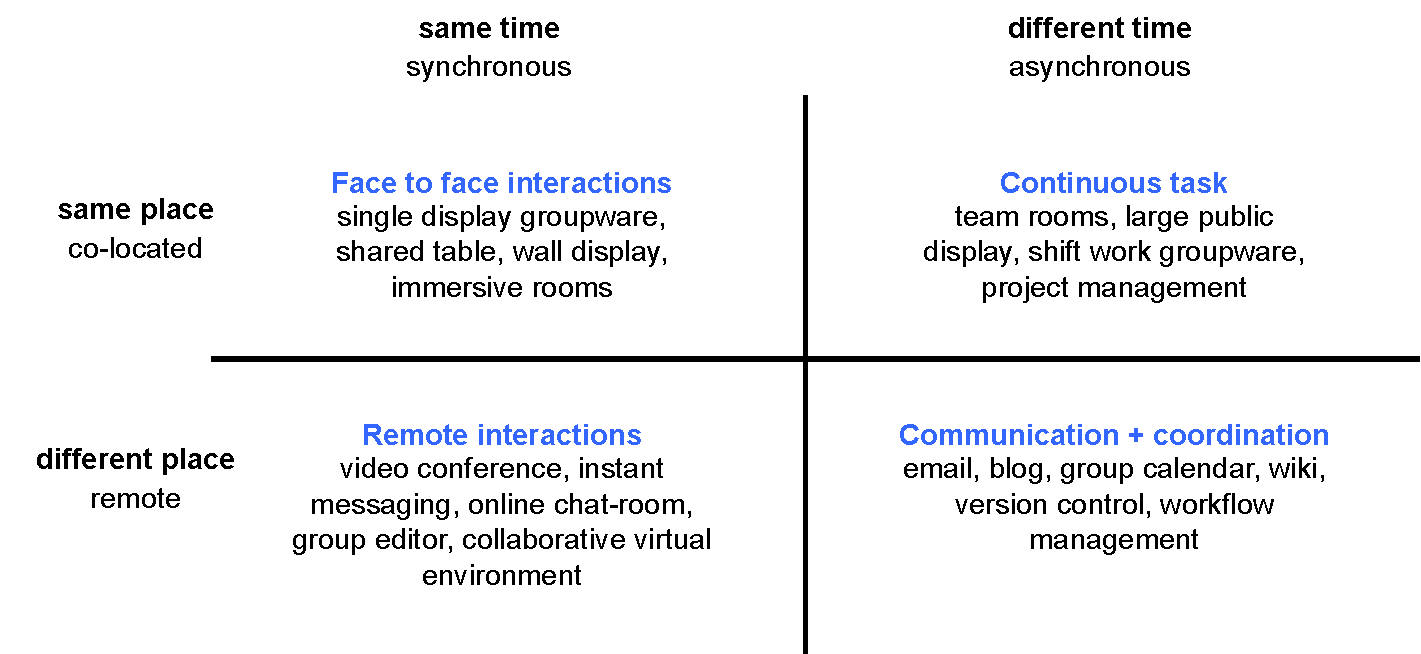
\includegraphics[width=\textwidth]{figures/ch1/tsmatrix}
  \caption{\label{fig:1_tsmatrix}The time-space matrix for groupware classification.}
\end{figure}

This typology of groupware based on time-space matrix is not aimed to provide strict rules to put every groupware application into one of the categories. Sometimes both synchronous and asynchronous communications are supported by a given device (e.g. two groups of users work on a wall display with results left by a previous group), and the used technology does not imply geographic distance between users (e.g. forwarding an email to a co-worker in the same room). However, it shows an overview of existing CSCW systems depending on the context of a system's use. It also offers a guideline for groupware design concerning temporal and spatial constrains. For example, synchronous applications need management of concurrent resource access and live communication between users, and groupware connecting remote users need to carefully choose the network architecture (server-client, peer-to-peer, etc.) to be used and to take into consideration the network latency.

Another taxonomy by \citep{Grudin2012Taxonomy} divides collaborative activities into three functional categories: communication, information sharing and coordination. The accomplishment of a collaborative task often requires all three types of activities. For example, when several authors of a book use a group editor to finish their work together, they need to have a shared version of the document and a clear assignment of different unfinished parts to corresponding authors, and also real-time communications by means of instant messages or audio meetings and asynchronous communications by leaving comments and annotations.


\subsection{Collaborative Virtual Environment}
\subsubsection{Definition}
A Collaborative Virtual Environment (CVE) refers to a virtual environment that enables multiple users to interact and to achieve collaborative tasks. CVEs provide a potentially infinite, graphically realized digital landscape within which multiple users can interact with each other and with simple or complex data representations \citep{Churchill1998CVE}. 

CVE differs from traditional groupware applications (e.g. email, instant messages, video conference, etc.) in that, instead of connecting people from different locations, CVEs create a virtual world and ``put" users and task related information directly in that world. This virtual world naturally provides users with a common spatial and social context for collaboration. CVEs are also different from other content sharing groupware such as group editors and group calendars because CVEs are multi-function and multi-purpose platforms that can support many forms of communication both for routinized and highly flexible tasks. Users have more degrees of control over the communication with others (free to navigate and encounter people) and more types of interactions with digital objects inside a malleable virtual space.

A lot of CVE applications exist from early prototypes (e.g. DIVE \citep{Carlsson1993DIVE}, NPSNET \citep{Macedonia1994NPSNET} etc.) appeared during 1990's (Figure~\ref{fig:1_cve:dive}), to more developed systems like MASSIVE-3 \citep{Greenhalgh2000MASSIVE} and ANTS \citep{Lopez2003ANTS}, etc. The general framework of CVE is gradually stabilized and standardized since then. Now mature CVE systems are widely applied and become the major trend in the game industry, there are enormous commercial products like online communities (e.g. Active Worlds\footnote{https://www.activeworlds.com}) (Figure~\ref{fig:1_cve:aw}) and collaborative games like MMORPGs\footnote{Massively Multiplayer Online Role-Playing Games} which attract millions of users \citep{Brown2004CSCW}. More information about the history and current status of CVEs are presented by \citet{Joslin2004CVE}.

\begin{figure}[htb]
  \begin{subfigure}{.5\textwidth}
    \centering
    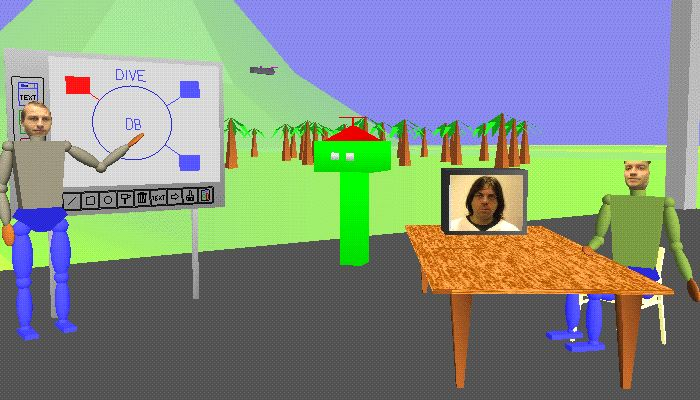
\includegraphics[width=\linewidth]{figures/ch1/dive}
    \caption{A virtual meeting within the DIVE platform.}
    \label{fig:1_cve:dive}
  \end{subfigure}
  \begin{subfigure}{.5\textwidth}
    \centering
    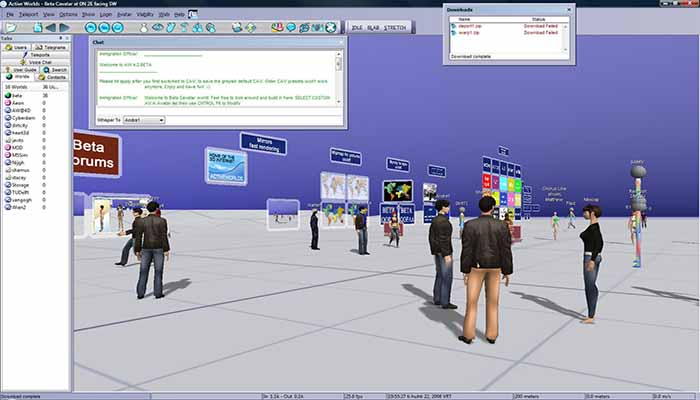
\includegraphics[width=\linewidth]{figures/ch1/activeworld}
    \caption{The Cavatar world from Active Worlds.}
    \label{fig:1_cve:aw}
  \end{subfigure}
  \caption{\label{fig:1_cve} Some examples of existing CVE applications.}
\end{figure}


\subsubsection{Issues and Challenges}
\label{sec:cve-issue}
The emergence of CVEs comes along with technical issues due to the complexity of such system. Supporting rich social interaction in densely populated virtual worlds requires addressing a variety of technical challenges. Here is a list of technical issues that need to be addressed inspired by the work of \citet{Benford2001CVE} and \citet{Joslin2004CVE}:

\begin{itemize}
\item Scene management: how to merge events and keep data consistency among different sites, how to segment a virtual world into smaller sections \citep{Kazman1993Making};
\item Network topology: choose among server-client, peer-to-peer or hybrid structure to reduce traffic loads and improve data distribution efficiency;
\item Compression: how to compress the data to be transmitted knowing that real time interaction between multiple users can generate huge amount of data, especially with sophisticated virtual human \citep{Capin1998Efficient};
\item Personal viewpoint: design software model to support ``subjective" view on the shared world \citep{Smith1996CVE};
\item Human computer interface: using virtual reality technology to convey more information for natural interaction and social communication;
\item etc.
\end{itemize}

Human factors are also crucial to the design and effective use of CVEs as a new type of social community. Here we group research questions around four topics: 

\begin{itemize}
\item Social conventions: are the social conventions in the real world still applicable in the shared virtual world \citep{Becker1998Social}? What has or has not changed?
\item User embodiment: how the virtual representations (simple object, robot, humanoid avatar, etc.) influence their communication? How to design the body image of a user to provide information such as identity, activity, availability, mood and many other factors \citep{Benford1995Embodiment}? 
\item Awareness: how to be aware of other people's intention and perceptual capabilities (e.g. size of field of view) in the virtual world \citep{Benford1994Awareness}?
\item Social communication: how social communications are supported in CVEs compared to cases in real world \citep{Bailenson2006Long}?
\end{itemize}

\citet{Otto2006Review} also give a summary of factors that influence collaboration in CVEs by grouping them into different levels.

\subsection{Summary}
This second part of Chapter \ref{chapter:context} summarizes characteristics of collaborative work in the real world and their implications for the design of computer supported collaboration systems (groupware). CVE as a flexible and multi-function platform attracts research interests from both CSCW and virtual reality communities. Although there are still many technical and human-related issues to be solved, CVEs already show great potential for supporting efficient and seamless collaboration in a rich social context.


% -------------------------------------------------------------------------------------------------
\newpage

\section{Immersive Collaborative Virtual Environment}
As stated in the previous section, CVE is developing as a convergence of research interests within CSCW and VR communities. On the one hand, most existing virtual reality systems (e.g. CAVEs or HMD-based systems) can offer high level of multi-sensory immersion for a single user (except multi-user systems that we will talk about in Chapter \ref{chapter:colocated}), so it is interesting to make connexions between these (remote) immersive systems by CVE technology to enable group immersion. On the other hand, with the progress of telecommunication technology and computer science (computer graphics, high performance computing, etc.) in recent years, many low-level issues of CVEs are already solved or we can say, are no longer the bottleneck for CVE usage. However, desktop-based CVEs with traditional human-computer interface have still limited support for social human communications compared to face-to-face interaction in the real world, and the lack of sensorial feedback makes it difficult for users to feel ``being in the virtual world" and impairs their task performance \citep{Narayan2005Quantifying, Nam2008Roles}, so it is important to introduce behavioral interfaces for CVEs to convey more social cues for human communication and to improve the immersion level.

As a consequence, more immersive CVEs are implemented with various hardware and software solutions. With the ``perception, decision and action" loop as shown in Figure~\ref{fig:1_loop}, we can apply this loop in a multi-user situation and extend it to illustrate the conceptual framework of immersive CVEs (Figure~\ref{fig:1_multi_loop}). In this shared virtual world, users' ``perception, decision and action" loops are interconnected as one user's action could affect other users' perception of the virtual world.

\begin{figure}[htb]
  \centering
  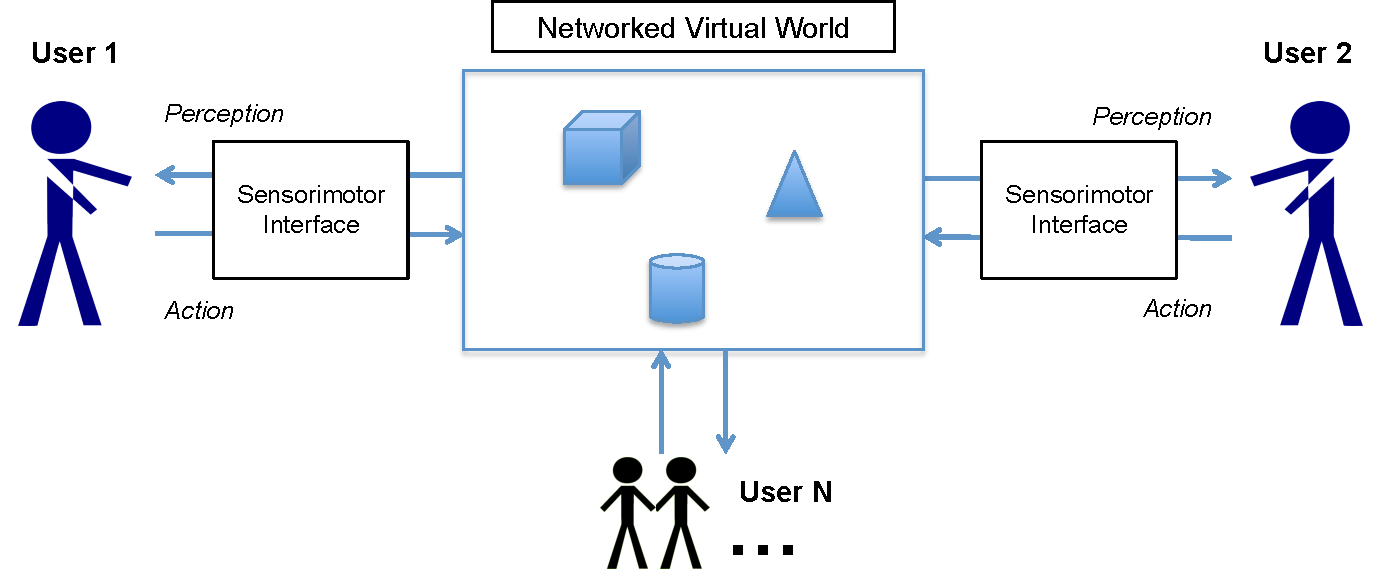
\includegraphics[width=0.9\textwidth]{figures/ch1/multi_loop}
  \caption{\label{fig:1_multi_loop}The conceptual framework of immersive CVE designed for the multi-user collaboration.}
\end{figure}

This new networked immersive experience not only changes the way people interact with objects in the virtual world, but also has impacts on how users communicate and interact with each other. The following part of this section will present in more details about different research questions and existing work around CVEs and immersive CVEs from a user-centered perspective.

\subsection{User Representation}
As discussed in section~\ref{sec:cve-issue}, users need virtual representations in the shared virtual space in order to be perceived by others. The virtual representation of users, or can be called user embodiment as explained by \citep{Benford1995Embodiment}, ``concerns the provision of users with appropriate body images so as to represent them to others (and also to themselves) in collaborative situations." Information conveyed by such representation could be position, identity, activity, availability and many other factors \citep{Thalmann2001VHR}. In an immersive virtual environment, this embodiment plays a crucial role for user interaction and communication \citep{Slater1994Body}, it is also helpful (sometimes indispensable) for users to get self-related information. For example, a user equipping an HMD perceives the virtual world from a first-person viewpoint, but his/her real body is completely blocked so a virtual body image can help to ``recreate the missing body" \citep{Lok2003Effects, Mohler2010Effect}. Moreover, according to the task that the users need to achieve in the virtual context, social representation of self may be provided through dedicated virtual clothings and/or virtual tools. 

The virtual representation of a user is usually a graphic entity, although sometimes a spatialized audio source is also sufficient for certain tasks. Three dimensional graphic recreations of human body (i.e. avatar) can be in extremely different forms, both in terms of morphology and photorealism (rendering style and Levels of Detail (LoD)) \citep{Garau2006Fidelity}. We can have from simple humanoid robots to highly detailed realistic virtual humans. For example, as shown by Figure~\ref{fig:1_vrep:rep_avatar_low}, users in MASSIVE-1 system are embodied in T-shaped robots with their names on top, they can easily get each other's information as position, orientation, identity and availability (avatars of off-line users are lying down) \citep{Greenhalgh1995MASSIVE}. Avatars as used by \citet{Roberts2004SSH} can convey more non-verbal information such as gestures and postures (Figure~\ref{fig:1_vrep:rep_avatar_high}). Users can also be represented by live video streams shown on 3D windows (billboards) \citep{Hayashi2007Immersive} (Figure~\ref{fig:1_vrep:billboard}). Another interesting method developed by \citet{Ogi2001SteAva} introduces an animated video avatar based on live video capture to avoid mesh-based avatar design. This 2.5 dimensional video avatar is captured by a set of cameras so the avatar can be seen from a certain range of directions (Figure~\ref{fig:1_vrep:video_avatar}).


\begin{figure}[htb]
  \begin{subfigure}{.5\textwidth}
    \centering
    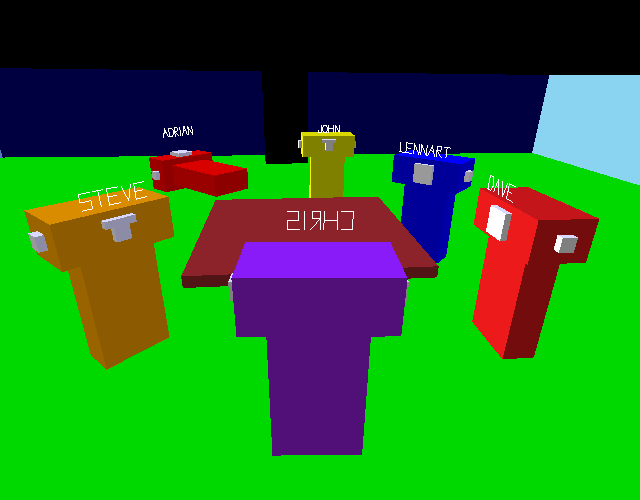
\includegraphics[width=0.9\linewidth]{figures/ch1/rep_avatar_low}
    \caption{Users represented by T-shaped robots in MASSIVE-1.}
    \label{fig:1_vrep:rep_avatar_low}
  \end{subfigure}
  \begin{subfigure}{.5\textwidth}
    \centering
    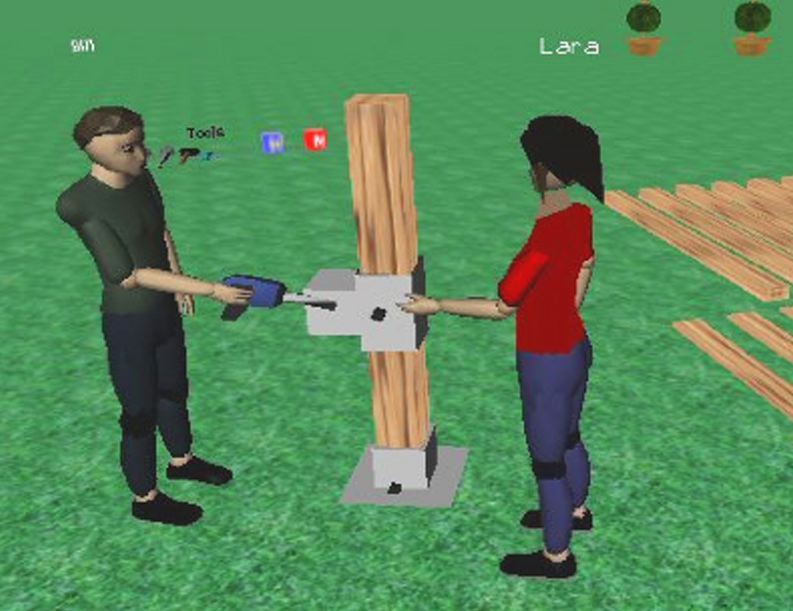
\includegraphics[width=0.9\linewidth]{figures/ch1/rep_avatar_high}
    \caption{Simple avatars with higher level of detail.}
    \label{fig:1_vrep:rep_avatar_high}
  \end{subfigure}
  \begin{subfigure}{.5\textwidth}
    \centering
    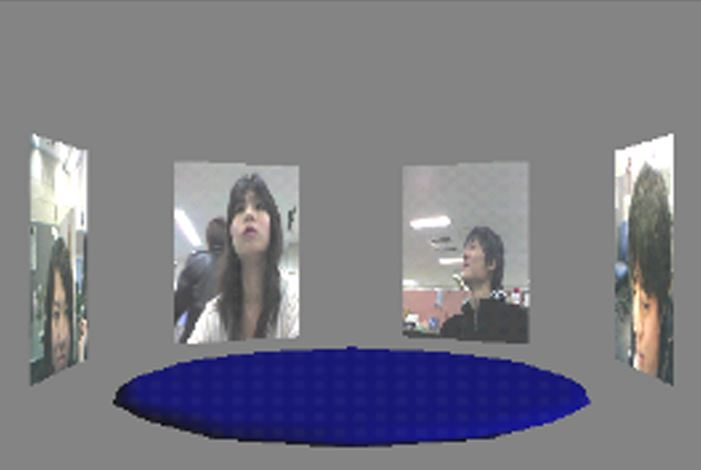
\includegraphics[width=0.9\linewidth]{figures/ch1/rep_billboard}
    \caption{Users having a round table meeting through a set of video streams shown on 3D billboard.}
    \label{fig:1_vrep:billboard}
  \end{subfigure}
  \begin{subfigure}{.5\textwidth}
    \centering
    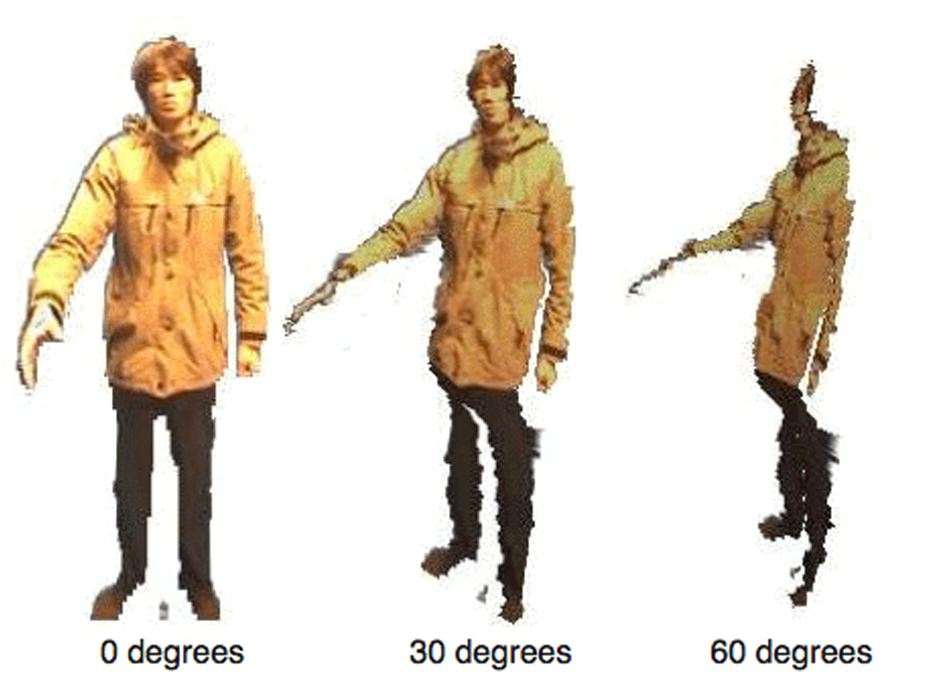
\includegraphics[width=0.9\linewidth]{figures/ch1/rep_video_avatar}
    \caption{Live video texture based 2.5 dimensional video avatar seen from various directions.}
    \label{fig:1_vrep:video_avatar}
  \end{subfigure}
  \caption{\label{fig:1_vrep} Some examples of user's virtual representation in CVEs.}
\end{figure}

In immersive CVEs (as well as desktop CVEs), high fidelity virtual humans are not always preferred against simple avatars. First, as human body is extremely complex which contains hundreds of muscles and joints, a virtual model replicating exactly the human body in real time is both challenging and costly in terms of computational and network resources. So generally we only need avatars that are ``good enough" for the given task depending on the trade-off between fidelity and efficiency. Second, the resemblance between the real user and his/her avatar is not always found to be beneficial due to the uncanny valley \citep{Mori2012Uncanny}, which has led to lots of discussions and research works in the fields of robotics and computer animation. At last, as collaborative works are task-oriented, certain tasks proceeded in non-realistic virtual worlds (e.g. scientific data visualization, imaginary artistic world) do not necessarily require virtual humans. User representations are not even limited to humanoid avatars and can be any kind of ``beings" or objects according to the context of the virtual world.

Overall, a lot of technical issues still present regarding avatar modeling, animation and motion capture technology if we look for realistic virtual humans inside immersive CVEs. \citet{Magnenat2006Interactive} give a good review of research work on interactive virtual humans in real-time virtual environments.


\subsection{User Communication}
\label{sec:user-com}
Social human communication (SHC) contains four primary elements: verbal and non-verbal communication, references to objects and references to the environment \citep{Burgoon1994Human}. \citet{Bolt1980Put}'s ``put-that-there" command gives a good illustration of these four elements despite the fact that he was talking to a computer: he was speaking (verbal communication) while pointing (non-verbal communication) to an object (reference to objects) and ``there" refers to a certain place in the virtual environment. 

When working with CVEs, references to objects and environment can be easily understood as all users share the same objects and environment. Regarding verbal and non-verbal communications, while it is relatively easy to enable direct verbal communication (spatialized audio requires more complex setup) between users, it is complicated to convey non-verbal communications through network. With desktop-based CVEs, we can play pre-recorded animations to carry out non-verbal communication as implemented in many multi-player games. However, this method is cumbersome and all personal information can not be conveyed. Immersive CVEs allow users connected by network to ``step into each other's world" and provide the closest resemblance of co-location compared to other tele-collaboration technologies \citep{Wolff2007Review}. In immersive CVEs, non-verbal cues such as gestures and postures, can be captured in real time by motion tracking and haptic devices and then replicated by avatar animation techniques.

Recent research shows increasing importance of non-verbal communications during networked collaborative work \citep{Guye1999Nonverbal, Roberts2004SSH} including gestures \citep{Dodds2011Talk}, postures \citep{Normand2012Full}, eye contact \citep{Bailenson2002Gaze, Garau2003Impact} and facial expressions \citep{Boker2009Effects}. Social scientists also start to use immersive CVEs as a tool to study human behavior in face-to-face communication by introducing biases in the virtual simulation. For example, \citet{Ennis2010Seeing} investigated human sensitivity to audio mismatches and visual desynchronization using motion capture data (Figure~\ref{fig:1_commu}). 

\begin{figure}[htb]
  \centering
  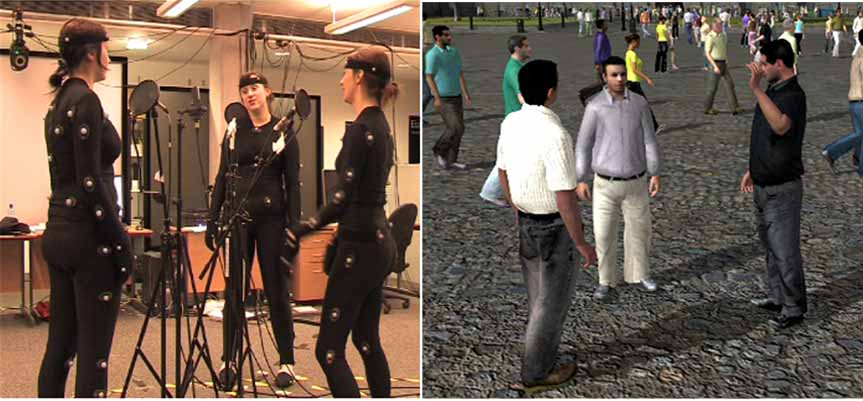
\includegraphics[width=0.9\textwidth]{figures/ch1/commu_study}
  \caption{\label{fig:1_commu} Avatars animated by motion capture data for behavioral study.}
\end{figure}

\subsection{User Interaction}
Due to the inherent differences between the real and virtual world, the way that users perform actions in the virtual world can be similar or very different from how we interact in the real world. Thus many interaction metaphors are proposed to allow users to interact (e.g. object selection and manipulation, navigation, etc.) in the virtual world as summarized by \citet{Bowman2004UIT}'s book.

During a collaborative work session, people can have similar roles and functions, e.g., two workers try to move a heavy object (\textit{piano movers' problem}), two pilots control the landing of a plane, etc. Collaborators can also have distinct roles with different associated competence, e.g. the relationship between trainer and trainee, field operator and online assistant, etc.

Closely-coupled collaboration usually involves the co-manipulation of objects between group members. Co-manipulation means that multiple users can act on the same object simultaneously, which belongs to level 3 cooperation according to \citet{Margery1999Framework}. To support object co-manipulation, the system needs to manage concurrent access to an object by combining inputs from multiple users. Two general solutions exist: we can allocate the control of different attributes to different users, i.e. separation of degrees of freedom \citep{Pinho2002Cooperative} (e.g. one moves the object while another person changes its color); if we need to modify the same attribute, for certain type of attributes (e.g. position, size, etc.) we can take the average value of all the inputs \citep{Ruddle2002Symmetric}, or we can use sophisticated metaphors for real time concurrent manipulation, such as the 3-Hand Manipulation Technique \citep{Aguerreche2009Three}, etc.

Many collaborative tasks require the cooperation among people with different profiles and skills to play different roles, like 

\citep{Pouliquen2014Role, }

\citep{Narayan2005Quantifying, Nam2008Roles, Oguz2010Haptic}



\subsection{From Presence to Co-presence}



\subsection{Summary}


\section{Conclusion}


\chapter{Co-located Collaboration with Multi-user Immersive Display}
\label{chapter:colocated_colab}
\pagebreak

\textbf{Chapter Abstract}

This chapter concentrates on how co-located users collaborate inside multi-user immersive virtual environment and it is divided into three main parts. The first presents technical aspects related to multi-user immersive displays and summarizes existing methods to separate images for different users. The second describes notions related to users' spatial organization and how users navigate in the virtual environment. Then the last part presents two major issues that we identify during the collaboration process and proposes research methodology that we adopted to solve these issues.

\vspace*{2\baselineskip}

\minitoc

\newpage
\section{Introduction}
When several users work in a multi-user immersive virtual environment for collaborative tasks, they share a virtual world on top of the same physical workspace. This physical collocation forms a mixed context which lies in the middle of \citet{Milgram1995AR}'s reality-virtuality continuum where user can have direct as well as computer-mediated interaction and communication. While lots of research works focus on supporting remote users to work efficiently together via immersive CVEs, co-located collaboration in the same immersive virtual environment for now receives limited attention. This is mainly due to the rareness and relatively high-cost of multi-user immersive systems, in contrast to non-immersive multi-user systems such as interactive walls and tables that are already widely studied in the CSCW community \citep{Scott2003System, Inkpen2005Exploring}.

Here we focus on co-located collaboration in immersive multi-user systems. Given the characteristics of collaborative work presented in chapter~\ref{chapter:context}, we are mainly interested in following research questions:

\begin{itemize}
\item How users perceive each other and achieve a shared context for collaboration?
\item How to intelligently manage users' viewpoints to support various types of collaborative tasks that require different spatial configuration of users in the virtual world (side-by-side or far away from each other)?
\item How to manage each user's workspace and spatial relationship with other users?
\item How to allow fluent transition between shared and individual activities for each user?
\end{itemize}

Below we begin by presenting multi-user immersive displays designed to offer individual stereoscopic views for multiple users. Then we talk about different concepts related to spatial arrangement of users in the common physical workspace and navigation in the virtual world. At last we talk about issues that we identified during collaborative tasks and research methods that are applied to study these issues.


\section{Multi-user Immersive Display}
Immersive display constitutes a main component of immersive virtual environment as the visual sense plays a predominant role in user's perception process. As mentioned in previous chapter (section~\ref{sec:visual_interface}), immersive displays differ from traditional displays in that they have large field of view, high resolution, stereoscopic images associated with viewpoint tracking technology.


\subsection{Stereoscopy}
\label{sec:stereo}

Stereoscopy is the production of the illusion of depth by presenting a pair of 2D images showing two perspectives that both eyes naturally have in binocular vision. Then the brain merges the two images into a ``single" one to achieve stereopsis \citep{Blake2006Perception}. Besides stereoscopy, other cues (e.g. object occlusion, linear perspective, etc.) can also help to determine relative distances and depth in a perceived scene, but stereoscopy remains the most effective factor that provides users with instant depth perception.

To achieve stereoscopic vision, we should first generate a pair of images depending on user's head position and orientation, as well as the interpupillary distance (IPD) \citep{Dodgson2004IPD}. Then we need to provide two images separately for each eye. Existing separation methods can be classified into three categories:

\begin{itemize}
\item Head-mounted displays: we can put two small screens in front of the eyes, or a single screen displaying two images side by side to show only the desired image to each eye (Figure~\ref{fig:1_vi:hmd});
\item Auto-stereoscopic screen: auto-stereoscopic display separate images at the screen level by using the lenticular lenses or parallax barrier to assure that each eye of the user sees different pixel columns which correspond to two different images \citep{Perlin2000Autostereo};
\item Eyeglasses separation: images can be separated passively by colorimetric differentiation or polarized glasses, or actively by rapidly alternating shuttered glasses.
\end{itemize}

Each type of stereoscopic display has its advantages and inconveniences. HMD is the most straightforward way to provide two different images for the eyes and allows fully visual immersion of the user (the real world is completely blocked from user's eyes except for see-through HMDs \citep{Schmalstieg2002Stube}). However, various technical limitations like limited resolution and field of view enhance user's visual fatigue and restrain the wide use of HMDs. Unlike HMDs that are heavy to carry, eyeglasses based technology combined with large immersive projection display (e.g. image wall, CAVE, dome) gives user a more comfortable stereo experience. Auto-stereoscopic screens do not require user to equip any glasses or headgear, but have limited work range - user should stay at predefined position (at a certain distance from the screen) to correctly perceive stereo images.

Recent technical developments largely improved the usability of all three types of stereoscopic display. HMDs now are lighter and less expensive with more compact design, along with better resolution, larger field of view. The improvements of immersive projection technology (IPT) \citep{Bullinger1997Immersive} makes projection-based systems with eyeglasses a widespread solution both in academic institutes and industries, and they are specially useful to create large immersive virtual environment for group immersion by the combination of multiple projectors, such as CAVEs. Auto-stereoscopic screen combined with user tracking can now allow the tracked user to pass through different viewing areas without discontinuity \citep{Kooima2010Tiled}, but still requires complex hardware and software setup. So HMDs and projection-based systems become the major platform to support immersive or partially-immersive experience.


\subsection{Visual Distortion}
Stereoscopic images are generated from a single location - the center of projection (CoP) \citep{Banks2009Perception}. A user can properly perceive the displayed 3D content on a projection screen when viewed from the CoP. So in an immersive virtual environment, user's viewpoint is captured by head-tracking to serve as the CoP to generate appropriate images in real time as the user moves physically.

While HMDs provide personal stereoscopic images for a single user, projection-based systems are often shared by a group of people for team work, as shown by Figure~\ref{fig:2_group}. In such multi-user situation, only the tracked user receives correct stereo images from the CoP, other co-located users (followers) share the same stereo images intended for the tracked user and participate passively in the collaborative task \citep{Bayon2006Multiple}. When users are close enough to the tracked user, they can get a relatively faithful representation of the virtual environment, but as the distance increases, displacement from the CoP results in increasingly inappropriate stereo cues and distorted perception of the virtual space.

\begin{figure}[htb]
  \centering
  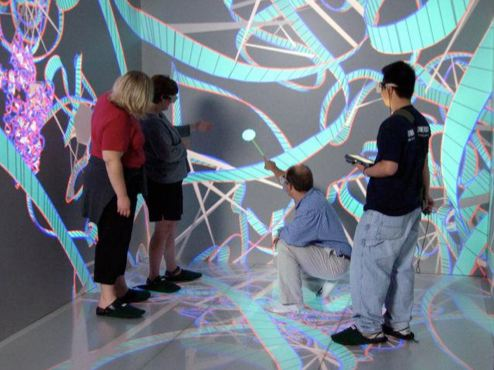
\includegraphics[width=0.6\textwidth]{figures/ch2/group}
  \caption{\label{fig:2_group}A group of people collaborating in a CAVE for data visualization \citep{Pollock2012Right}.}
\end{figure}

\begin{figure}[htb]
  \centering
  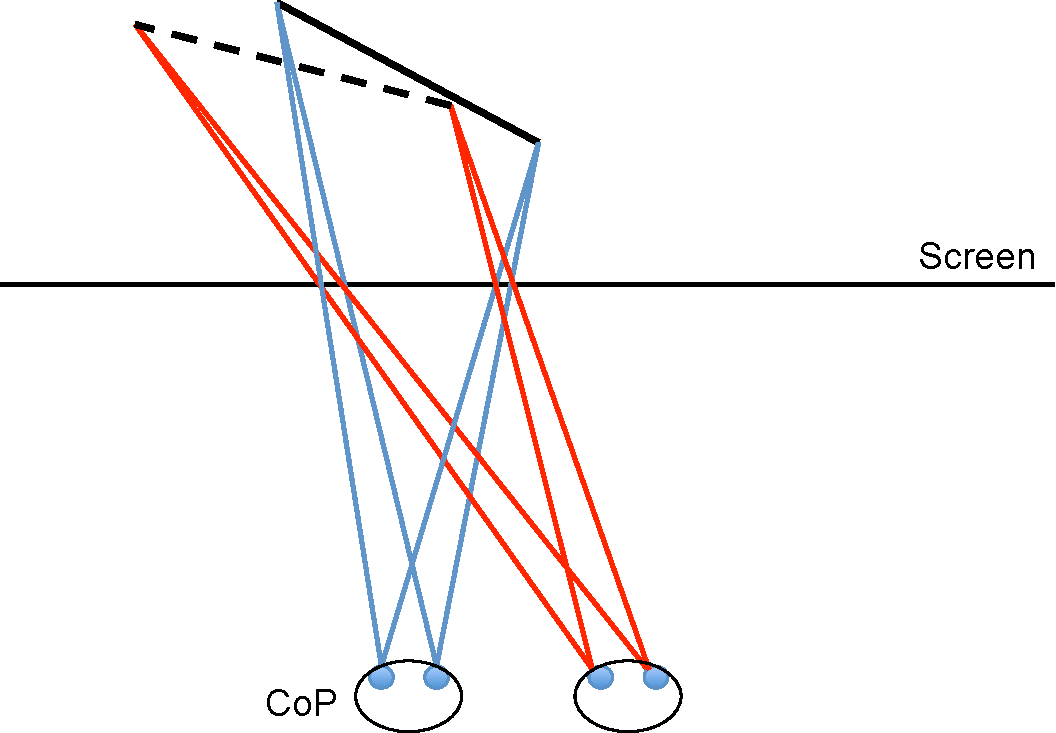
\includegraphics[width=0.48\textwidth]{figures/ch2/distortion_1}
  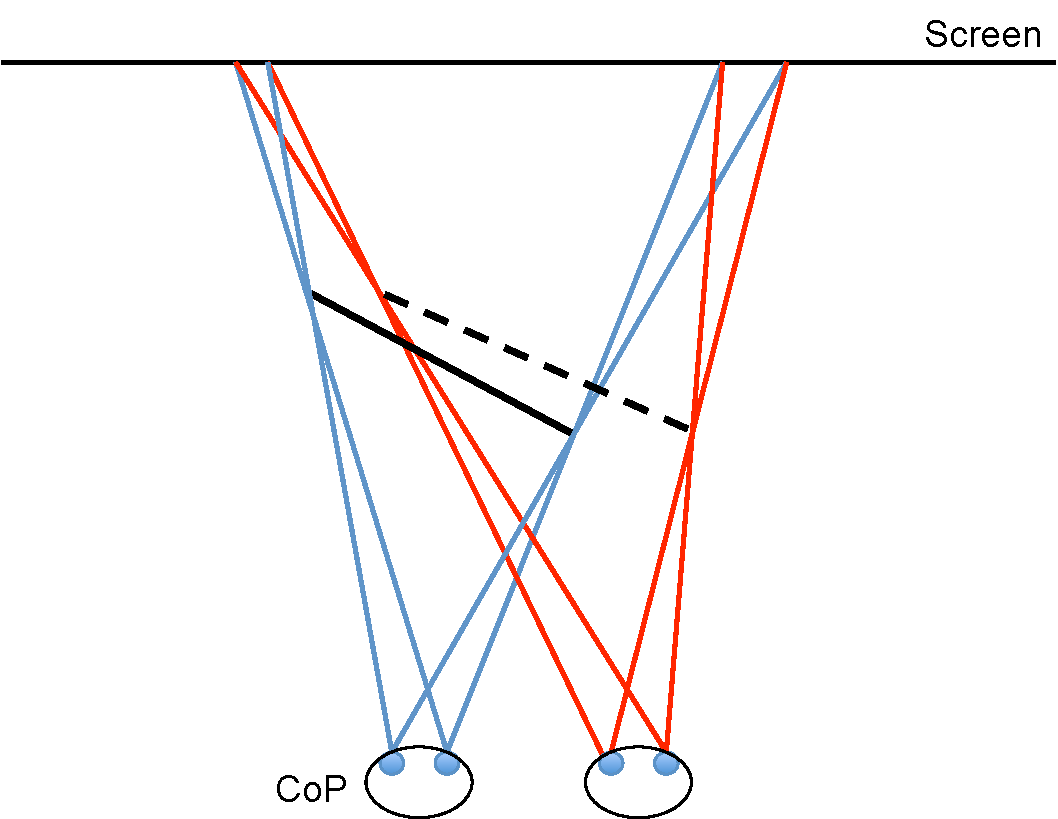
\includegraphics[width=0.48\textwidth]{figures/ch2/distortion_2}
  \caption{\label{fig:2_ray_model}Illustration of visual distortion by perceiving the right view from a location other than the CoP. The black line represents the correct view of object perceived from CoP and the dotted line corresponds the distorted view observed from another location.}
\end{figure}


Visual distortion caused by displacement from the CoP can be predicted by a ray-intersection model \citep{Burton2012Diagnosing}. As shown by Figure~\ref{fig:2_ray_model}, no matter the virtual object is situated behind or in front of the screen, a lateral displacement from the CoP will cause deformation and shift of the perceived object. Similar effects can be observed by moving forward or backward with respect to the CoP.

A series of studies have been conducted to assess the influences of such visual distortion. When viewing monocular displays from locations displaced from the CoP, the spatial judgments remain relatively acceptable. \citet{Vishwanath2005Pictures} investigated the mechanism underlying this perceptual invariance by studying the perceived shapes of pictured objects viewed from various locations and they find that invariance is achieved through the awareness of the 2D picture plane. However, when it comes to stereo images, \citet{Banks2009Perception}'s experiment indicates that human viewers of stereo pictures are unable to compensate for incorrect viewing position. This result is confirmed by follow-up studies: judgments of angles are distorted after leftward and rightward displacement from the CoP \citep{Burton2012Diagnosing} and judgments of object depth are distorted after forward and backward displacement from the CoP \citep{Pollock2012Right}, although the magnitude of these distortions is consistently less than predicted by the ray-intersection models. More studies on visual distortions in stereoscopic systems can be found in articles by \citet{Woods1993Image, Held2008Misperceptions, Ponto2013Perceptual}.


\subsection{View Separation}
To better support co-located use of immersive virtual environments, we need to provide perspective-correct (distortion free) individual stereoscopic views for each user. One direct way is to use personal displays such as HMDs \citep{Salzmann2008TUS} or see-through HMDs \citep{Schmalstieg2002Stube}, and another solution is to introduce adaptations to existing immersive displays which already support group immersion.

\citet{Bolas2004New} categorize solutions for displaying multiple images in a common area:

\begin{itemize}
\item Spatial barriers use the display's physical configuration and user placement to block users from seeing each other's view.
\item Optical filtering involves systems that filter viewpoints using light's electromagnetic properties, such as polarization or wavelength.
\item Optical routing uses the angle-sensitive optical characteristics of certain materials to direct or occlude images based on the user's position.
\item Time multiplexing solutions use time-sequenced light and shutters to determine which user sees an image at a given point in time.
\end{itemize}

Except the first solution, the three other options are the same technologies that are used to separate images for the left and right eye of a single user as presented in section~\ref{sec:stereo}. Multi-user systems are often build with mixed solutions from these categories, here is a description of existing systems that provide independent stereo images for different users inside immersive or semi-immersive environment.


\subsubsection{Image Separation} 
Typically we can create separate image channels for different users by adding shutters and/or optical filters in front of projectors combined with synchronized counterparts in front of user's eyes.

The two-user Responsive Workbench developed by \citet{Agrawala1997TRW} relies purely on a time-multiplexing method which displays four different images in sequence on a CRT projector at 144Hz, thus each eye of a user views the virtual scene at 36Hz (Figure~\ref{fig:2_sep_active:wb}). This workbench is the first demonstration of a two-user stereoscopic system, but the time-multiplexing method largely reduces projection time for each eye (low brightness) and users suffer from image flicker and crosstalk. \citet{Blom2002Multiple} then extended this active shuttering method to multi-screen systems like CAVEs. \citep{Froehlich2004Implementing} further studied active shuttering technology by testing two kinds of shutters on the projector side with a range of shuttering frequencies (Figure~\ref{fig:2_sep_active:four}). The mechanical shuttering delivers higher brightness and less cross talk, but does not extend as easily to more than two users as liquid crystal (LC) shutters because of the required rotation speed and size of the disc. They tested LC shutters from 140Hz to 400Hz and found that users did not perceive flicker above a refresh rate of 200Hz, but a frequency higher than 320Hz would result in very dark images.

\begin{figure}[htb]
  \begin{subfigure}{.5\textwidth}
    \centering
    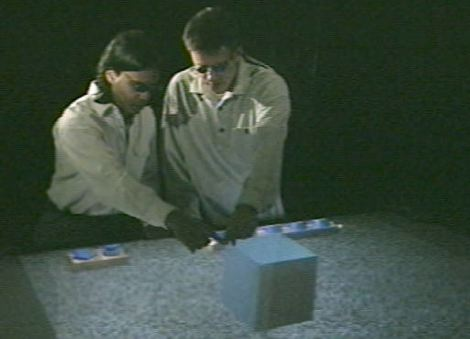
\includegraphics[height=5cm]{figures/ch2/resp_workbench}
    \caption{The two-user Responsive Workbench.}
    \label{fig:2_sep_active:wb}
  \end{subfigure}
  \begin{subfigure}{.5\textwidth}
    \centering
    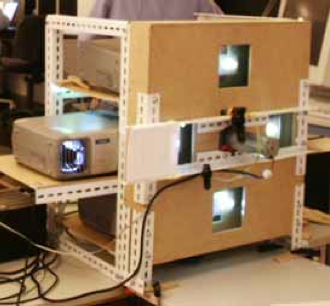
\includegraphics[height=5cm]{figures/ch2/four_proj}
    \caption{Two-user active separation with four projectors.}
    \label{fig:2_sep_active:four}
  \end{subfigure}
  \caption{\label{fig:2_sep_active}User separation by time-multiplexing with active shutters.}
\end{figure}

\begin{figure}[htb]
  \begin{subfigure}{.5\textwidth}
    \centering
    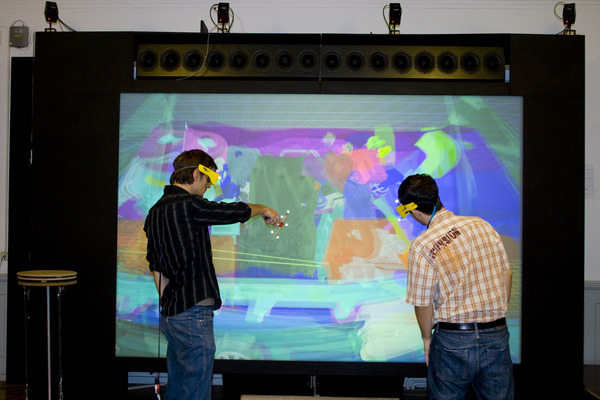
\includegraphics[width=\linewidth]{figures/ch2/multiview_wall}
    \caption{Wall display for two users.}
    \label{fig:2_sep_active_passive:wall}
  \end{subfigure}
  \begin{subfigure}{.5\textwidth}
    \centering
    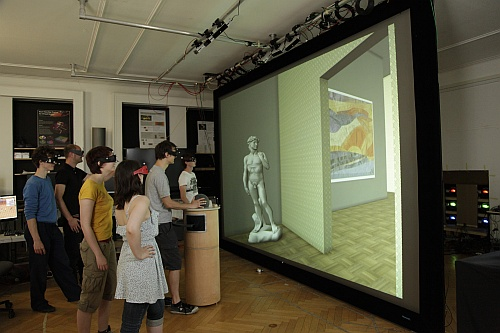
\includegraphics[width=\linewidth]{figures/ch2/C1x6}
    \caption{The six-user projection wall display.}
    \label{fig:2_sep_active_passive:6user}
  \end{subfigure}
  \caption{\label{fig:2_sep_active_passive}User separation by active time-multiplexing combined with polarization.}
\end{figure}

Another solution is to combine time-multiplexing with polarization filters. In 1999, Barco developed the ``Virtual Surgery Table"\footnote{http://www.barco.com/en/Products/Compact-Multi-User-Projection-Table.aspx/} which provides two users with stereoscopic images by differently polarizing the output of two active stereo projectors. Then \citet{Frohlich2005MultiViewer} extended this shuttered display to support up to four users with eight shuttered liquid-crystal display (LCD) projectors (Figure~\ref{fig:2_sep_active_passive:wall}). In this setup, images for different users are separated by active shutter glasses while the separation of the images for the left and right eye is ensured by passive polarized filters. This approach shows better performance in terms of perceived flicker, brightness of each view and crosstalk compared to purely active shuttering method.


\citet{Frohlich2005MultiViewer} also summarized three main parameters can be considered to evaluate the quality of a multi-stereoscopic projection system:

\begin{itemize}
\item Brightness per view;
\item Static and dynamic crosstalk; 
\item Perceived flicker, which depends on the shutter frequency, the video rate of the projector and brightness.
\end{itemize}

In 2011, \citet{Kulik2011CSS} developed a projection-based stereoscopic display for six users by using six customized digital light processing (DLP) projectors running at 360Hz for a single screen, which results in 60Hz per user (Figure~\ref{fig:2_sep_active_passive:6user}).


\citet{Dodgson2005Autostereoscopic} provided an introduction and overview of auto-stereoscopic multi-view displays. Users in this kind of multi-view system get perceive 3D objects from his/her own point of view without tracking or eyeglasses, but only inside a limited zone depending on different properties of the display. Another issue is that with increasing number of views (e.g. up to 256 views by \citet{Takaki2010Multi}), generating images in real time for dynamic interaction would be a challenge.

\subsubsection{Spatial Separation}
Instead of creating image channels, we can also take advantage of the spatial property of the display by assigning different screens or parts of a single screen to different users. For example, the ``Protein Interactive Theater" (PIT) \citep{Arthur1998PIT} uses two orthogonal screens and each user looks at only one of the screens (Figure~\ref{fig:2_sep_spatial:pit}). The IllusionHole \citep{Kitamura2001Interactive} uses a circular mask on top of a tabletop projection. By looking through the mask, users positioned around the table see their individual stereo images shown in different areas of the screen (Figure~\ref{fig:2_sep_spatial:illu}). Other systems like the Virtual Showcase \citep{Bimber2006Virtual}and Joint Space Station \citep{Mulder2004Modular} use similar mirror-based display to support multiple users. These desktop-based systems are often designed to accomplish specific collaborative tasks (e.g. 3D object visualization) and provide limited workspace with inherent spatial constrains. 

\begin{figure}[htb]
  \begin{subfigure}{.45\textwidth}
    \centering
    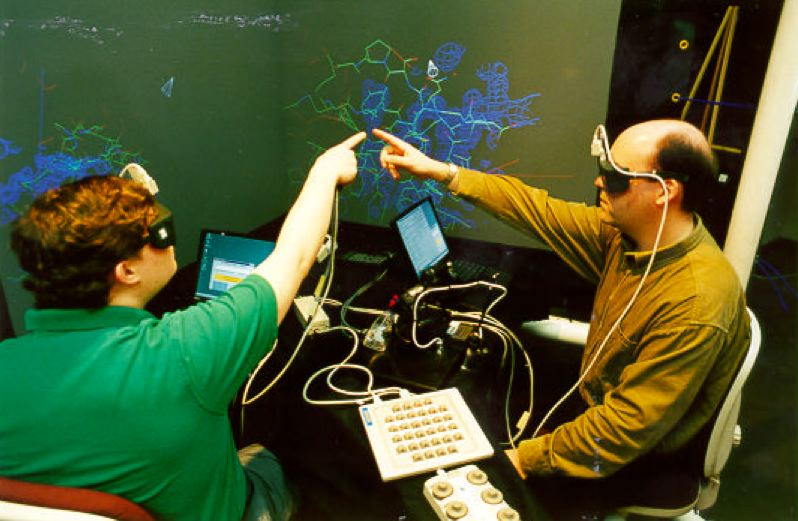
\includegraphics[height=4.5cm]{figures/ch2/pit}
    \caption{The PIT system for two-user collaboration.}
    \label{fig:2_sep_spatial:pit}
  \end{subfigure}
  \begin{subfigure}{.55\textwidth}
    \centering
    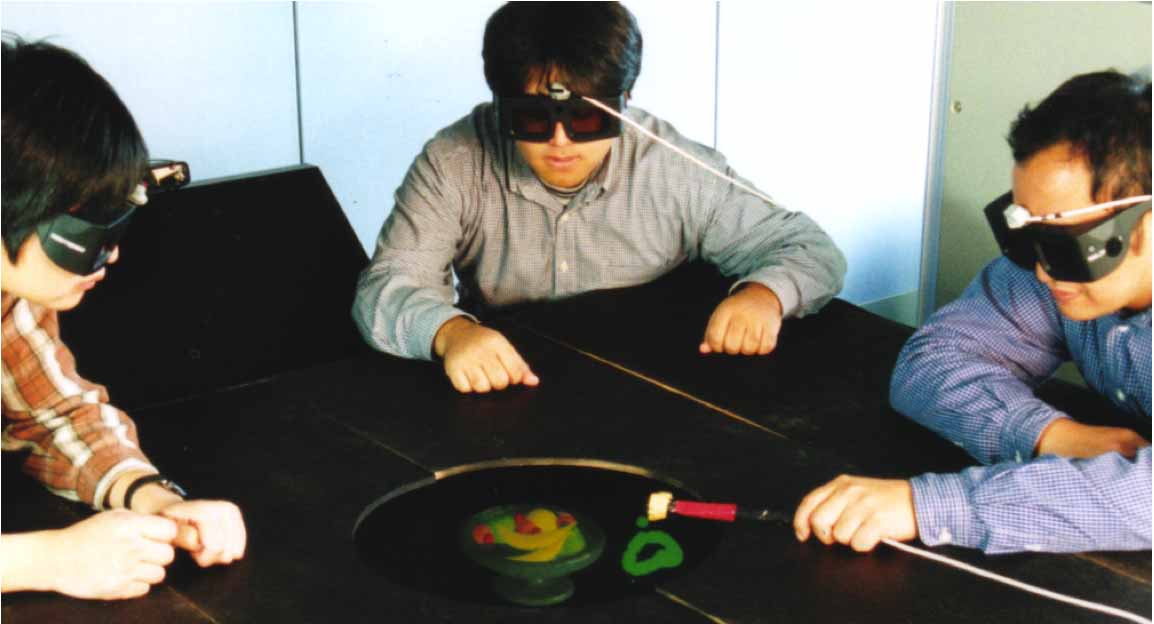
\includegraphics[height=4.5cm]{figures/ch2/illusionHole}
    \caption{The IllusionHole for tabletop collaboration.}
    \label{fig:2_sep_spatial:illu}
  \end{subfigure}
  \caption{\label{fig:2_sep_spatial}User separation by using different screens or different parts of the same screen.}
\end{figure}

When using larger wall display or CAVE, users can have head-tracked individual monoscopic \citep{Maksakov2010Whale} or stereoscopic views \citep{Schulze2012Democratizing} on different parts of the display. When they share the same part of the screen, sophisticated algorithms are applied to recalculates images based on an averaged viewpoint depending on positions and orientations of all tracked users. These software-based solutions allow co-located collaboration in immersive virtual environment without additional hardware setup, although the reduced visual distortions could still be disturbing for certain tasks that require precise spatial operations (e.g. object co-manipulation).

\subsubsection{Other Methods}
There are also many other display solutions offering individual stereoscopic views like the volumetric display \citep{Grossman2008Volum} and holographic display \citep{Lucente1997Holo}. However, for now it is still difficult to extend these displays to provide large-scale visual immersion. 

Another interesting multi-user display is the omni-stereo display \citep{Simon2004Omni} such as AVIE \citep{Mcginity2007Avie} and i-Cone \citep{Simon2002Icone} which provides good support for immersive visualization with large user group, but theoretically users need to stay at predefined positions to get good perspective. \citet{Simon2007MVI} compared usability and interaction performance between multi-viewpoint images and head-tracked stereo display. Results showed that for certain tasks that users do not need to move physically (e.g. ray-casting selection and in-hand object manipulation), multi-viewpoint images can produce similar or even better performance than fully head-tracked interaction.


\subsection{Summary}
This section gives a general presentation of multi-user immersive display from the initial motivation (to provide distortion-free stereoscopic view for each user) to various implementations.

Among all presented multi-user display technologies, the active \& passive method which combines time-multiplexing with polarization filters is the most effective and cost-efficient way to build multi-user immersive virtual environment. There are multiple reasons: first, it completely eliminated visual distortion due to observation from another position than the CoP; second,
it can be easily applied to different shapes of large-scale immersive systems like walls, CAVEs or domes without imposing strong spatial constrains on user's position and orientation with respect to the screen(s), users can move inside a relatively large physical workspace; at last, compared to purely time-multiplexing separation, it provides high brightness, low crosstalk and less flicker stereo images.   

% -------------------------------------------------------------------------------------------------


\section{Spatial Organization} 

\subsection{Stage}
\label{sec:stage}
In most VR systems, there is a spatial reference frame that maps user's physical position in the tracking space to a corresponding location in the virtual world, so that the computer can use this position to render proper images in correspondence with user's point of view. In practice, the spatial reference frame is often expressed as the virtual coordinates of the center of physical workspace defined by the screen and/or tracking device configuration. Here we borrow some definitions from the Immersive Interactive Virtual Cabin (IIVC) model (Figure~\ref{fig:2_iivc}) that can help to describe user's workspace:

\begin{itemize}
\item The \textit{stage} is a virtual representation of the physical workspace;
\item The \textit{conveyor} is the integration frame of the stage into the virtual world. This conveyor has its own position, orientation and scale in the virtual world coordinate system, and the stage is linked to the conveyor with position, orientation, and scale offsets.
-\end{itemize}

\begin{figure}[htb]
  \centering
  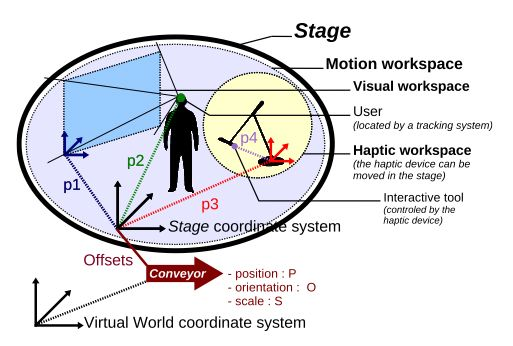
\includegraphics[width=.7\textwidth]{figures/ch2/IIVC}
  \caption{\label{fig:2_iivc}The IIVC model: the conveyor carries the stage with its workspaces in the virtual world \citep{Fleury2010Generic}.}
\end{figure}

So with the stage model, the stage center becomes the spatial reference frame to correctly locate not only the user, but also other devices (e.g. props) in the virtual world. For example in Figure~\ref{fig:2_reference}, from left to right, user remains at the same position in the physical workspace while the stage center is set to different location in the virtual world, the user will have different virtual viewpoints accordingly.

\begin{figure}[htb]
  \centering
  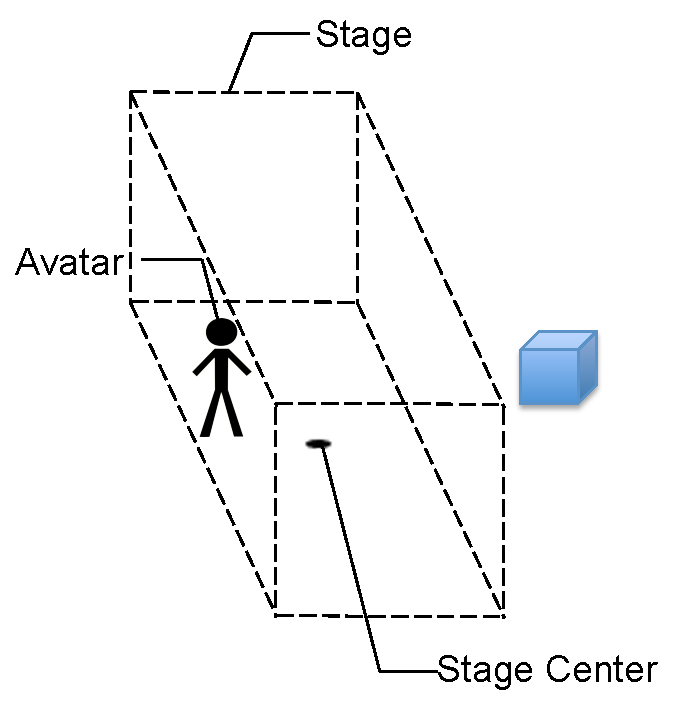
\includegraphics[width=.4\textwidth]{figures/ch2/referenceframe_1}
  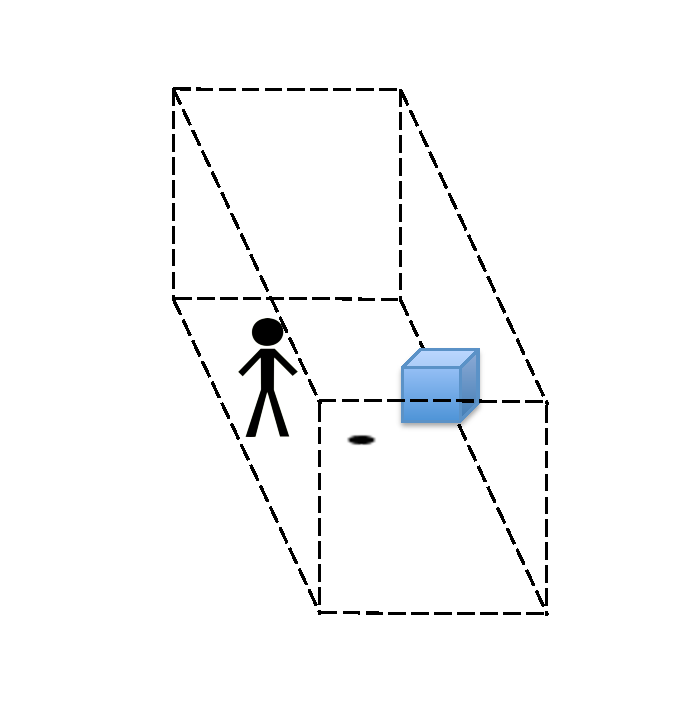
\includegraphics[width=.4\textwidth]{figures/ch2/referenceframe_2}
  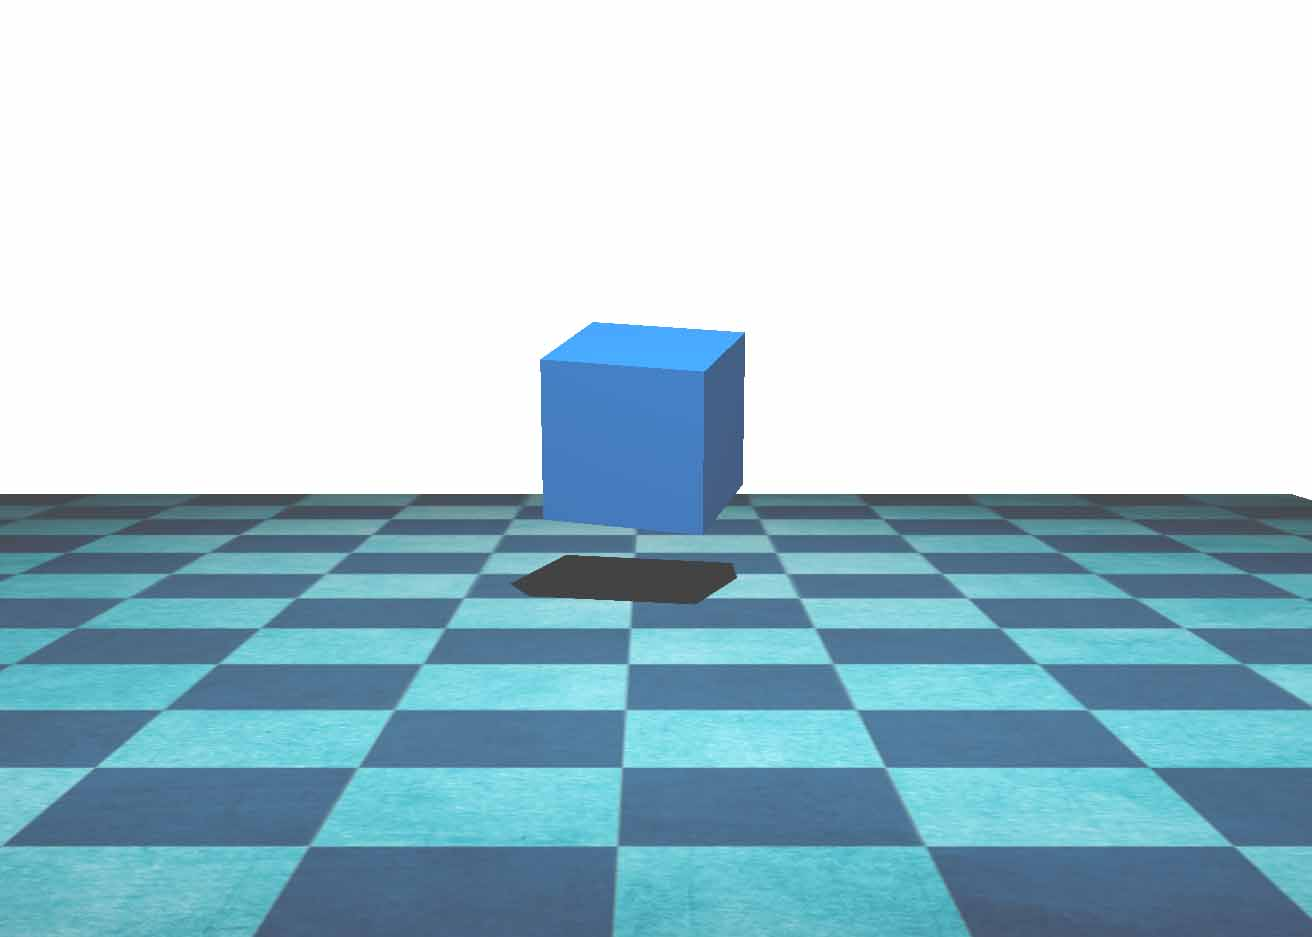
\includegraphics[width=0.48\textwidth]{figures/ch2/ref_1}
  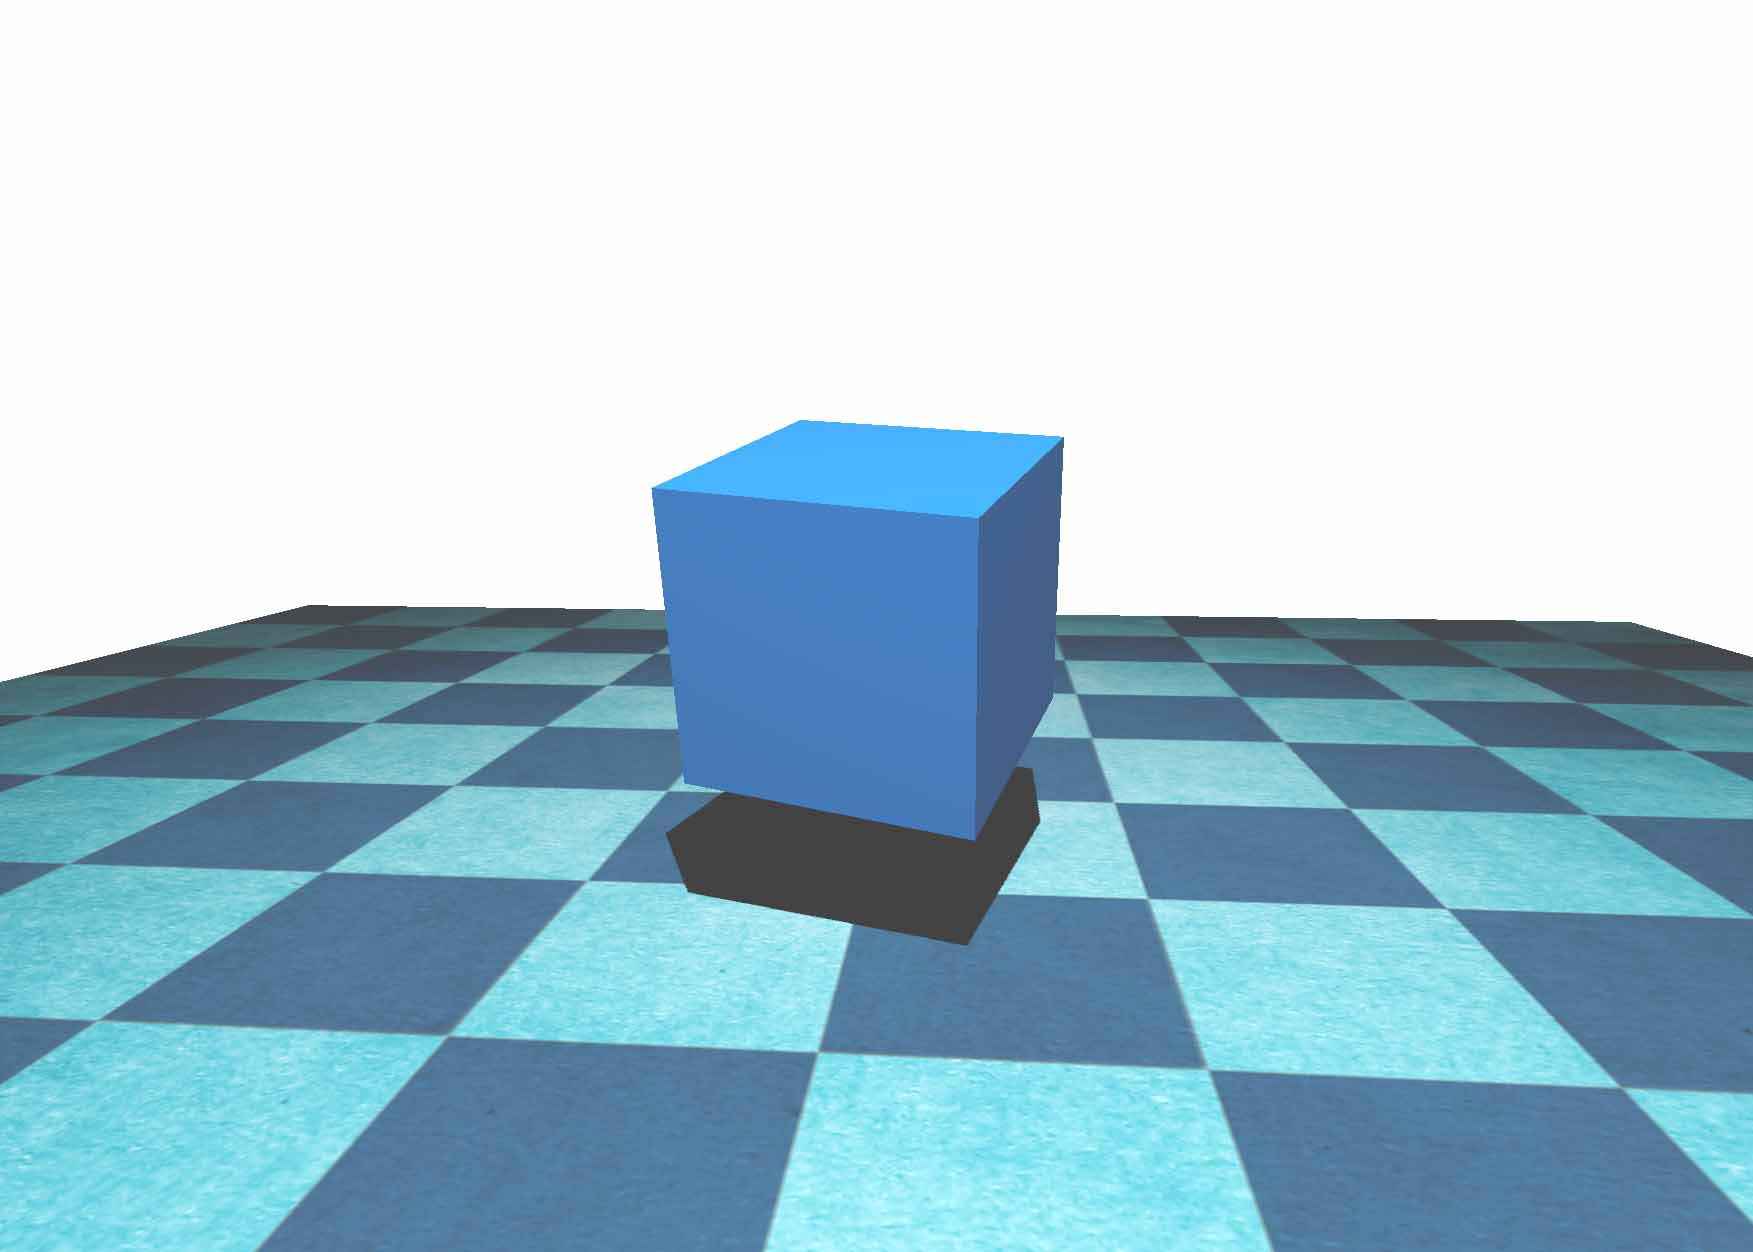
\includegraphics[width=0.48\textwidth]{figures/ch2/ref_2}
  \caption{\label{fig:2_reference}Illustration of the impact of moving spatial reference frame on user's viewpoint location in the virtual scene.}
\end{figure}

\subsection{Spatial Consistency}
In a multi-user virtual environment, each user has a corresponding stage in the virtual world. The multi-user display system is able to render completely different stereoscopic images for each user depending on the configuration of users' stage centers.

When all stage centers are strictly superimposed, the spatial relationship between users in the virtual world will be consistent with their relative spatial distribution in the real workspace. In an immersive multi-user virtual environment, this spatial consistency allows users to perceive a virtual object at exactly the same physical location from corresponding viewpoints (Figure~\ref{fig:2_consistency} top). This particular situation is quite similar to cases when users collaborate around physical objects in the real world.

Otherwise, each user will no longer perceive the same object at the same physical location. What a user perceives totally depends on the configuration of spatial reference frame in the virtual world. For example in bottom part of Figure~\ref{fig:2_consistency}, user B's stage center is shifted to the left regarding the one of user A, so user B sees a cube in front of him/her while user A considers the same cube to be on user B's left.

\begin{figure}[htb]
  \centering
  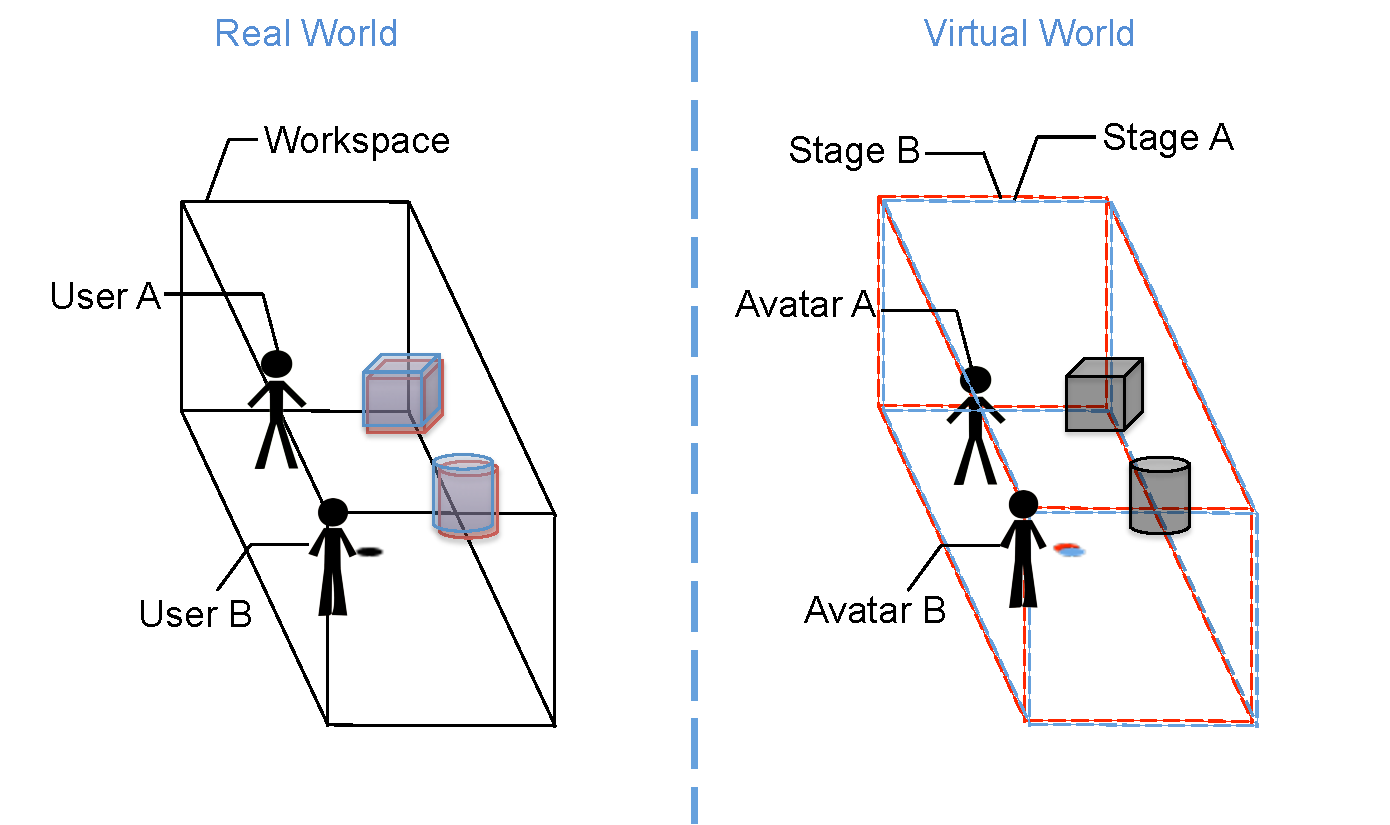
\includegraphics[width=.7\textwidth]{figures/ch2/consistency_1}
  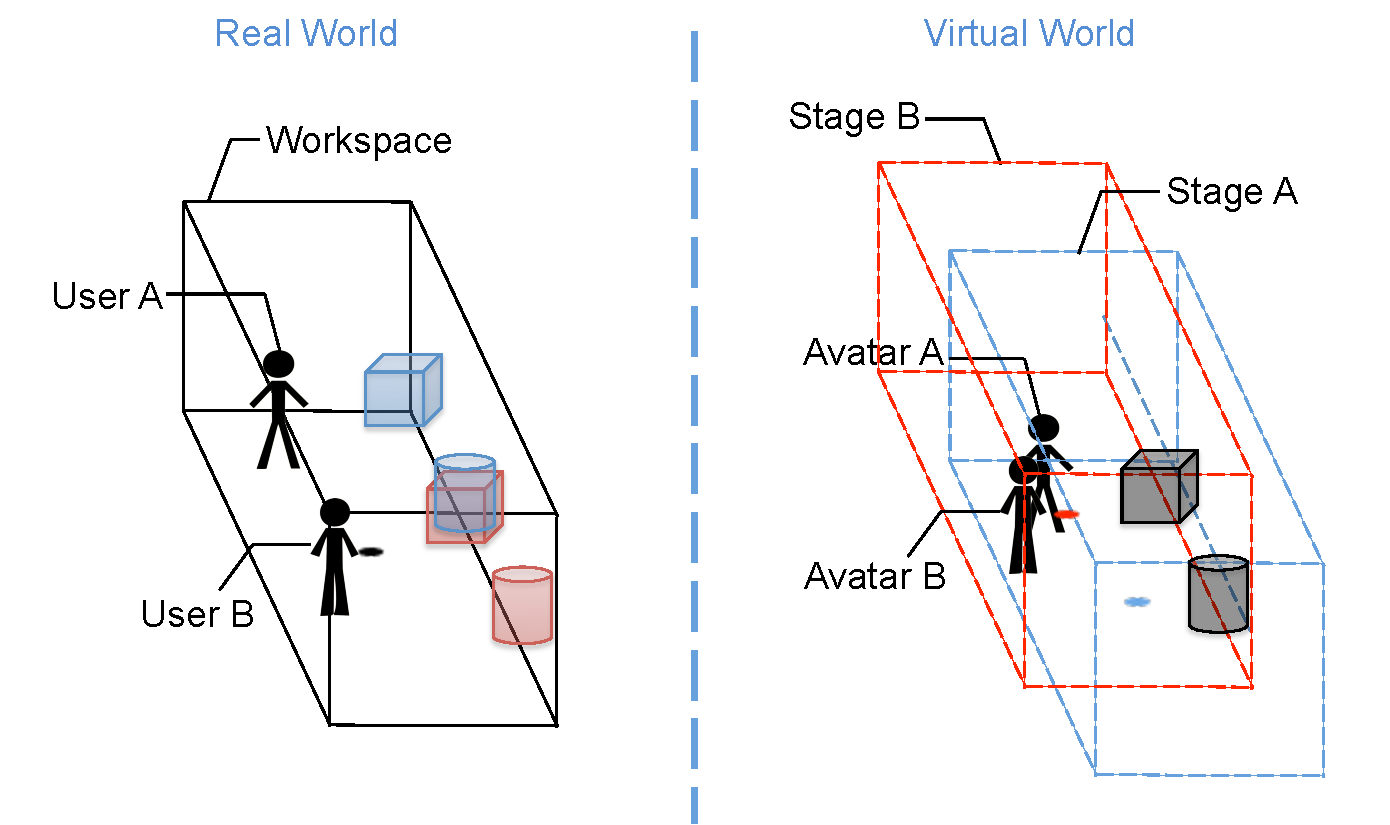
\includegraphics[width=.7\textwidth]{figures/ch2/consistency_2}
  \caption{\label{fig:2_consistency}Distribution of users' stage centers: consistent mode (above) and individual mode (below).}
\end{figure}


\subsection{Collaborative Mode}
The distribution of stage centers has a direct influence on how users interact and communicate with each other, so collaboration in multi-user immersive virtual environment can be divided into two modes depending on whether the spatial consistency is maintained among all the users.


\subsubsection{Consistent Mode}
In this mode, all users' virtual spaces are consistent with the common physical workspace which result in a shared spatial understanding of the virtual environment. In this context, users can communicate spatial information similarly as in the real world. For example, one can speak to another ``Pass me the book on your left", or point to objects or directions by deictic gestures \citep{Salzmann2009VRPointing} (Figure~\ref{fig:2_consistent_collab:pointing}). Another advantage of consistent mode is that users can make use of tangible devices (props) to get passive tactile feedback for object co-manipulation \citep{Aguerreche2009Three, Salzmann2009CIC} (Figure~\ref{fig:2_consistent_collab:tangible}) or for other specific tasks like two-user driving test \citep{Salzmann2008TUS}, etc.

In projection-based immersive system, we can consider that users' physical bodies are directly ``integrated" into the virtual environment. Social cues that facilitate human communication (e.g. gestures, postures, facial expressions and gaze direction, etc.) can be conveyed without computer mediation. This is a big advantage compared to remote situations where users communicate through embodied avatars. 

\begin{figure}[htb]
  \begin{subfigure}{.3\textwidth}
    \centering
    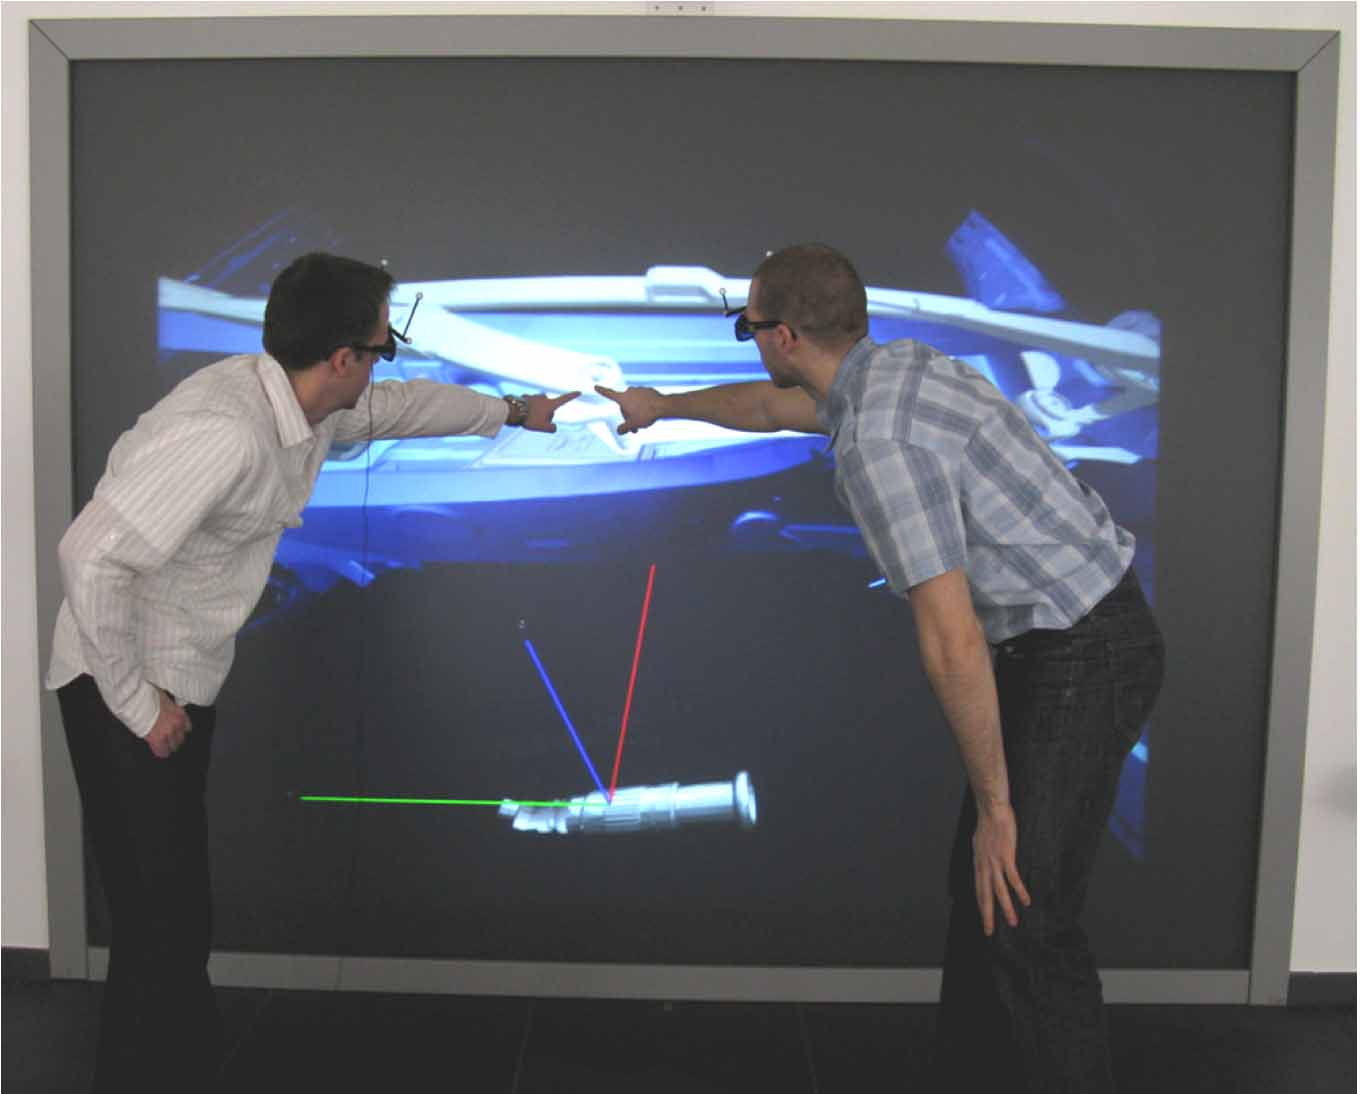
\includegraphics[width=\linewidth]{figures/ch2/pointing}
    \caption{Direct user interaction with deictic gestures.}
    \label{fig:2_consistent_collab:pointing}
  \end{subfigure}
  \begin{subfigure}{.7\textwidth}
    \centering
    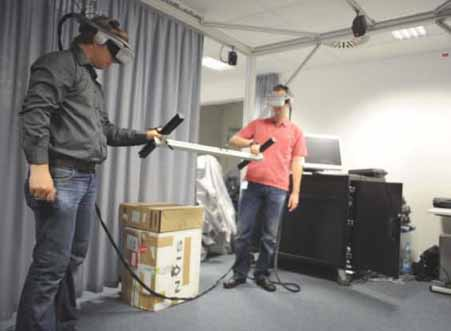
\includegraphics[height=4cm]{figures/ch2/tangible_1}
    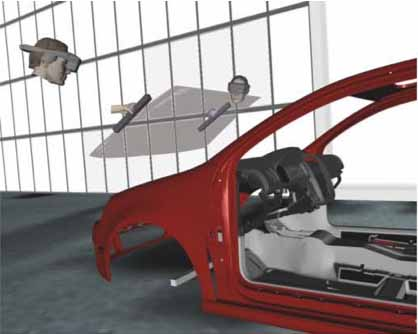
\includegraphics[height=4cm]{figures/ch2/tangible_2}
    \caption{A windshield assembly task using tangible interface.}
    \label{fig:2_consistent_collab:tangible}
  \end{subfigure}
  \begin{subfigure}{.45\textwidth}
    \centering
    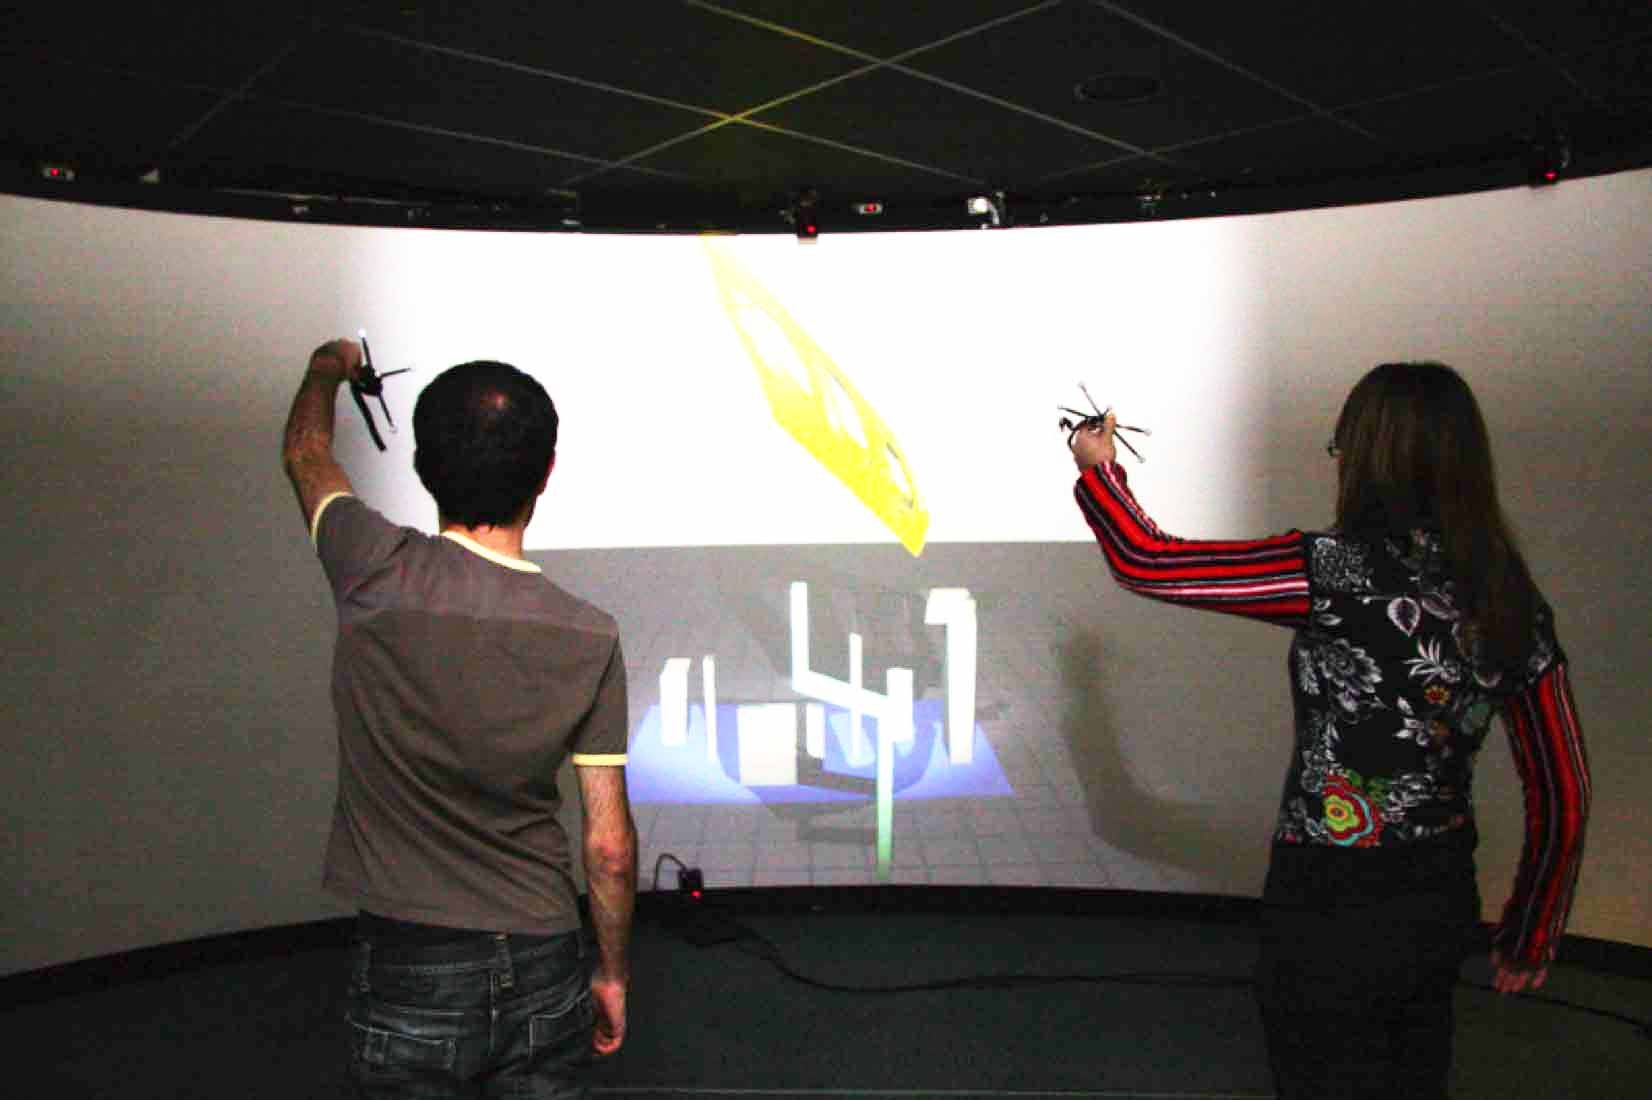
\includegraphics[height=4.6cm]{figures/ch2/comanip}
    \caption{Object co-manipulation with flysticks.}
    \label{fig:2_consistent_collab:comanip}
  \end{subfigure}
  \begin{subfigure}{.55\textwidth}
    \centering
    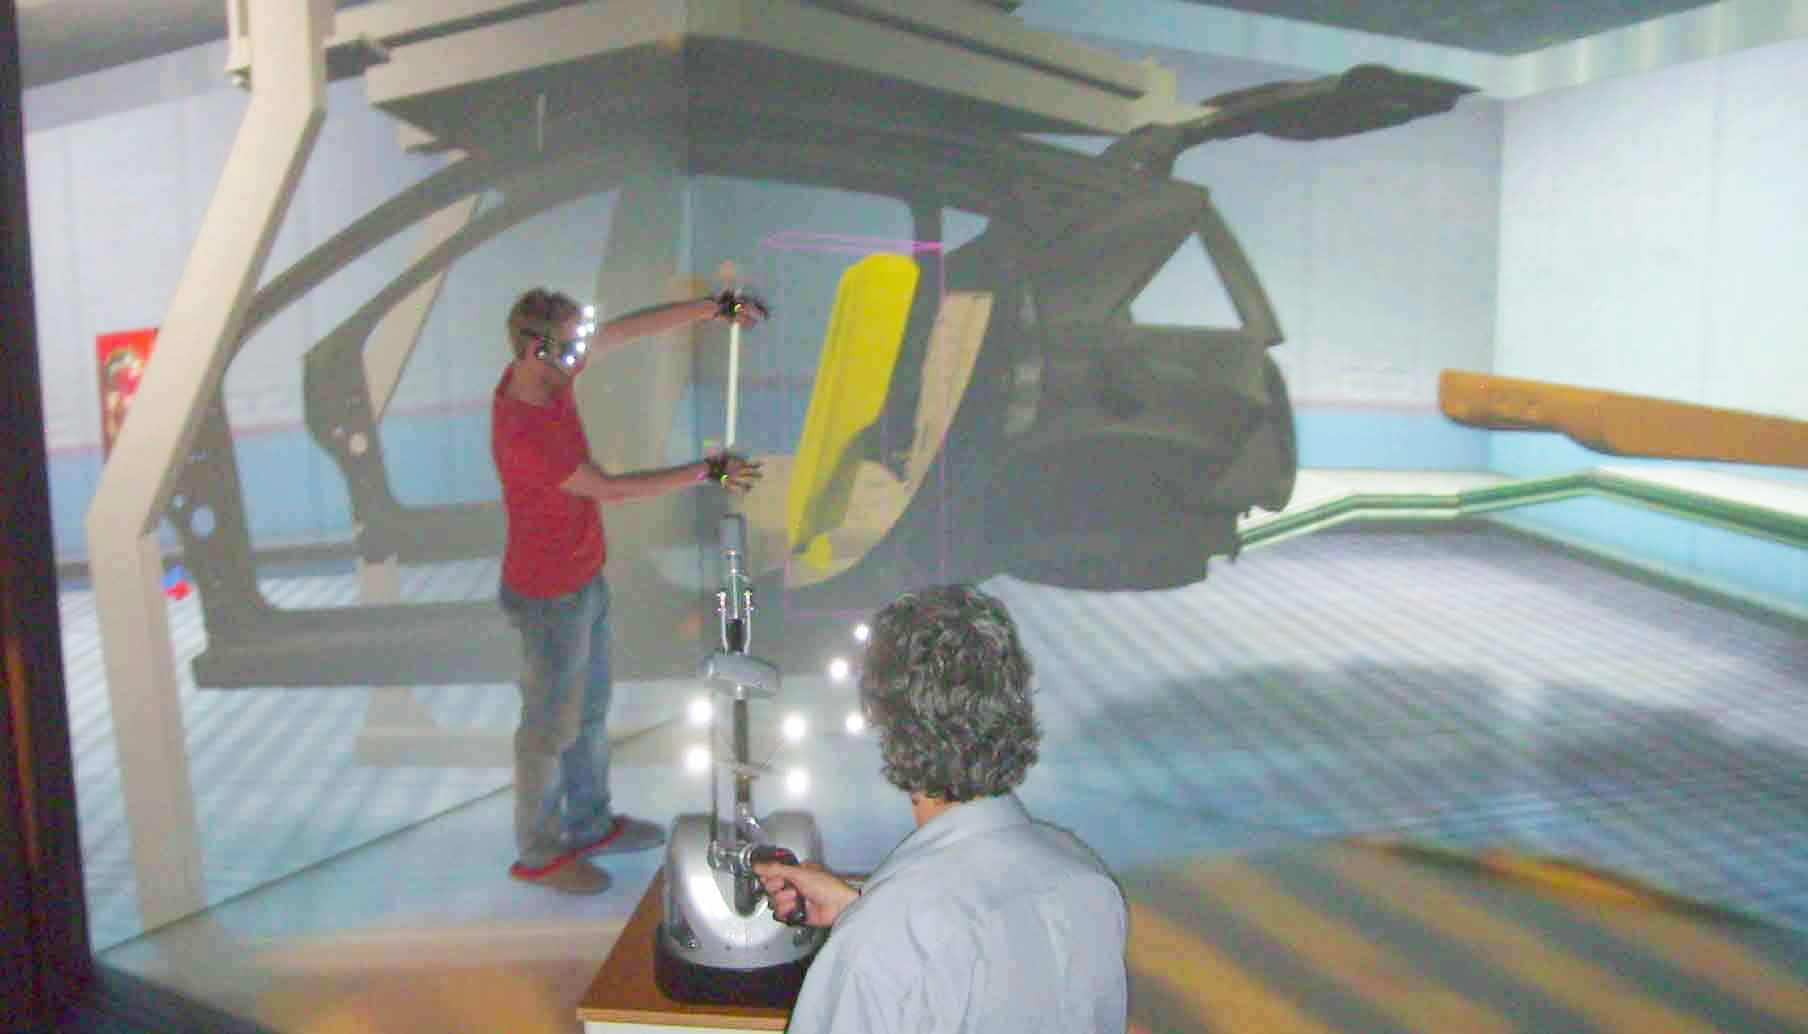
\includegraphics[height=4.6cm]{figures/ch2/malcomiics}
    \caption{MalCoMIICs demo for car assembly task.}
    \label{fig:2_consistent_collab:malcomiics}
  \end{subfigure}
  \caption{\label{fig:2_consistent_collab}Co-located collaborations in consistent mode.}
\end{figure}

The consistent mode is initially motivated by efforts to bring distortion-free stereoscopic view for each tracked user, and for a long time it is considered to be the default mode for co-located collaboration. This consistent mode suits well for closely-coupled collaborative tasks \citep{Simon2005First, Aguerreche2010Comparison, Martin2011Reconfigurable} (Figure~\ref{fig:2_consistent_collab:comanip} and \ref{fig:2_consistent_collab:malcomiics}) that do not require users to be or travel to different virtual places.

However, this spatial constrain restricts collaborative scenarios that can be supported in multi-user immersive virtual environment. Though several interaction techniques have been proposed to get around spatial constrains and to extend collaborative scenarios in consistent mode, such as the bent pick ray \citep{Riege2006Bent} and the see-through techniques \citep{Argelaguet2010STT}.

\subsubsection{Individual Mode}
As opposite to consistent mode, the individual mode loosens constrains applied to users' stage centers. This mode is complementary to the consistent mode and largely broadens collaborative scenarios that can be supported in the co-located use of immersive virtual environment. Collaborative scenarios can be extended in the following ways:

\begin{itemize}
\item Spatial distribution of users in the virtual world becomes more flexible:
\begin{itemize}
  \item Users are distributed at remote virtual places;
  \item Users are situated in a virtual space larger than the available physical workspace;
  \item Users are close to each other around an object of interest, but from different perspectives that they can get in consistent mode;
\end{itemize}
\item Artificial control of users' viewpoints:
\begin{itemize}
  \item To provide user with a third-person view or a god view of the virtual scene;
  \item To enable multi-scale observation (zoom on a particular zone);
  \item To quickly share one's first person view to others, or to exchange viewpoints between users \citep{Lopez2014Exchange}.
\end{itemize}
\end{itemize}

The individual mode can be very useful, even indispensable in some cases. For example, when two users working face-to-face in a projection-based immersive system, objects situated between them can not be correctly perceived since images on the screen are occluded by user's body. In this case individual mode can be applied to allow users to be virtually face-to-face while being side-by-side physically.

In fact, individual mode puts users in an intermediate state between remote collaboration through CVE where all interactions are mediated by the computer network, and consistent co-located collaboration where users can interact the same way as they do in the real world. In individual mode, the physical collocation still allows direct user communication in verbal and non-verbal form (e.g. one wants another to stop moving a table, he or she can simply say ``stop" or show a stop hand gesture). However, since users' spatial relationship (relative position and orientation) in the virtual world is no longer constrained by the one in the physical workspace, direct user interaction and communication involving spatial information may become confusing (e.g. the same virtual object will appear at different spatial locations for users who do not share the same spatial reference frame). In this case, embodied avatars as those used in remote situations are often needed to allow coherent user interactions.

\subsubsection{Mode Switching}
Multi-user immersive virtual environments should support both consistent and individual collaborative modes to cover as more collaborative scenarios as possible, and also to integrate advanced viewpoint control that facilitate user communication and understanding of the situation.

The transition between the two modes are achieved by splitting or merging users' stages through automatic or guided virtual navigation and viewpoint control. Here we summarize different ways to activate mode switching:

\begin{itemize}
\item User initiated commands (e.g. button, gesture or vocal command, etc.);
\item Automatic transitions (i.e. embedded in the story line of the task);
\item Event-driven design (e.g. triggered when users enter or leave a certain zone in the virtual world).
\end{itemize}


% -------------------------------------------------------------------------------------------------

\section{Virtual Navigation}
\label{sec:navigation}
Navigation is a basic type of interaction for user to accomplish various tasks in the virtual world. A lot of navigation techniques of different nature exist to allow users to travel through large virtual space. Navigation methods used in immersive virtual environments are in general different with desktop-based ones. At least two requirements should be met when designing navigation technique in such context:

\begin{itemize}
\item Desktop-based input devices like mouse and keyboard are not preferred as they are not compatible with behavioral interfaces;
\item Users should have access to an infinite virtual world while staying in a limited physical workspace.
\end{itemize}

Below we present a taxonomy of existing navigation techniques by their control law and a virtual vehicle model that we propose as a conceptual model to design rate control navigation techniques. Then we discuss how co-located users navigate in the same immersive virtual environment.

\subsection{Taxonomy}
\subsubsection{Position Control}
Natural walking is considered to be the most intuitive way to explore the virtual environment \citep{Ruddle2009BW}. However, due to the limited size of available physical workspace, we need additional controls to enable infinite walking in restricted real workspace. Both hardware solutions like various locomotion devices (e.g. treadmills \citep{Iwata1999Treadmill}) and software solutions (e.g. redirection \citep{Peck2008RED}, resetting \citep{Williams2007ELV} and scaling techniques \citep{Interrante2007SLB}) are proposed to tackle the space limitation. Other metaphors like walk-in-place \citep{Razzaque2002RWP} and WIM (World-In-Miniature) \citep{Stoakley1995VRW} are also interesting alternatives.

\subsubsection{Rate Control}
Unlike previous techniques, rate control techniques activate virtual navigation by giving a velocity to user's stage to change constantly its position and orientation in the virtual world. Users can have the sensation of navigating (self-motion illusion or vection \citep{Riecke2012Vection}) without moving physically. Actually the navigation can be controlled by information coming from different sources, for example, various input devices like joystick, haptic arm \citep{Martin2012Forklift} or even specific locomotion devices \citep{Marchal2011JOYMAN}. With video cameras or optical tracking systems, users can specify the navigation velocity by motion tracking data of the hand (camera-in-hand \citep{Ware1990EVC}) or head movements \citep{Bourdot2002HCNav}, and also gestures \citep{Konrad2003Gesture} or postures \citep{Kapri2011Steering}. \citet{Bowman2004UIT} named this kind of virtual navigation techniques steering metaphors which are often relatively easy to implement and can provide efficient and flexible control of virtual navigation.

\subsubsection{Mixed Control}
Some navigation metaphors such as the bubble technique \citep{Dominjon2005Bubble} and the magic barrier tape \citep{Cirio2009MBT} combine both position and rate control in order to enable infinite navigation within restricted real workspace. Position control is used within the physical workspace and then rate control is applied to the virtual vehicle to move further in the virtual world. \citet{Cirio2012Cube} summarized several metaphors for safe navigation in a restricted cubic workspace. Moreover, \citet{Fleury2010Generic} proposed a general model to integrate physical workspace into the virtual world and make the user aware of the physical environment in different ways.


\subsection{Virtual Vehicle}
To better describe rate control navigation technique, we proposed a virtual vehicle model. The virtual vehicle is a special type of conveyor (mentioned in section~\ref{sec:stage}) that is superimposed with user's avatar in the virtual world, so from user's first person viewpoint, the vehicle is always situated underneath user's current location, or we can say that the user is on board his/her personal vehicle in the virtual world in order to navigate. As illustrated in Figure~\ref{fig:2_vehicle}, the user navigates as the vehicle moves forward in the virtual world (the stage is ``carried" by the vehicle). The vehicle has a constant orientation offset with the stage, but the position offset changes as the user moves in the real environment. In this way the rotation is always centered around user's avatar position no matter his/her location with respect to the physical workspace.

\begin{figure}[htb]
  \centering
  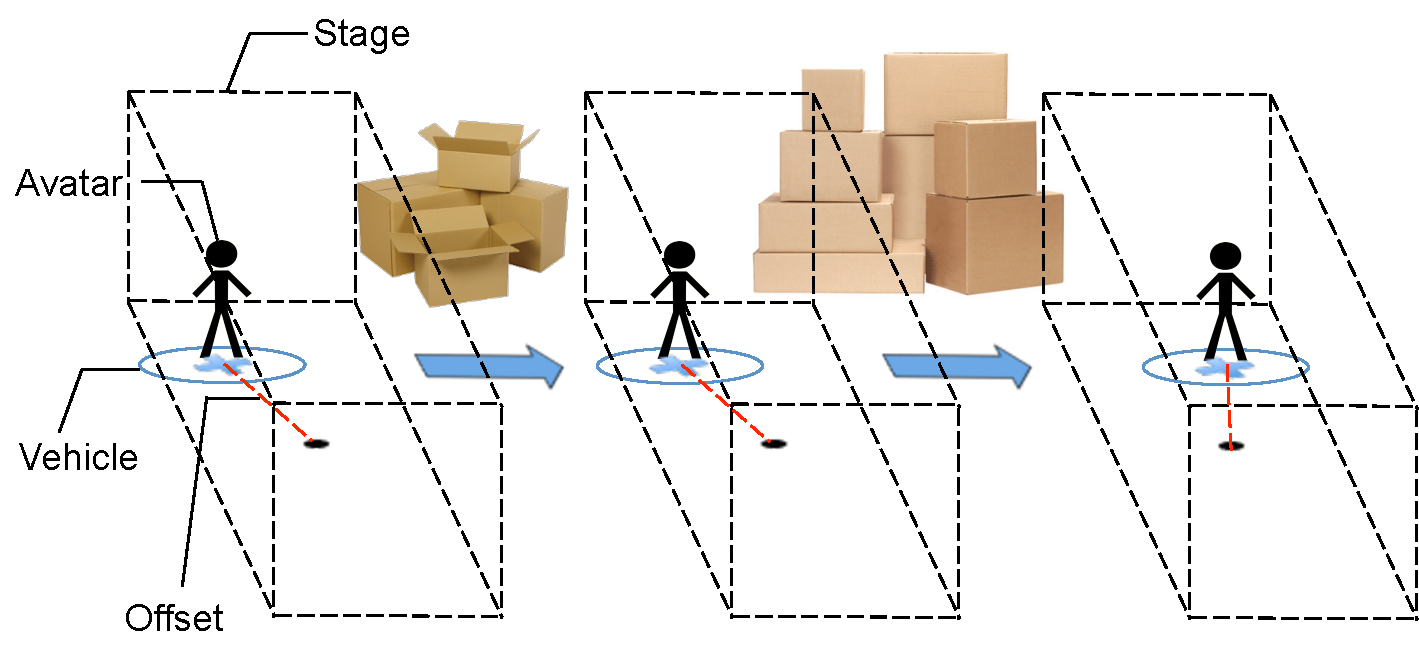
\includegraphics[width=.8\textwidth]{figures/ch2/vehicle}
  \caption{\label{fig:2_vehicle}Illustration of virtual vehicle based navigation.}
\end{figure}

We name this reference frame as a vehicle instead of conveyor mainly for two reasons: first, rate control navigation techniques provide similar navigation experience as we drive or pilot vehicles in the real world; second, we can reproduce some ``realistic" vehicle-based navigation behaviors (e.g. collisions, frictions) by adding constrains to the virtual vehicle without physicalize the whole virtual scene.

As a summary, the virtual vehicle provides a standard abstraction which facilitates the design of rate control navigation techniques, we just need to concentrate on how to control the vehicle. This conceptual model also makes it easier to understand user's velocity perception within immersive displays. When the user can move in the physical workspace, the navigation velocity perceived by the user is the sum of the virtual vehicle's velocity and user's velocity in the real workspace: 

\begin{equation}
\overrightarrow{v_{perceived}} = \overrightarrow{v_{vehicle}} + \overrightarrow{v_{user}}
\end{equation}


\subsection{Navigation in Multi-user IVE}
In a multi-user immersive virtual environment, existing studies on co-located collaboration focused mainly on closely-coupled collaboration (e.g. co-manipulation) in consistent mode. In this situation, virtual navigation is often disabled. When users need to change the place for collaboration, navigation is conducted in a leader-follower mode that one user controls the navigation for the whole group. Spatial consistency is always maintained \citep{Beck2013IGG} (Figure~\ref{fig:2_group_navig:group_navig_1}) or temporarily disabled \citep{Kulik2011CSS} in certain cases to avoid virtual obstacles (Figure~\ref{fig:2_group_navig:group_navig_2}).

\begin{figure}[htb]
  \begin{subfigure}{.5\textwidth}
    \centering
    \includegraphics[height=5cm]{figures/ch2/group_navig_1}
    \caption{Group navigation controlled by the user on the left using a trackball.}
    \label{fig:2_group_navig:group_navig_1}
  \end{subfigure}
  \begin{subfigure}{.5\textwidth}
    \centering
    \includegraphics[height=5cm]{figures/ch2/group_navig_2}
    \caption{Users' viewing frustums are shifted towards the open passage to avoid passing through the wall.}
    \label{fig:2_group_navig:group_navig_2}
  \end{subfigure}
  \caption{\label{fig:2_group_navig}Navigation of co-located users controlled by a leader.}
\end{figure}

The virtual vehicle along with the IIVC model can be easily adapted to manage multiple co-located users in immersive virtual environments. Each user has his/her own copy of stage and virtual vehicle (Figure~\ref{fig:2_multi_vehicle}) which allows individual navigation. Group navigation can also be achieved by merging all the stages and giving the control of all vehicles to a leader. 

\begin{figure}[htb]
  \centering
  \includegraphics[width=.8\textwidth]{figures/ch2/multi_vehicle}
  \caption{\label{fig:2_multi_vehicle}Illustration of virtual vehicle based navigation.}
\end{figure}

In individual mode, individual navigation can be achieved by providing independent navigation metaphors for each user which gives users full control on their own virtual locations. However, using navigation metaphors based on users' physical movements may be problematic as users share the same physical workspace. Thus multi-user navigation models with individual navigation control should comply with user cohabitation constrains that will be discussed in the following section.


% -------------------------------------------------------------------------------------------------

\section{Addressed Issues}
As presented above, co-located collaboration in IVE contains two different collaborative modes: the consistent mode and individual mode. In consistent mode, users have a distribution of virtual spaces that are coherent with their physical workspace, which offers a similar interaction experience as in real world. On the contrary, users in individual mode have independent viewpoints which broadens supported collaborative scenarios with more flexible viewpoint control.

However, due to the inconsistency between users' spatial distributions in the virtual world and real workspace, the individual mode provides users with a new kind of perceptual immersion and related cognitive experiences as they need to handle information from both real world and the virtual scene at the same time. We identified two main categories of spatial issues: perceptual conflicts during user communication and interaction, and user cohabitation in limited physical workspace. These issues should be studied if we want to validate the use of individual mode for co-located collaboration in IVEs. 


\subsection{Perceptual Conflicts}
Communications between collaborators are usually conducted in a multimodal way \citep{Paggio2005Multimodal} including verbal and non-verbal modalities \citep{Ennis2010Seeing, Dodds2011Talk}, especially deictic gestures to refer to objects or places. In individual mode, this kind of spatial interactions can be restored by introducing embodied avatars just like in remote situations - each user interacts temporally with other users' avatars instead of the real user in his/her own ``copy" of virtual world.  As a consequence, multimodal interactions in individual mode lead to two kinds of perceptual conflicts:

First, in projection-based immersive systems, users sharing the same display may sometimes enter each other's field of view when they work with embodied avatars. The simultaneous perception of a user and his/her avatar leads to a special experience that we called ``dual-presence". The dual-presence offers conflicting visual cues because the perceived real user and corresponding avatar share some common properties in terms of appearance and body movement (animated by real-time motion capture).

For example, in a two-user collaborative scenario (Figure~\ref{fig:2_pc_dualpresence}), user A is pointing at a cube next to him/her for user B to delete it. User B may be troubled by seeing both the real user A and his/her avatar doing the pointing gesture, and it may be more confusing when there happens to be another virtual object (e.g. a cylinder) in the pointing direction of real user A.

\begin{figure}[htb]
  \centering
  \includegraphics[width=.7\textwidth]{figures/ch2/pc_dualpresence}
  \caption{\label{fig:2_pc_dualpresence}Illustration of dual presence with a two-user scenario, two users are virtually face-to-face while standing side-by-side. User B simultaneously perceives that the real user A and A's avatar is pointing at different virtual objects.}
\end{figure}

Second, in individual mode, users dialogue with each other while interacting via embodied avatars. Since co-located users talk to each other directly without computer mediation, hearing someone from a different location than his/her visual representation (i.e. avatar) results in a visual-auditive conflict. Still in a two-user example (Figure~\ref{fig:2_pc_visualauditive}), user B is looking at user A's avatar in front, but the audio source (i.e. real user A) is on his/her left.

\begin{figure}[htb]
  \centering
  \includegraphics[width=.7\textwidth]{figures/ch2/pc_visualauditive}
  \caption{\label{fig:2_pc_visualauditive}Illustration of visual-auditive conflicts with a two-user scenario. User B experiences visual-auditive spatial conflicts when focusing on user A's avatar in front while talking to the real user A situated at a different location.}
\end{figure}

Although according to \citet{Spence2013Just}'s review, spatial coincidence does not represent a general constraint on multi-sensory integration in humans, but would be a much more task-dependent phenomenon. However, in a multi-user IVE, this visual-auditive conflict could be amplified due to the flexibility of virtual environment. For example, users could be far away from each other in the virtual world and they still hear each other from a close distance.

These two categories of perceptual conflicts are interrelated since they all depend on the distance between a user and his/her avatar. We need to study the usability of individual mode for co-located collaboration by investigating users' reaction to dual-presence and visual-auditive conflicts. The effects of such perceptual conflicts will influence choices on the design of co-located collaborative immersive systems. For example, whether we should prevent users from seeing the real users to avoid dual-presence, whether we need headphones to map users' speech to avatars' positions by 3D audio, etc.


\subsection{User Cohabitation}
Users in a multi-user IVE are subjected to two kinds of spatial constrains: users are inside a limited physical workspace, and they share the same workspace. These two constrains lead to different aspects of user cohabitation management: how to manage the spatial relationship between active users and the workspace boundaries while keeping good visual immersion? How to allocate personal workspace for users so that they won't collide or occlude each other?

Immersive virtual environment has the power to bring users to an artificial world by blocking the perception of the real world. In such situation users often forget boundaries of the physical workspace due to visual immersion, so when they move around in such system they risk to run into walls (with HMDs) or screens (projection-based display) which could endanger both the user and the device. Moreover, visual immersion is limited by functional tracking area and the screen configuration (for projection-based display). For example, in large projection-based immersive systems with non-closed displays such as large image wall or a 3-wall CAVE, visual immersion is limited to the display area (Figure~\ref{fig:2_illu_system}).

\begin{figure}[htb]
  \centering
  \includegraphics[width=0.49\textwidth]{figures/ch2/illu_wall_col}
  \includegraphics[width=0.49\textwidth]{figures/ch2/illu_empty}
  \caption{\label{fig:2_illu_system}Illustration of workspace boundary for translation (left) and looking direction (right) in a multi-stereoscopic 3-wall CAVE.}
\end{figure}

\begin{figure}[htb]
  \centering
  \includegraphics[width=0.49\textwidth]{figures/ch2/illu_user_col}
  \includegraphics[width=0.49\textwidth]{figures/ch2/illu_occ}
  \caption{\label{fig:2_illu_users}Illustration of collision (left) and occlusion (right) between co-located users in a multi-stereoscopic 3-wall CAVE.}
\end{figure}

When multiple users share the same immersive device for co-located collaboration in individual mode, they may run into collision when they move around without paying attention to the others. In projection-based immersive systems, one's visual perception of the virtual world could be disrupted by another if the latter appears to be in the field of view of that user due to body occlusion (Figure~\ref{fig:2_illu_users}).

Depending on the choice of display technology and screen configuration, not all aforementioned issues are present in all types of immersive systems. Here Table~\ref{tab:cohab_issues} divides all cohabitation issues into different categories: some are inherent issues of the individual collaborative mode, others are more system-dependent, i.e. depending on the type and configuration of used immersive display. For example, user occlusion merely appears in projection-based immersive system, and perceiving ``empty screen" is only possible with non-closed immersive display. 

\begin{table}[htb]
\renewcommand{\arraystretch}{1.3}
\caption{Cohabitation Issues in Multi-user Immersive Systems.}
\label{tab:cohab_issues}
\centering
\begin{tabular}{l l l}
  \hline
   & Workspace-related & User-related \\ \hline
  Generic & Collision with workspace border & Collision between users \\
  System-dependent & Seeing non-projected area & User occlusion \\ \hline
\end{tabular}
\end{table}

For safe and efficient use of multi-user IVEs, new paradigms are needed to enable individual navigation in infinite virtual space while keeping users' level of immersion and safety.

% -------------------------------------------------------------------------------------------------

\section{Approach}
To assess users' reactions to certain stimuli (e.g. perceptual conflicts) or the performance of novel paradigms (e.g. paradigms for navigation or object manipulation) in virtual environments, experiment-based user evaluation inherited from HCI research has become a mainstream method. Besides formative user experiment, there are many other evaluation methods such as cognitive walkthrough, heuristic expert evaluation, interview, post-hoc questionnaire and so on, each can help us to gather some information from a different angle with certain cost \citep{Bowman2002Survey}.

In the context of this thesis, our goal is to study spatial issues related to individual collaborative mode in order to design a valid and efficient framework for co-located collaboration in IVE. All experiments discussed below are conducted in projection-based immersive system in which all spatial issues that we mentioned are present. The main experimental platform named EVE (Evolutive Virtual Environment), is a four-screen multi-user immersive CAVE system built with the active \& passive separation technique (see Appendix~\ref{appendix:platform}). It serves as an experimental tool to study issues related to user interaction and communication for co-located collaboration in projection-based multi-user immersive virtual environment.

The first step is to study effects and influencing factors of perceptual conflicts due to the introduced avatar representation for co-located collaboration. We want to examine how perceptual conflicts generated by dual-presence would alter users' communication and their task performance. In a two-user case study, participants receive instructions from an experimenter to accomplish an object-picking task, we artificially created different levels of perceptual conflicts by varying the distance between the real experimenter and her avatar, and also by changing modalities involved in the instructions (verbal and/or gestural). A post-hoc questionnaire was designed to collect users' subjective feelings towards dual-presence and their understanding of the instructions. This experiment is presented in detail in Chapter~\ref{chapter:expe_perception}.

Second, we concentrate on the design and evaluation of appropriate navigation paradigms to allow individual navigation while solving user cohabitation problems in a progressive way. The paradigm that we propose is based on a Human Joystick metaphor controlled by head tracking \citep{Bourdot2002HCNav}. First we evaluated this metaphor by a comparative experiment \citep{Chen2013NVW} to confirm its advantages over traditional navigation solutions (e.g. joystick). Then we created an Altered Human Joystick paradigm by adding additional controls to manage users' relationship with system borders and to minimize inter-user interferences.

At last, by taking into account feedbacks of existing studies, we continue to make improvements on the human joystick paradigm in the aim of providing a generic framework for co-located collaboration which integrates constrains from the physical workspace and virtual world into the navigation control as described in Chapter~\ref{chapter:dynamic_model}.

% -------------------------------------------------------------------------------------------------

\section{Conclusion}
The research described in this thesis consists of investigating how to enable individual mode to better support co-located collaboration in multi-user IVEs. The first part of this chapter outlines motivations and techniques to create immersive systems for co-located collaboration, and the second part presents notions around spatial organization of users' workspaces and how we navigate in IVEs. Then the last part summarizes issues related to spatial aspects of co-located use of IVE, it also presents research efforts that we made to study these issues and to propose solutions accordingly.

In following chapters, we present separately our studies on perceptual and cohabitation issues that we identified in the aim of building a general framework for co-located collaboration in IVE which allows both consistent and individual modes.
\chapter{User Cohabitation for Individual Navigation Tasks in Restricted Physical Workspace}
\label{chapter:cohabitation}

\section{Taxonomy}

Navigation is one of the most important and fundamental interaction that we have within the virtual environment.

A lot of navigation techniques of different nature exist to allow users to travel through large virtual space, while physically stay within a limited workspace. These navigation techniques can be classified according to the control law - how a given input from the user can be mapped to a position or velocity change in the virtual world. Typical control laws include position and rate control, and can be implemented by both hardware and software solutions.

The most studied position control is natural walking, which is considered to be the most intuitive way to explore the virtual environment \citep{Ruddle2009BW}. To enable infinite walking in restricted real workspace, one can use both physical locomotion devices like treadmills \citep{Iwata1999Treadmill} and software solutions (e.g. redirection \citep{Peck2008RED}, resetting \citep{Williams2007ELV} and scaling techniques \cite{Interrante2007SLB}). Besides natural walking, walk-in-place \citep{Razzaque2002RWP} and WIM (World-In-Miniature) \citep{Stoakley1995VRW} are also interesting alternatives. Moreover, \citet{Fleury2010Generic} proposed a general model to integrate physical workspace into the virtual world and make the user aware of the physical environment in different ways. \citet{Cirio2012Cube} also summarized several metaphors for safe navigation in a restricted cubic workspace.

Conversely to previous techniques, rate control techniques are based on a virtual vehicle model which enables navigation in large virtual scenes. Users control directly the vehicle's velocity instead of position in the virtual world and can have the sensation of moving (self-motion illusion or vection \citep{Riecke2012Vection}). Actually the virtual vehicle can be controlled by information coming from different sources, for example, various input devices like joystick, haptic arm \citep{Martin2012HDF} or even specific locomotion devices \citep{Marchal2011JOYMAN}. With video cameras or optical tracking systems, users can specify the velocity of the vehicle by motion tracking data of the hand (camera-in-hand \citep{Ware1990EVC}) or head movements \citep{Bourdot2002HCNav}. Gestures \citep{Konrad2003GesturePlay} and postures \citep{Kapri2011Steering} can also be used to move the virtual vehicle. Bowman et al. named this kind of virtual navigation techniques steering metaphors \citep{Bowman2004UIT} which are often relatively easy to implement and can provide efficient and flexible control of virtual navigation.

Some navigation metaphors such as the bubble technique \citep{Dominjon2005Bubble} and the magic barrier tape \citep{Cirio2009MBT} combine both position and rate control in order to enable infinite navigation within restricted real workspace. Position control is used within the physical workspace and then rate control is applied to the virtual vehicle to move further in the virtual world.

\section{6DoF Head Controlled Navigation}

\section{Evaluation}

It's not obvious to compare different navigation techniques without a given virtual context and the associated task. Nevertheless, \citet{Bowman1997TIV} have proposed a list of quality factors which can help us to compare and measure the performance of navigation techniques including general performance indicators such as velocity and accuracy, spatial awareness, ease of learning, ease of use, and level of presence. General performance indicators are relatively easy to measure. We can choose factors that we need depending on the given task and the configuration of the virtual scene.

The level of presence is an important factor for the use of navigation techniques in an immersive virtual environment. \citet{Slater1994DepthPre} consider presence as a subjective phenomenon that can be defined as the sensation of being in a virtual environment, while \citet{Witmer1998MPV} relate presence in part to the concept of attention. These authors believe that both involvement and immersion are necessary for experiencing presence. \citet{Schuemie2001Pres} have proposed a taxonomy of different measures of presence and a detailed analysis of factors that influence presence in the virtual environment.

Another important factor is the user comfort, particularly the lack of symptoms related to cybersickness. \citet{Rich1996AICS} have examined the relationship between the user's level of control of his/her own movements and cybersickness, while \citet{So2001ENS} have carried out experiments to study the influence of the navigation speed (both linear and circular components) on the level of severity of cybersickness. A study by \citet{Stanney2002HPIVE} gives us a better global view that addresses different perceptive factors that are susceptible to cause cybersickness. \citet{LaViola2000DCV} has also discussed about the physiological aspects and theories of cybersickness. To evaluate the level of cybersickness, the Simulator Sickness Questionnaire (SSQ) \citep{Kennedy1993SSQ} remains the reference tool despite the development of various physiological measurements.

\section{Cohabitation}

When it comes to managing multiple users in the same immersive virtual environment for co-located collaboration, most works focused on closely coupled stage situations. In this case, either virtual navigation is disabled (they can just walk inside the tracking area for observation or co-manipulation), or their navigation is controlled by a leader and shared by other users~\citep{Beck2013GGT, Kulik2011CSS}. To enable more complex collaborative scenario including both loosely coupled and closely coupled tasks, it is interesting to allow safe individual navigation for co-located users.
\chapter{Study on User Cohabitation}
\label{chapter:user_cohab}
\pagebreak

\textbf{Chapter Abstract}

This chapter .

\vspace*{2\baselineskip}

\minitoc

\newpage
\section{Introduction}
To support safe and functional individual navigation in an multi-user IVE, traditional navigation metaphors should be adapted according to the number of co-located users and the configuration of the immersive system (size and shape of the screen walls, effective tracking space, etc.) to avoid cohabitation problems that we summarized in Chapter~\ref{chapter:colocated_colab}.

This chapter consists of two sections. The first summarizes conceptual details about a navigation paradigm we designed called Altered Human Joystick metaphor. The idea of this metaphor is to let each user navigate with normal human joystick control and the system will introduce alterations to a user's navigation velocity according to his/her spatial relationship with other users and with respect to the physical workspace, in order to keep user's safety and immersion level.

The second presents several user experiments that we conducted to verify the effectiveness of cohabitation control and their impacts on users' navigation performance and subjective feelings. First, we tested several alterations accumulatively in a collaborative case study, then three refined experiments followed to give an exhaustive analysis of different combinations of these alterations respectively in translation-only, rotation-only and translation-rotation combined navigation conditions.


\section{Approach - Altered Human Joystick}
In an immersive virtual environment, the human joystick paradigm allows virtual navigation by physical movements relative to a fixed reference frame. It can not assure safe and efficient navigation because it does not take into account the spatial limitations of the physical system. Users need to make sure themselves to stay inside a safe zone without touching any physical obstacles and to stay within usable projection areas. So we proposed some alterations of the original paradigm to free user's mind from these constrains.

\subsection{Basic Model}
The basic navigation method that we use is a reduced version (from 6DoF to 3DoF) of a head-controlled navigation technique (Figure~\ref{fig:4_hcnav}) proposed by \citet{Bourdot2002HCNav}. It is actually a human joystick metaphor \citep{McMahan2012EDF}, but with an additional degree of freedom for yaw rotation. User's head position and orientation are captured in real time with an optical tracker attached to the 3D glasses. With Human Joystick metaphor users' hands can be left over for object manipulation or gesture interaction. This ratio control technique requires a user to move physically and thus involves his/her vestibular system during navigation, which could potentially reduce symptoms of cybersickness \citep{Chen2013NVW}.

To navigate, user first needs to choose a neutral reference frame (composed of a position and an orientation ($P_{0}, \theta_{0}$)) during calibration. Then user can move in the real workspace relatively to this reference frame to control the linear and angular velocity of the vehicle ($\overrightarrow{v_{veh}}, \Omega_{veh}$), denoting $(P, \theta)$ the current configuration. The translation and rotation transfer functions are configured respectively by coefficients $K_{T}$ and $K_{R}$.

\begin{equation}
\overrightarrow{v_{veh}}=K_{T}\cdot \overrightarrow{P_{0}P}
\end{equation}
\begin{equation}
\overrightarrow{\Omega_{veh}}=K_{R}\cdot \widehat{\theta_{0}\theta}
\end{equation}

\begin{figure}[tb]
  \centering
  \includegraphics[width=0.8\textwidth]{figures/ch4/HCNav}
  \caption{\label{fig:4_hcnav}Head-controlled navigation paradigm.}
\end{figure}

\subsection{Alterations}

\subsubsection{Altered Transfer Function}
\label{sec:altered_tf}
Rate control navigation metaphors are mainly characterized by their transfer functions. A transfer function transforms user's input into a change of the virtual vehicle's velocity. To restrain user's translational workspace, we can replace the linear transfer function with a divergent one integrating the distance limitation into the navigation model.

\begin{equation}
\overrightarrow{v_{veh}}=K_{T}\cdot \left(\frac{\Delta x}{X_{m}-\Delta x},\:\frac{\Delta y}{X_{m}-\Delta y}\right)
\end{equation}

where $X_{m}$ is the minimum distance from the neutral position $P_{0}$ to the border of the physical system (Figure~\ref{fig:4_workspace_border}a). This divergent transfer function allows user to apply an infinite vehicle velocity when reaching $X_{m}$. So the workspace of a user is defined by the physical space that user is free to move inside before reaching any borders.

\begin{figure}[htb]
\begin{center}
\includegraphics[width=0.8\textwidth]{figures/ch4/workspace_border}
\par\end{center}
\caption{\label{fig:4_workspace_border}a) The maximum available workspace $X_{m}$ can have different values on x and y axis. b) User's rotational workspace is defined by $\theta_{max}$ on both sides of the neutral orientation.}
\end{figure}

To avoid collision between users, we can consider each user as a moving border which restricts directly the workspace of other users. However, this method makes the velocity control too unstable when all users move the same time. A possible compromised solution is to assign each user a safe zone for proper use, and an overlapped zone to share with others. We adjust the ``virtual border" of one user's workspace depending on the penetration of other users in the shared area. This way a user's velocity will only be influenced by others when he/she is inside the shared zone, one can make use of the entire shared zone as if he/she was alone in the system until the other user also needs to use it. Figure~\ref{fig:4_adaptive_trans_border} shows an example of two users inside a 3-wall CAVE system. Usually CAVE-like systems are in a rectangular form, so the border formed by a user is chosen to be a vertical plane.

\begin{figure}[htb]
\begin{center}
\includegraphics[width=0.7\textwidth]{figures/ch4/adaptive_trans_border}
\end{center}
\caption{\label{fig:4_adaptive_trans_border}Adaptive border of user's workspace for translation in a two-user case : a) Initial state. b) User B moves into the shared zone while user A is still in the safe zone, both users' workspaces are not influenced and user B can use the entire shared zone. c) User A also moves into the shared zone and pushes the border of user B's workspace to the right. d) User B moves back to the safe zone, the entire shared zone can now be used by user A.}
\end{figure}

Considering rotations, physical constrains could also be integrated into the transfer function similarly as for translation. For example, in a 3-wall CAVE it is preferable to avoid user occlusions and prevent users from seeing the empty screen behind them. However, due to the different nature between translation and rotation movements, we chose to use a saturated quadratic transfer function rather than a divergent form as follows:

\begin{equation}
\Omega_{veh}=
  \begin{cases}
    \frac{\Omega_{max}}{(\theta_{max})^{2}}\cdot(|\Delta\theta|)^{2} & \text{if } |\Delta\theta|<\theta_{max} \\
    \Omega_{max} & \text{if } |\Delta\theta| \geq \theta_{max}
  \end{cases}
\end{equation}

where $\theta_{max}$ represents the maximum available rotational workspace (with which the user reaches the maximum rotation speed $\Omega_{max}=\pi\, rad.s^{-1}$) computed as the minimum of $\theta_{left}$, $\theta_{right}$ and $\theta_{user}$ to provide a symmetric vehicle control around the neutral orientation $\theta_{0}$ (Figure~\ref{fig:4_workspace_border}b).  


\subsubsection{Adaptive Neutral Reference Frame}

The original human joystick metaphor has a fixed neutral reference frame (a neutral position and orientation) defined during calibration. This reference frame should give user the maximum workspace that the physical working environment can offer, for example, the center of a CAVE is often a good choice. However, when we have mobile obstacles in the physical working environment, e.g. multiple co-located users, it may be inappropriate to have a fixed reference frame. With the above methods of computing user's available workspace, a fixed neutral reference frame distribution will often lead to non-symmetric use of the total available workspace both for translation and rotation.

To optimize workspace usage, we can reconfigure each user's neutral reference frame as the center of his/her available workspace (Figure~\ref{fig:4_neutral_ref}). In this way, each user's workspace is balanced between constrains introduced by the display system and by other users, and is always symmetric on the left and right with respect to the neutral reference frame.

Although this method could make better use of the total workspace, it also potentially increases the mutual influence between users, which may be disturbing for the navigation control. When users have relatively small workspace, the variation of neutral reference frame may remain imperceptible during navigation, which is to be tested.   

\begin{figure}[htb]
  \centering
  \includegraphics[width=0.7\textwidth]{figures/ch4/neutral_ref}
  \caption{\label{fig:4_neutral_ref}(a, c) Users' neutral reference frames are fixed to the initial distribution. (b, d) Users' neutral reference frames are computed dynamically according to both users' positions.}
\end{figure}

\subsection{Combinations}
With the two categories of alterations presented above, we can create a set of similar navigation methods by combining these modifications. To see more clearly the impacts of each modification, we created three groups of navigation methods (see table~\ref{tab:4_combinations}). In the first two groups (Group T and Group R), we deactivated respectively rotation and translation, and we kept both for the last group (Group TR). For Group R, since users are not supposed to change their positions, the neutral orientations will always be fixed, though they will be different depending on how they are computed (be facing the front screen or be the bissectrice of rotational workspace).

\begin{table}[hbt]
\renewcommand{\arraystretch}{1.3}
\caption{A List of Altered Versions of Human Joystick divided in Three Groups (``/" means undefined)}
\label{tab:4_combinations}
\centering
\begin{tabular}{c l l l l}
  \hline
  Technique & \multicolumn{2}{c}{Translation} & \multicolumn{2}{c}{Rotation} \\
   & Form & Neutral Position & Form & Neutral Orientation \\ \hline
  T1 & Linear & Fixed & / & / \\
  T2 & Linear & Adaptive & / & / \\
  T3 & Divergent & Fixed & / & / \\
  T4 & Divergent & Adaptive & / & / \\ \hline
  R1 & / & / & Linear & Face front screen \\
  R2 & / & / & Linear & Bissectrice \\
  R3 & / & / & Saturated Quadratic & Face front screen \\
  R4 & / & / & Saturated Quadratic & Bissectrice \\ \hline
  TR1 & Linear & Fixed & Linear & Fixed \\ TR2 & Linear & Fixed & Linear & Adaptive \\
  TR3 & Linear & Adaptive & Linear & Fixed \\ TR4 & Linear & Adaptive & Linear & Adaptive \\
  TR5 & Divergent & Fixed & Saturated Quadratic & Fixed \\ TR6 & Divergent & Fixed & Saturated Quadratic & Adaptive \\
  TR7 & Divergent & Adaptive & Saturated Quadratic & Fixed \\ TR8 & Divergent & Adaptive & Saturated Quadratic & Adaptive \\
  \hline
\end{tabular}
\end{table}


% -------------------------------------------------------------------------------------------------


\section{Evaluation Framework}
To evaluate the contributions of alterations described above, we defined several categories of metrics. Then we used them to compare these altered human joystick models by doing different navigation tasks within our CAVE platform.

\subsection{Measures}
We are interested in information coming from two different sources: how well users could achieve goals and manage navigation in the virtual world, and how they position themselves with respect to the screens and other users in the physical workspace. Here we summarized three categories of measurements that we used for evaluation.

\subsubsection{Navigation Performance Metrics}
For a pure navigation task, measurements like task finishing time (or speed) and trajectory length are often used to evaluate user's navigation efficiency.

\subsubsection{User Cohabitation Capacity Metrics}
User cohabitation concerns both users' spatial relationship with the limitation of physical system and disturbance between users. We propose an evaluation model containing four variables covering all these aspects to measure user cohabitation capacity in a restricted physical workspace.

When several autonomous entities move within a restricted physical workspace, whether they will have cohabitation problem depends not only on where they are, but also on the moment when they have spatial coincidence. So all these variables combine spatial and temporal dimensions, and higher scores suggest higher disturbance level.

\paragraph{Hazardous Area Consumption}
In the real world, we choose to define an ``Hazardous area" including all positions closer than $D_{Hazard}=1$ meter to any physical obstacle as shown on Figure \ref{fig:4_metrics}a.

In this area, user's presence and safety may be in balance depending both on the user real speed $\overrightarrow{v_{real}}$ which may affect collision probability, and on his/her relative distance to the screens $d_{screen[i]}$. So we compute a relative score $V_{hac}$ based on $\overrightarrow{v_{real}}$ and $d_{screen[i]}$ when the user is inside the hazardous area. 

\begin{equation}
S = 
  \begin{cases}
  \overrightarrow{v_{real}}\cdot\overrightarrow{n_{i}} & \text{if } \overrightarrow{v_{real}}\cdot\overrightarrow{n_{i}} \leq 0 \\
  0 & \text{if } \overrightarrow{v_{real}}\cdot\overrightarrow{n_{i}} > 0
  \end{cases}
\end{equation}

\begin{equation}
V_{hac}=\sum_{t_{initial}}^{t_{final}}\left(\sum_{i=1}^{i=3}\left(\frac{S}{d_{screen[i]}}\right)\right)
\end{equation}
where $\overrightarrow{n_{i}}$ is the screen's normal vector.


\paragraph{Shared Workspace Occupation}
In a two-user case, they share part of their translation workspace. To estimate the probability of user collision in the shared zone, we measure each user's penetration distance in the shared workspace $\Delta P_{sh}(t)=\left|(\overrightarrow{P}-\overrightarrow{P_{0}}).\overrightarrow{x}\right|$ while the other user is also inside the shared area (cf. Figure \ref{fig:4_metrics}b), and $\Delta P_{sh}(t)=0$ otherwise.

\begin{figure}[tb]
  \centering
  \includegraphics[width=0.7\textwidth]{figures/ch4/cohab_metrics}
  \caption{\label{fig:4_metrics}(a) The hazardous area. (b) User's penetration $\Delta P_{sh}(t)$ in the shared zone. (c) Illustration of seeing empty screen angle $\theta_{emp}(t)$ and (d) the occlusion angle $\theta_{occ}(t)$.}
\end{figure}

Using this penetration information, we can define a variable $V_{Psh}$ allowing to evaluate users' shared area usage taking in account both amplitude and duration of each user's usage situation as:

\begin{equation}
V_{Psh}=\int_{t_{init}}^{t_{final}}\Delta P_{sh}(t)\cdot dt
\end{equation}

\paragraph{Empty Screen Perception}
We define a variable $V_{emp}$ to evaluate to what extent and how long a user sees the empty screen behind by using $\theta_{emp}(t)$ (Figure \ref{fig:4_metrics}c)

\begin{equation}
V_{emp}=\int_{t_{init}}^{t_{final}}\theta_{emp}(t)\cdot dt
\end{equation}

\paragraph{User Occlusion}
In order to evaluate the occlusion phenomenon, we define a penalty angle $\theta_{occ}(t)$ which quantifies the non-usable part of the field of view where the perception of other users disrupts the perception of the virtual world as shown on Figure \ref{fig:4_metrics}d. This angle can be expressed, using the current user position $P$, the head orientation $\overrightarrow{H}$, the total available field of view $\theta_{fov}$ , the other user position $P'$ and a bounding cylinder radius $R$ which represented the size of the disturbing user, as:

\begin{equation}
\theta_{occ}=\frac{\theta_{fov}}{2}-\widehat{(\overrightarrow{H,}\overrightarrow{PP'})}+arcsin(\frac{R}{\left\Vert \overrightarrow{PP'}\right\Vert })\mathrm{\:,\: with\:}\theta_{occ}\geq0
\end{equation}

Using this occlusion angle, we define a variable $V_{occ}$ which allows to evaluate the importance of the occlusion problem considering both occlusion amplitude and duration computed as:

\begin{equation}
V_{occ}=\int_{t_{init}}^{t_{final}}\theta_{occ}(t)\cdot dt
\end{equation}


\subsubsection{Subjective Questionnaires}
Questionnaires are very useful tools to get user's subjective feelings (like presence and cybersickness) and explanations of certain choices and behaviors.

In our experiments, since we compared similar navigation conditions with minor differences, the level of presence was not our primary concern. However, these alterations could be source of cybersickness, so we used the Simulator Sickness Questionnaire (SSQ) \citep{Kennedy1993SSQ} to assess user's level of cybersickness before and after each test. In addition, we developed a light-weight cohabitation questionnaire to further investigate user's feeling towards disturbances coming from physical surroundings as well as from the other user (see Appendix~\ref{appendix:cohab_q}).


\subsection{Pre-test Condition}
In all the experiments below we tested the cohabitation of two users. The initial distribution of both users' neutral reference frames was defined as follows: each user's neutral position had equal distance to the nearest obstacle on the left and right, and they were moved 0.6m away from the front screen to leave more space for user to move forward. The neutral orientations were chosen to be face the front screen (Figure~\ref{fig:4_initial_config}). At the beginning of each task trial, users were always situated at the neutral position and facing the neutral orientation.

\begin{figure}[htb]
  \centering
  \includegraphics[width=0.8\textwidth]{figures/ch4/initial_config}
  \caption{\label{fig:4_initial_config}The initial distribution of users' neutral reference frames in our CAVE platform.}
\end{figure}

Before passing real tests, participants joined a training session during which they spent about three to five minutes in a virtual playground to get familiar with the original human joystick metaphor.


% -------------------------------------------------------------------------------------------------


\section{Collaborative Case Study}
\subsection{Experimental Design}
We conducted a first user study \citep{Chen2015Cohab} with 36 participants divided into pairs to test modified transfer functions in a two-user working scenario. We defined three test conditions:

\begin{itemize}
  \item \textbf{C1}: Original human joystick with linear transfer functions for translation and rotation (served as control condition).
  \item \textbf{C2}: Human joystick technique with modified transfer functions.
  \item \textbf{C3}: C2 plus adaptive neutral orientation.
\end{itemize}

Back then, the idea of adaptive neutral reference frame was not fully developed and we were not sure whether that would be beneficial, so we formed C3 in addition to C2 as a beta test of reorientation of the neutral reference frames (their positions remained fixed).

We assumed that modified transfer functions (C2) would improve users' cohabitation capacity, thus improve their navigation performance compared to linear transfer functions (C1). We also assumed that as adaptive neutral orientation provided better distribution of user's rotational workspace, users should have less occlusion with C3 than C2.

Participants were invited to accomplish an object-finding task inside a virtual factory (Figure~\ref{fig:4_teaser_exp1}). The factory had five similar sections each containing a common working zone and two storage areas connected by corridors. The task was for each participant to bring target objects from different storage areas to the common working zone. Since the task was relatively complicated (based on a realistic working scenario) and had a pre and post questionnaire session (for the evaluation of cybersickness), we used a between-subject design with each pair of participants testing one of the three conditions.

\begin{figure}[htb]
  \centering
  \includegraphics[width=0.8\textwidth]{figures/ch4/teaser_exp1}
  \caption{\label{fig:4_teaser_exp1}Two users worked inside a multi-stereoscopic CAVE system to finish an object-finding task. They were virtually face to face to put down collected objects.}
\end{figure}

\subsection{Results}
To summarize, participants had similar navigation performance both in terms of speed and precision under different conditions. And for user cohabitation capacity, main effects were found on Shared Workspace Occupation ($V_{Psh}$) (H(2, N=36) = 6.109610, p=0.047) with C3 (mean=1.402, sd=0.921) less than C2 (mean=2.826, sd=1.431), and on Occlusion Angle ($V_{occ}$) (H(2, N=36) = 21.08269, p\textless{} 0.0001) with C3 (mean=14.7, sd=31.0) less than C1 (mean=153.4, sd=71.4) and C2 (mean=90.3, sd=84.9).

Participants under all three conditions experienced mild cybersickness symptoms (Total score: C1: mean=15.58, sd=20.41; C2: mean=18.39, sd=19.37; C3: mean=13.4, sd=10.51), however, no significant difference were found between these conditions.

\subsection{Discussion}
The lack of significant difference between C1 and C2 could be explained by several observations. First, during navigation tasks, users were not necessarily synchronized with each other and were free to choose their navigation speed and trajectory. Regarding navigation control, they also had the choice between yaw rotation and lateral displacements, combined with forward movement to achieve the same virtual trajectory. Therefore it was difficult to predict users' real world movements and the recorded data had a large subject-dependent variation. Second, users were generally more cautious and conservative than we expected. They rarely went too close to the screen or to the other user to get high navigation speed by fear of running through virtual walls or barrels, which lessened cohabitation problems. The average navigation velocity measured under the three conditions were similar (around 2 m/s), which meant that the divergent part of C2 and C3 were seldom reached by users with the given gain values.

Finally, C3 was proved to have better support for reducing user occlusion. The way we defined the neutral orientations provided symmetric rotational workspace for users and tended to maintain an open angle between neutral orientations. In addition, we observed that C3 was also the best technique to minimize the occupation of the shared workspace (cf. $V_{Psh}$). Actually, as the neutral orientation defined user's main walking axis, the adaptive neutral orientations allowed more frequent use of safe zones rather than the shared zone in the middle.

Although we did not find significant results to prove the benefits of modified transfer functions as we assumed in this experiment, important lessons were learned for future study of user cohabitation in a multi-stereoscopic immersive system. First of all, for a given task inside an immersive device with fixed size, a properly chosen gain value can reduce the chance for having user cohabitation problems even with linear transfer function. In other words, to show the limitations of linear transfer functions, we should use smaller gain value. Second, it was difficult to distinguish the influence of each individual modification due to the divergence in users' navigation strategies. To tackle that, we could test translation and rotation under separate conditions (Group T and Group R) as presented in Table~\ref{tab:4_combinations}. At last, we found it beneficial to have adaptive neutral orientation, which led us to extend the alterations by setting the neutral position $P_{0}$ of each user dynamically to see if we can get similar benefits as performing neutral orientation change. So besides C1, C2 and C3, which corresponded respectively TR1, TR5 and TR6 (Table~\ref{tab:4_combinations}), we made a complete list of eight conditions to test all possible combinations.

Moreover, the alterations tested in this experiment did not seem to provoke more symptoms of cybersickness, which made it viable for us to extend the model and conduct more refined experiments.


% -------------------------------------------------------------------------------------------------


\section{Follow-up Experiments}
We conducted three additional experiments to complete previous user study. As explained above, we globally lowered the base gain value for all transfer functions. In Experiment T (Translation only) and Experiment R (Rotation only), we created two special groups of navigation conditions by cutting off respectively rotation and translation, while in Experiment TR (Translation with Rotation) we kept both. All the three groups of conditions were listed in table \ref{tab:4_combinations} and to be tested with different types of navigation tasks. 

We compared these conditions in terms of navigation performance and cohabitation capacity to see the influence of each alteration and the effect of their combinations. What's different from previous user study was that participants were equipped with closed headphones to avoid perceiving the other user by audio cues (foot steps, verbal communications, etc.) since the alterations of the navigation metaphor only provided visual feedback.

Based on the results of previous experiment, we did not measure the level of cybersickness this time because of the number and similarity of test conditions. Instead, we used a light-weight questionnaire in Experiment TR (Appendix~\ref{appendix:cohab_q}) to get additional information on user cohabitation.

For all the experiments below, we performed one-way ANOVA test to compare different variables as within-subject factors. For post-hoc analyses, we used TukeyHSD multiple comparisons of means. All the analyses were performed with R\footnote{http://www.r-project.org/}. The results presented in this section were considered statistically significant when p \textless{} 0.05. Results having a p value between 0.05 and 0.1 were also presented as a trend effect.

\subsection{Participants}
12 participants (11 male, 1 female), aged from 24 to 54 (mean=32) were involved in our user study. They were divided into six pairs and each pair passed successively Experiment T, R and TR.


\subsection{Experiment T}
\subsubsection{Experimental Design}
To compare the four navigation techniques in the first group (T1 - T4), we asked participants to accomplish a navigation task several times with each time a different technique. Thus, each navigation technique was tested once and the four conditions were randomized for different groups of participants.

The task was to travel to the other side of a straight corridor by following a given path marked by a white line on the floor and crossing all the gates along the path (Figure~\ref{fig:4_task1}). Each pair of participants had parallel corridors with symmetric path to walk through so they have more chance to collide in the physical workspace. To begin, participants left their departure areas and traveled to destination zones on the other side of the corridors. Once both participants arrived, they were teleported to the departure areas to begin the next round with a different navigation technique till all the conditions were tested.

\begin{figure}[htb]
  \centering
  \includegraphics[width=0.8\textwidth]{figures/ch4/t1}
  \caption{\label{fig:4_task1}A screen-shot of the virtual scene used in Experiment T.}
\end{figure}

\subsubsection{Results}
We first tested the effects on two independent variables: the translation transfer function (linear or divergent) and neutral position type (fixed or adaptive). Then to see interaction effects between these two variables, we further compared the four navigation techniques.

\begin{table}[hbt]
\renewcommand{\arraystretch}{1.3}
\caption{Results of Experiment T (Translation only), $\varnothing$ means non significant result.}
\label{tab:4_result_t1}
\centering
\small
\begin{tabular}{p{3cm} l l p{4.5cm}}
  \hline
  Variable & Transfer Function Type & Neutral Position Type & Technique T1 $\sim$ T4 \\
  \hline
  Time & Divergent\textless Linear & $\varnothing$ & T1\textgreater \{T3, T4\}; T2\textgreater T4 \\
  Length & $\varnothing$ & $\varnothing$ & $\varnothing$ \\
  Hazardous Area Consumption & Divergent\textless Linear & $\varnothing$ & T1\textgreater \{T3, T4\}; \\
  Shared Workspace Occupation & Divergent\textless Linear & $\varnothing$ & T1\textgreater T4; T1\textgreater T3 (0.054); T2\textgreater T4 (0.055) \\
  \hline
\end{tabular}
\end{table}

Results showed that the transfer function type had a significant influence on multiple dependent variables while the neutral position type did not (Table~\ref{tab:4_result_t1}). For navigation time, divergent transfer function (mean=89.5, sd=17.8) was faster than the linear one (mean=113.0, sd=21.1) (F(1, 46)=17.25, p\textless 0.001). For Hazardous Area Consumption, divergent transfer function (mean=111.57, sd=15.17) had lower score than the linear one (mean=132.58, sd=22.22) (F(1, 46)=14.63, p\textless 0.001). Same for Shared Workspace Occupation, divergent transfer function (mean=5.18, sd=3.26) had lower score than the linear one (mean=12.58, sd=8.99) (F(1, 46)=14.38, p\textless 0.001).


\subsection{Experiment R}
\subsubsection{Experimental Design}
We compared the four navigation techniques in the second group (R1 - R4) which only allowed rotations. We asked participants to turn each time virtually 180 degrees to perform an object picking task. Each navigation technique was tested once and the four conditions were randomized for different groups of participants.

The task was to pick up an object behind a user and put it into the orange cube on the table in front (Figure~\ref{fig:4_task2}). Participants were asked to stay on the neutral position and to keep their feet fixed on the floor since we did not want to involve translation. As a consequence, in this experiment we could only test a specific value of adaptive neutral orientation (the bissectrice of rotational workspace) compared to an empirically chosen direction (facing front screen).

We used green arrows to indicate the right rotation direction for the participants so overall they had equal left and right rotations.

\subsubsection{Results}
We first tested the effects on two independent variables: the rotation transfer function (linear or saturated quadratic) and neutral orientation type (face front screen or bissectrice). Then to see interaction effects between these two variables, we further compared the four navigation techniques.

\begin{figure}[htb]
  \centering
  \includegraphics[width=0.8\textwidth]{figures/ch4/t2}
  \caption{\label{fig:4_task2}A screen-shot of the virtual scene used in Experiment R.}
\end{figure}

\begin{table}[hbt]
\renewcommand{\arraystretch}{1.3}
\caption{Results of Experiment R (Rotation only), $\varnothing$ means non significant result.}
\label{tab:4_result_t2}
\small
\centering
\begin{tabular}{p{2.5cm} l p{3cm} p{4.5cm}}
  \hline
  Variable & Transfer Function Type & Neutral Orientation Type & Technique R1 $\sim$ R4 \\
  \hline
  Time & Saturated quadratic\textless Linear & $\varnothing$ & R2\textgreater \{R3, R4\} \\
  Empty Screen Perception & Saturated quadratic\textless Linear & $\varnothing$ & \{R1, R2\}\textgreater\{R3, R4\} \\
  User Occlusion & Saturated quadratic\textless Linear & $\varnothing$ & R1\textgreater R3 (0.076), R1\textgreater R4 (0.053); R2\textgreater \{R3, R4\} \\
  \hline
\end{tabular}
\end{table}

Results showed that the transfer function type had a significant influence on multiple dependent variables while the neutral orientation type did not (Table~\ref{tab:4_result_t2}). For task finish time, saturated quadratic transfer function (mean=13.6, sd=5.0) was faster than the linear one (mean=27.6, sd=15.9) (F(1, 46)=17.09, p\textless 0.001). For Empty Screen Perception, saturated quadratic transfer function (mean=59.57, sd=34.61) had lower score than the linear one (mean=196.21, sd=92.06) (F(1, 46)=46.32, p\textless 0.001). For User Occlusion, saturated quadratic transfer function (mean=66.69, sd=51.69) also had lower score than the linear one (mean=264.82, sd=219.62) (F(1, 46)=18.51, p\textless 0.001).


\subsection{Experiment TR}

\subsubsection{Experimental Design}
This last experiment aimed to evaluate the 3DoF version human joystick with full translation and rotation control. We compared the eight navigation techniques in the third group (TR1 - TR8), we asked participants to perform a navigation task several times with each time a different technique. Each navigation technique was tested once and the eight conditions were randomized for different groups of participants.

Similar to Experiment T, the task was to travel to the other end of an ``S" shaped corridor by following a given path marked by a white line on the floor and crossing all the gates along the path (Figure~\ref{fig:4_task3}). Each pair of participants had symmetric path to walk through and they were free to use translation combined with rotation.

To begin, participants left their departure areas and traveled to destination zones on the other side of the corridors. Once both participants arrived, they were transported to a separated virtual space to finish the aforementioned cohabitation questionnaire by selecting a response with a tracker on the right hand (Figure~\ref{fig:4_task3_q}). There were six answer levels from negative to positive answers represented by six floating cubes from left to right. For example, the leftmost one meant ``I do not agree at all" and the rightmost ``I totally agree", etc.  When both participants finished all the seven questions, they were transported again to the departure areas to begin the next round with a different navigation technique till all the conditions were tested.

\begin{figure}[htb]
  \centering
  \includegraphics[width=0.8\textwidth]{figures/ch4/t3}
  \caption{\label{fig:4_task3}A screen-shot of the virtual scene used in Experiment TR.}
\end{figure}

\begin{figure}[htb]
  \centering
  \includegraphics[width=0.8\textwidth]{figures/ch4/t3_q}
  \caption{\label{fig:4_task3_q}Participants filled a questionnaire about user cohabitation presented on a virtual screen.}
\end{figure}


\subsubsection{Results}
We first tested the effects on three independent variables: the transfer function type (linear or modified), neutral position and neutral orientation types (fixed or adaptive). Then to see interaction effects between these variables, we further compared the eight navigation techniques.

\begin{sidewaystable}[hbt]
\caption{Results of Experiment TR, $\varnothing$ means non significant result.}
\label{tab:4_result_t3}
\centering
\small
\begin{tabular}{p{2cm} | p{3cm} l l l p{6cm}}
  \hline
   & Variable & Transfer Function Type & Neutral Position Type & Neutral Orientation Type & Technique TR1 $\sim$ TR8 \\
  \hline
  Navigation Performance & Time & Modified\textless Linear & $\varnothing$ & $\varnothing$ & \{TR1, TR2, TR3, TR4\}\textgreater \{TR5, TR6, TR7, TR8\} \\
  \cline{2-6}
   & Length & Modified\textless Linear & $\varnothing$ & $\varnothing$ & TR3\textgreater \{TR5, TR6, TR7\}; TR4\textgreater TR7; TR2\textgreater TR7 (0.052); TR4\textgreater TR5 (0.06) \\ \hline \hline
   & Hazardous Area Consumption & Modified\textless Linear & $\varnothing$ & $\varnothing$ & \{TR1, TR2, TR3, TR4\}\textgreater \{TR5, TR6, TR7, TR8\} \\
   \cline{2-6}
  Cohabitation Capacity & Shared Workspace Occupation & Modified\textless Linear & Adaptive\textless Fixed (p=0.1) & $\varnothing$ & \textbf{TR1}\textgreater \{\textbf{TR4}, TR5, TR6, TR7, TR8\}; \newline \{TR2, TR3\}\textgreater \{TR5, TR6, TR7, TR8\} \\
  \cline{2-6}
   & Empty Screen Perception & Modified\textless Linear & $\varnothing$ & Fixed\textless Adaptive & \textbf{TR1}\textless \{\textbf{TR2, TR4}\}; \textbf{TR3\textless TR4} \newline \{TR2, TR4\}\textgreater \{TR5, TR6, TR7, TR8\};  \\
   \cline{2-6}
   & User Occlusion & Modified\textless Linear & $\varnothing$ & Adaptive\textless Fixed & \textbf{TR1}\textgreater \{\textbf{TR2, TR4}, TR5, TR6, TR7, TR8\}; TR2\textgreater \{TR6, TR7, TR8\}; \textbf{TR3}\textgreater \{\textbf{TR2, TR4}, TR5, TR6, TR7, TR8\}; TR4\textgreater \{TR6, TR7, TR8\}; \\ \hline \hline
   & Question 1 & Modified\textless Linear & $\varnothing$ & $\varnothing$ & TR1\textgreater \{TR5, TR6, TR7, TR8\}; TR4\textgreater TR6 (0.054) \\
   \cline{2-6}
   & Question 2 & Modified\textless Linear & $\varnothing$ & $\varnothing$ & \{TR1, TR4\}\textgreater \{TR5, TR6, TR7, TR8\} \\
   \cline{2-6}
   & Question 3 & Modified\textless Linear & $\varnothing$ & $\varnothing$ & \{TR1, TR3, TR4\}\textgreater \{TR5, TR6, TR7, TR8\} \\
   \cline{2-6}
  Questionnaire & Question 4 & Modified\textless Linear & $\varnothing$ & $\varnothing$ & \{TR1, TR2, TR3, TR4\}\textgreater \{TR5, TR6, TR7, TR8\} \\
  \cline{2-6}
   & Question 5 & Modified\textless Linear & $\varnothing$ & $\varnothing$ & TR1\textgreater \{TR5, TR6, TR7, TR8\}; TR2\textgreater TR5; TR3\textgreater TR5; TR3\textgreater \{TR6, TR7, TR8\} (0.065); TR4\textgreater TR5 (0.065) \\ \cline{2-6}
   & Question 6 & Modified\textless Linear & $\varnothing$ & $\varnothing$ & \{TR1, TR3, TR4\}\textgreater \{TR5, TR6, TR7, TR8\} \\ \cline{2-6}
   & Question 7 & Modified\textless Linear & $\varnothing$ & $\varnothing$ & \{TR1, TR3\}\textgreater \{TR5, TR6, TR7, TR8\}; TR4\textgreater TR6 \\
  \hline
\end{tabular}
\end{sidewaystable}

Results showed that the transfer function type had a significant influence on multiple dependent variables. Modified transfer functions (divergent for translation, saturated quadratic for rotation) tended to provide better navigation efficiency and improved cohabitation capacity (Table~\ref{tab:4_result_t3}). Figure~\ref{fig:4_exp_tr_box} showed a detailed view of results on cohabitation measurements grouped by navigation techniques.

\begin{figure}[htb]
  \centering
  \includegraphics[width=0.48\textwidth]{figures/ch4/HAC}
  \includegraphics[width=0.48\textwidth]{figures/ch4/SWO}
  \includegraphics[width=0.48\textwidth]{figures/ch4/ESP}
  \includegraphics[width=0.48\textwidth]{figures/ch4/UO}
  \caption{\label{fig:4_exp_tr_box}Boxplot for conditions from TR1 to TR8 (marked as 1 to 8) on cohabitation measurements in Experiemnt TR. The numbers in the graph are outlier observations.}
\end{figure}

Modified transfer function (mean=67.1, sd=13.8) was faster than the linear one (mean=101.2, sd=14.8) (F(1, 94)=136.6, p\textless 0.001), and had a shorter path (mean=100.51, sd=2.41) than the linear one (mean=104.21, sd=4.46) (F(1, 94)=25.45, p\textless 0.001), knowing that the optimal path was 98 meters long (marked by white line on the floor in Figure~\ref{fig:4_task3}). For Hazardous Area Consumption, modified transfer function (mean=71.59, sd=20.77) had lower score than the linear one (mean=114.86, sd=29.82) (F(1, 94)=68.05, p\textless 0.001). For Shared Workspace Occupation, modified transfer function (mean=1.71, sd=1.57) also had lower score than the linear one (mean=7.50, sd=5.60) (F(1, 94)=47.5, p\textless 0.001). Concerning rotational aspects, for Empty Screen Perception, modified transfer function (mean=6.83, sd=15.53) had lower score than the linear one (mean=68.78, sd=83.08) (F(1, 94)=25.79, p\textless 0.001). For User Occlusion, modified transfer function (mean=55.69, sd=52.57) also had lower score than the linear one (mean=393.58, sd=233.79) (F(1, 94)=95.44, p\textless 0.001).

The type of neutral reference frame did not seem to influence navigation efficiency, however, we observed some effects on cohabitation capacity. For Empty Screen Perception, fixed neutral orientation (mean=17.14, sd=51.65) had lower score than the adaptive one (mean=58.46, sd=74.59) (F(1, 94)=9.957, p=0.00215). However, fixed neutral orientation (mean=304.09, sd=284.59) had higher score than the adaptive one (mean=145.18, sd=147.77) for User Occlusion (F(1, 94)=11.79, p\textless 0.001). In addition, neutral position type tended to have an effect on Shared Workspace Occupation (trend effect): adaptive neutral position (mean=3.76, sd=3.89) had lower score than the fixed one (mean=5.45, sd=5.86) (F(1, 94)=2.76, p=0.1).

Regarding the cohabitation questionnaire, we got similar results from question 1 to question 7: modified transfer functions globally had lower scores than linear transfer functions, whereas neutral reference frame type did have significant influence on users' subjective feeling towards user cohabitation (Figure~\ref{fig:4_questionnaire}).

\begin{figure}[htb]
  \centering
  \includegraphics[width=0.53\textwidth]{figures/ch4/qn_bar}
  \includegraphics[width=0.46\textwidth]{figures/ch4/qn_line}
  \caption{\label{fig:4_questionnaire}Cohabitation questionnaire scores grouped by transfer function type (left) and by navigation condition (right).}
\end{figure}

\subsection{Discussion}
From the above three experiments, we could clearly see that modified transfer functions had a significant influence on users' navigation efficiency and cohabitation capacity, shown by both objective and subjective measurements. The divergent and quadratic transfer functions allowed users to get a much higher navigation speed before reaching the borders of the physical workspace. As discussed in previous experiment, linear transfer functions with higher gain value could also reduce cohabitation problems, but at a cost on low speed control precision, which can be observed from difference of trajectory lengths in Experiment TR. So in general, the modified transfer functions, which take the border of physical workspace into consideration for velocity computation, are more suitable than linear transfer functions to ensure safe navigation in restricted physical workspace with human joystick metaphor.

We could also see that in Experiment TR, adaptive neutral orientation reduced user occlusion, same as we found in previous experiment, though we were not able to confirm this effect in Experiment R (rotation only test) since users did not change their positions. However, on the other hand, adaptive neutral orientation led to more empty screen perception, which was not observed in previous experiment. In fact, as shown by Figure~\ref{fig:4_neutral_ref}, adaptive neutral orientation provides a compromised solution between two kinds of constrains, the empty screen and the other user, and it is normal that moving the neutral orientation away from the other user will result in more empty screen perception.

Overall, if we combine these two rotation-related variables into a new one representing user's perception of real world, techniques with adaptive neutral orientation (mean=62.51, sd=61.49) still had much lower total score than those having fixed neutral orientations (mean=462.36, sd=241.03) (p \textless{} 0.001). So using adaptive neutral orientation with modified transfer functions could globally lower the perception of physical environment.

Although we had expected similar benefits from adaptive neutral position as we got by changing neutral orientations, we did not get any effect on measurements used in Experiment T, and only got a trend effect (p = 0.1) on shared workspace occupation.

A closer look on the effects of adaptive neutral reference frames showed that, significant differences lay only between techniques with linear transfer functions (bold part in Table~\ref{tab:4_result_t3} and Figure~\ref{fig:4_exp_tr_box}). The modified transfer functions largely compensated cohabitation problem no matter the type of neutral orientation and position. Despite the fact that we did not find significant differences between techniques with modified transfer functions (from TR5 to TR8), we could still get some observations from Figure~\ref{fig:4_exp_tr_box}: first, the results of linear transfer function group (TR1 to TR4) and modified transfer function group (TR5 to TR8) seemed to have the same distribution, though the fluctuation was in a much smaller scale for modified transfer function group, which meant the adaptive neutral frames did have an impact on conditions in the modified transfer function group, but not enough to be observable; second, TR8 was not always the technique that provided best cohabitation capacity, so it might not be a good idea to change the neutral position and orientation simultaneously, or it should be done in a more intelligent way.

Regarding the questionnaire of cohabitation, we almost got the same result with objective measurements: two clusters of techniques were clearly identified - techniques with linear transfer functions nearly doubled the scores on all the questions (Figure~\ref{fig:4_questionnaire}). However, participants were not able to feel the influence of adaptive neutral reference frames, whose effects may be covered by the significant improvements brought by modified transfer functions. Another test with merely modified transfer functions should be added if we want to further compare different types of neutral reference frames with subjective measurements.


% -------------------------------------------------------------------------------------------------


\section{Conclusion}
In this chapter we presented Altered Human Joystick metaphor, which is a combination of modifications with human joystick paradigm in order to enable individual navigation for co-located users in a multi-user IVE and to solve associated cohabitation problems. The alterations were designed to help users avoid physical obstacles and non-usable part of the display to assure users' safety and level of immersion by directly integrating limitations of the physical system and the influence of other users into the paradigm. Then we summarized an evaluation model to assess user cohabitation capability, using different variables to quantify the risk of collision and perceptual disturbance.

We conducted a series of user evaluations to investigate the influence of each alteration by testing their combinations with various navigation tasks. Results showed that modified transfer functions could provide a larger velocity range with relatively small base gain value compared to linear transfer functions, thus could largely improve users' cohabitation situation both for translation and rotation. Adaptive neutral orientations can efficiently reduce user occlusion, more generally user's perception of physical environment. Whereas adaptive neutral positions only showed some potential benefits and needed to be further developed. For example, the optimal distribution of the neutral positions is not necessarily the median of each user's workspace, but can be more flexible depending on both users' activities in real time (velocity in physical workspace, navigation strategy, etc.).

Finally, in spite of our work to propose measurements which characterize efficiently navigation performance as well as user cohabitation, some limitations remain to be solved. For example, a user staying for a very long time in the peripheral field of view of another user may not be as disturbing as a user standing right in front of another for a few seconds even though the latter has a lower occlusion score.

Moreover, the way we define users' workspaces for translation (i.e. division of shared zone and safe zones) is system-dependent. It works well for rectangular workspaces, but not necessarily for circular or non-regular setups. The following chapter presents our efforts to propose a more generic cohabitation model with more advanced navigation control. 
\chapter*{Conclusion}
\markboth{\MakeUppercase{Conclusion}}{}
%\addcontentsline{toc}{chapter}{Conclusion}
%\minitoc
\mtcaddchapter[Conclusion]

\section*{General Conclusion}

what we have done

\section*{Contributions}

at a conceptual level

defines two modes of collaboration

vehicle based navigation

identified two issues

first study on perceptual conflicts

summarize cohabitation problems and metrics

designed two navigation models

\section*{Future Work}

further study on perceptual conflicts in terms of audio

to improve DYNAMIC model to integrate Scale One

Add more advanced viewpoint control

\begin{appendices}
\appendixpage
\noappendicestocpagenum
\addappheadtotoc

\chapter{Abbreviation}
\label{appendix:abbreviation}
\begin{multicols}{2}
\begin{itemize}
	\item CVE : Collaborative Virtual Environment
	\item CSCW : Computer Supported Collaborative Work
	\item CAVE : Cave Automatic Virtual Environment
	\item HMD : Head Mounted Display
	\item IPT : Immersive Projected Technology
\end{itemize}
\end{multicols}


\chapter{Dual-Presence Questionnaire}
The subjective questionnaire used in the experiment had a 4-point rating scale, ranging from 0 (do not agree at all), 1 (do not agree), 2 (neutral), 3 (agree), to 4 (fully agree). We regrouped the items into three categories according to three measured dimensions. Nine items measured the participant's feeling about his/her confidence on the success of collaborative task, 11 items estimated the participant's understanding of instructions, and 15 items measured participant's ease of dual-presence of the two forms of the collaborator.

\begin{enumerate}
	\item I succeeded in the task.
	\item I quickly identified the targets.
	\item I was rarely mistaken.
	\item I understood all the instructions.
	\item It was hard to follow the instructions.
	\item I easily identified the targets.
	\item The instruction didn't allow me to identify the target to be reached.
	\item I chose targets randomly.
	\item I wasn't always sure of myself in the choice of target.
	\item I had the impression that it was always the same target that was indicated by the instruction.
	\item I felt confused during the experiment.
	\item I preferred the instructions that were given only in verbal form.
	\item Some instructions were ambiguous.
	\item Some instructions didn't have a solution.
	\item I forgot the physical presence of the assistant.
	\item I only interacted with the virtual assistant.
	\item The physical presence of the assistant disturbed me.
	\item The physical presence of the assistant led me into mistakes.
	\item When the instruction indicated ``go to the crown on my left", I didn't understand which left was referred by the instruction.
	\item When the instruction indicated ``go to the crown on my right", I considered it as the right of the virtual assistant.
	\item When the instruction indicated ``go to the crown on my left", Sometimes I chose the left side of the virtual assistant and sometimes the left side of the real assistant.
	\item The instruction ``go to the crown on my left" has never been a problem to me.
	\item I tried to put myself in the position of the virtual assistant to understand the instruction ``go to the crown on my left".
	\item I can understand the instruction better when the assistant pointed to a target with a gesture without specifying whether it was on her left or right.
	\item During the experiment, I wasn't bothered by the physical presence and the virtual presence of the assistant.
	\item I would prefer that the assistant who helped me in the task wasn't physically present in the display system.
	\item I wasn't bothered by the physical presence of the assistant.
	\item I found that the task was facilitated by the simultaneous presence of my real assistant and her avatar.
	\item The proximity of the real assistant and the virtual assistant (the avatar) bothered me.
	\item I prefer the situation in which the virtual assistant was far away from the real assistant.
	\item When the real assistant and virtual assistant were close to each other, I had more difficulties to identify the target.
	\item I always paid my attention to the instructions given by the virtual assistant regardless of her position in the virtual scene.
	\item I had more trouble to rely on the virtual assistant when he/she was close to the real assistant.
	\item When the real assistant and the virtual one were far from each other, it was difficult for me to decide which target to choose.
	\item When the virtual and real assistants were combined (superimposed, both at the same location), I understood the instruction better.
\end{enumerate}


\chapter{Publications By the Author}

\begin{itemize}
\item \textbf{Weiya Chen}, Nicolas Ladeveze, C\'eline Clavel, Daniel Mestre, Patrick Bourdot. User Cohabitation in Multi-stereoscopic Immersive Virtual Environment for Individual Navigation Tasks. In \emph{Proceedings of IEEE Virtual Reality 2015}, in press.
\end{itemize}

\end{appendices}

%\bibliographystyle{alpha}
%\bibliographystyle{named}

\bibliographystyle{plainnat}
\bibliography{references}
%
%%% ----------------------------------------------------------------
%% \singlespacing
%\label{Bibliography}
%\lhead{\emph{Bibliography}}  % Change the left side page header to "Bibliography"
%\bibliographystyle{unsrtnat}  % Use the "unsrtnat" BibTeX style for formatting the Bibliography
%\bibliography{ref}  % The references (bibliography) information are storedv in the file named "ref.bib"
%
\clearpage
%\newpage
\newpage
\thispagestyle{empty}
%\input{Resume}
\end{document}  % The End
%% ----------------------------------------------------------------
